\documentclass[11pt, journal, onecolumn]{IEEEtran}

\usepackage[utf8]{inputenc}
\usepackage[T1]{fontenc}
\usepackage[spanish,es-nodecimaldot,es-noshorthands]{babel}
\usepackage{lmodern}
\usepackage{microtype}
\usepackage{amsmath, amssymb, amsthm, mathtools, bm}
\newtheorem{lemma}{Lema}
\newtheorem{theorem}{Teorema}
\newtheorem{proposition}{Proposición}
\usepackage{siunitx}
\sisetup{locale = US, detect-all = true, exponent-product = \cdot}
\usepackage{booktabs, array, tabularx, multirow, makecell, colortbl}
\usepackage{graphicx}
\graphicspath{{figuras/}}
\usepackage{tikz}
\usetikzlibrary{arrows.meta, positioning, calc, shapes.geometric}
\usepackage{algorithm}
\usepackage{algpseudocode}
\usepackage{cite}
\usepackage{hyperref}
\hypersetup{colorlinks=true, linkcolor=blue, citecolor=blue, urlcolor=blue}

%% Cabecera de palabras clave en idioma nativo (adenda menor de cierre pulcro)
\renewcommand\IEEEkeywordsname{Palabras clave}

%% --- Paleta cromática institucional SENI-IA ---
\definecolor{seni-blue}{RGB}{0,45,98}
\definecolor{seni-red}{RGB}{206,17,38}
\definecolor{seni-gold}{RGB}{201,168,76}
\definecolor{seni-green}{RGB}{0,122,51}
\definecolor{seni-dark}{RGB}{26,26,26}

%% ====================================================================
%% EDICIÓN EN ESPAÑOL (lectura amigable, 1 columna)
%% El texto canónico internacional es la edición inglesa.
\title{SENI-142: Benchmark Abierto y Resiliente de la Red Insular de Transmisión de la República Dominicana con Descomposición Diakóptica Territorial bajo la Ley de Ordenamiento Territorial 368-22}

\author{Junior~Alexis~Villanueva-Rosario,~\IEEEmembership{Ms.C., Ph.D.(c)}\\[0.3em]
{\normalsize\textnormal{\textbf{V-TECH} \textbar\ \textbf{V-CORE TECH S.R.L.} / \textbf{Villa-Core Technologies, S.L.}}}\\[0.15em]
{\footnotesize\textnormal{\textit{Departamento de Investigación en Redes Eléctricas y Energías Renovables (EERR)}}}\\[0.15em]
{\footnotesize\textnormal{\textit{Cátedra Doctoral en Sistemas de Potencia e Inteligencia Artificial}}}\\[0.15em]
{\footnotesize\textnormal{Santo Domingo, República Dominicana \textbar\ \texttt{ingjavillanueva@gmail.com}}}%
\thanks{J. A. Villanueva-Rosario trabaja en el Departamento de Investigación en Redes Eléctricas y Energías Renovables (EERR), V-TECH (V-CORE TECH S.R.L. / Villa-Core Technologies, S.L.), Santo Domingo, República Dominicana (correo: ingjavillanueva@gmail.com).}}

% --- Optimización de ubicación de figuras y tablas flotantes ---
\renewcommand{\topfraction}{0.95}
\renewcommand{\bottomfraction}{0.95}
\renewcommand{\textfraction}{0.05}
\renewcommand{\floatpagefraction}{0.8}
\renewcommand{\dbltopfraction}{0.95}
\renewcommand{\dblfloatpagefraction}{0.8}
\setcounter{topnumber}{4}
\setcounter{bottomnumber}{2}
\setcounter{totalnumber}{6}
\setcounter{dbltopnumber}{4}

\begin{document}
\maketitle

\begin{abstract}
Este artículo presenta SENI-142, un benchmark abierto y georreferenciado del sistema de transmisión troncal de la República Dominicana. El modelo comprende 142 nodos de cómputo (derivados de 112 subestaciones de transporte dentro de 171 recintos físicos censados), 135 líneas de transmisión y 58 transformadores de potencia en los niveles de 345, 230 y 138\,kV; la capa radial de subtransmisión de 69\,kV se condensa en equivalentes multipuerto que preservan las inyecciones complejas de frontera y las impedancias de cortocircuito. La red se particiona en las diez regiones de planificación de la Ley 368-22, agregadas en cuatro macrodominios eléctricos. Se aplica una formulación jerárquica de coordenadas de frontera (HBCF), donde los sistemas lineales de cada iteración de Newton--Raphson se condensan algebraicamente de forma exacta mediante el complemento de Schur. En hardware estándar de 8 hilos, el solver particionado resuelve el estado AC completo en 2.65\,ms (memoria residente: 473\,MiB) --- medición experimental de referencia obtenida en la estación de trabajo Linux de 8 hilos del autor mediante su motor de investigación C++/Sparse, como línea base de comparación para futuros solvers de la comunidad --- con un residuo de partición de $\delta = 2.788 \times 10^{-14}$\,pu frente a la solución monolítica. El modelo estructural se valida sobre exactamente 520 semanas completas consecutivas (87\,360 estados horarios sobre 3,640 días de lunes a domingo, extraídos del archivo operativo 2016--2025) mediante bootstrap por bloques de 24 horas y se evalúa ante un catálogo oficial $N-1$ de 215 contingencias bajo redespacho explícito de reserva rodante y barra slack acotada. La campaña multitemporal de 87,360 estados y el cribado de 215 contingencias constituyen resultados del motor patent-pending C++/Sparse del autor; el paquete público certifica el modelo de red, los invariantes de resolución condensada y los balances de las ocho contingencias canónicas. Se formula el flujo óptimo de potencia AC multitemporal con acoplamiento multivectorial (hidrógeno, bombeo hidráulico y biometanación). Los datos estructurales, parámetros de rama y el arnés de validación se liberan abiertamente en IEEE DataPort.
\end{abstract}

\begin{IEEEkeywords}
AC-OPF, almacenamiento energético, benchmark, complemento de Schur, diakóptica, gemelos digitales, hidrógeno, ordenamiento territorial, planificación espacial, resiliencia de sistemas de potencia, redes de transmisión, sistemas insulares.
\end{IEEEkeywords}

% =========================================================================
% secciones_es/sec01_introduction.tex — Sección I, edición en español
% (traducción rigurosa de la edición inglesa canónica).
% =========================================================================
\section{Introducción}
\label{sec:intro}

Los sistemas interconectados insulares ocupan un punto extremo del espacio de diseño de la ingeniería eléctrica. Una isla no puede importar inercia, soporte reactivo ni transferencia de emergencia desde vecinos: cada megavatio de reserva, cada voltamperio reactivo de compensación y cada megahercio de capacidad de amortiguamiento deben producirse, despacharse y defenderse dentro de la misma huella sincrónica que los consume. La República Dominicana es un caso canónico: una única isla sincrónica de unos once millones de habitantes, sin interconexión submarina ni terrestre, con más del cuarenta por ciento de la carga nacional concentrada en la región metropolitana de Ozama, un ancla de inercia dominada por la central a carbón de Punta Catalina y un despliegue renovable cuya participación solar instantánea ha alcanzado el 36.6\% de la demanda en telemetría operativa \cite{ocseni}. Las consecuencias nacionales de perder el equilibrio generación--demanda no son hipotéticas: las interrupciones de servicio a escala nacional registradas en noviembre de 2025 y febrero de 2026, documentadas en los registros de eventos del operador \cite{ocseni} y en el archivo hemerográfico nacional \cite{listin2025}, movilizaron la respuesta de emergencia a la escala de un territorio completo y renovaron el debate de política pública sobre estabilidad de frecuencia, capacidad de arranque en negro y observabilidad del patrimonio de transmisión \cite{blackout2004}. La física de esta fragilidad es ya clásica \cite{kundur1994} --- el declive de la inercia del sistema degrada la velocidad de variación de la frecuencia y estrecha la envolvente de control factible de las redes dominadas por convertidores \cite{tielens2016}, \cite{milano2018}, \cite{dorfler2013}, \cite{hatziargyriou2021} --- pero los instrumentos empíricos disponibles para estudiarla siguen siendo sorprendentemente primitivos.

La infraestructura de benchmarking del sector es, en su mayoría, sintética. Los casos de prueba canónicos que todavía gobiernan la formación doctoral y los estudios comparativos --- la red WSCC de 9 barras y los sistemas IEEE de 14, 30, 57 y 118 barras --- descienden de abstracciones de mesa de dibujo de principios de los años sesenta: las reactancias son números académicos redondos, las cargas son triángulos fijos de potencia, la geografía está ausente, el clima está ausente, y nada en el conjunto de datos se ha disparado, mantenido, pagado o recibido un huracán. En el polo opuesto, los casos de red de calidad de servicio se conservan en formatos propietarios de plataformas comerciales de simulación, están gravados por la confidencialidad y rara vez se publican en formas que permitan la re-ejecución independiente. El movimiento de sistemas abiertos ha respondido con infraestructura valiosa --- la colección de casos de MATPOWER \cite{matpower2011} y la Power Grid Library de instancias de benchmarking de AC-OPF \cite{pglib2019}, entre otras --- pero sus instancias son, casi sin excepción, \emph{sintéticas o anonimizadas}: son redes que existen para ser difíciles, no redes que existen. Entre el juguete y el secreto casi no hay nada: un modelo abierto, completo y medido de un sistema real de transmisión nacional, con procedencia suficiente para la verificación independiente, es un bien público del que hoy carece la comunidad investigadora en el Caribe insular --- y, con pocas excepciones, en el mundo insular en general.

Este artículo cierra esa brecha con \textbf{SENI-142}, un benchmark abierto construido sobre tres compromisos. Primero, \textbf{fidelidad a una realidad medida}: el modelo de red es una reconstrucción calibrada y georreferenciada del unifilar CAD, derivada del patrimonio nacional de transporte troncal y de los levantamientos unifilares, y se valida contra exactamente 520 semanas completas consecutivas de 168 horas --- 87,360 estados horarios sobre 3,640 días de lunes a domingo, extraídos sin una sola hora interpolada del archivo operativo 2016--2025 del operador del sistema --- con despacho archivado unidad por unidad y hora a hora, de modo que cada estado simulado responde a un estado operativo archivado. Segundo, \textbf{honestidad estructural sobre la escala}: se resuelve el sistema nacional completo --- todas las barras de transporte, todas las líneas troncales, todos los transformadores --- no un distrito reducido del mismo, y el método de solución se formula de modo que su exactitud y su complejidad son teoremas y no aspiraciones: una formulación jerárquica de frontera-coordenada (HBCF) en la tradición diakóptica \cite{kron1963}, \cite{happ1971}, condensada por el complemento de Schur \cite{zhang2005} y factorizada sobre una partición que sigue las diez regiones de planificación territorial del SNIT instituidas por el estatuto territorial nacional, la Ley 368-22, en estricta compatibilidad con la Ley General de Electricidad 125-01 \cite{ley368}. Tercero, \textbf{reproducibilidad determinista}: cada artefacto pasa por un ciclo de vida de gemelo digital de cuatro fases con una cascada de compuertas \emph{fail-closed}, sellado SHA-512 desacoplado y promoción atómica, de modo que cualquier cifra reportada en este artículo puede regenerarse desde un estado de software bit a bit idéntico y criptográficamente atestiguado.

Las contribuciones son cinco, y cada una es falsable:
\begin{itemize}
\item \textbf{C1 --- Benchmark.} Un modelo abierto, georreferenciado y consistente con estándares de la red completa de transmisión de la República Dominicana: 142 barras nodales derivadas de 112 recintos físicos de subestaciones cercados --- desglosadas en 115 barras de transporte troncal (6 a 345~kV, 3 a 230~kV, 106 a 138~kV) y 27 puertos de frontera condensados desde la capa de 69~kV --- 135 líneas de transmisión, 58 transformadores de potencia, estratos de 345, 230 y 138~kV, con la capa de subtransmisión de 69~kV reducida mediante equivalentes que preservan las inyecciones; publicado con topología, parámetros, metadatos de procedencia y arnés de validación mediante IEEE DataPort y GitHub.
\item \textbf{C2 --- Formulación.} La partición diakóptica HBCF de una red insular completa en diez microrredes territoriales soberanas --- las regiones de planificación de la Ley 368-22 --- agrupadas en cuatro macrodominios eléctricos con un conjunto de frontera mínimo, y la demostración de que su condensación de Schur es exacta, con complejidad $O(\sum_k N_k^3 + N_B^3)$ frente a la $O(N^3)$ de la factorización densa monolítica.
\item \textbf{C3 --- Gemelo digital determinista.} Un ciclo de vida de cuatro fases (enclave hermético de espacios de nombres POSIX con una cascada \emph{fail-closed} de catorce compuertas; verificación estática post-evento $N-1$ contra un catálogo de 215 contingencias en banco de ensayo; Golden Master con sellado SHA-512 desacoplado; promoción atómica del núcleo vía \texttt{renameat2} con regresión nula) que convierte la telemetría del solver en evidencia con cadena de custodia.
\item \textbf{C4 --- Flexibilidad multivector.} El acoplamiento del hidrógeno power-to-gas (electrólisis, almacenamiento a 700~bar, re-inyección por celda de combustible), 764~MW de bombeo hidroeléctrico reversible y biometanación basada en ADM1 a un AC-OPF multitemporal, enunciado con su sistema completo de Karush--Kuhn--Tucker (KKT) y validado por una prueba de balance zonal de CAPEX/OPEX.
\item \textbf{C5 --- Rendimiento medido en silicio.} Resolución de cada estado horario nacional de AC en 2.65~ms con 473~MiB de memoria residente y residuo fasorial de frontera $\delta = 2.788 \times 10^{-14}$~pu sobre hardware de consumo (medición experimental de referencia del motor de investigación C++/Sparse del autor en su estación Linux de 8 hilos, conservada como línea base de comparación para solvers de la comunidad; el arnés abierto liberado reproduce determinísticamente los 41 controles matemáticos y estructurales, no esta cifra de tiempo de muro) --- dos a tres órdenes de magnitud dentro del ciclo de estimación de estado de 1--5~s de un sistema de gestión de energía (EMS), adecuado para el cribado estático de contingencias --- bajo un protocolo de validación por \emph{bootstrap} de bloques de 24 horas.
\end{itemize}

El resto del artículo se organiza como sigue. La Sección~\ref{sec:methodology} enuncia la metodología: la formulación invariante (modelo de grafo, reducción de 69~kV, partición HBCF, condensación de Schur, protocolo de datos, ciclo de vida determinista, regularización de límites reactivos, AC-OPF multitemporal) y la cláusula territorial que instancia el caso dominicano bajo la Ley 368-22. La Sección~\ref{sec:topology} documenta la topología del benchmark, desde el patrimonio físico de 112 subestaciones hasta el modelo nodal de 142 barras y las diez microrredes territoriales. La Sección~\ref{sec:multivector} desarrolla la constelación de flexibilidad multivector y su validación económica zonal. La Sección~\ref{sec:benchmarking} reporta rendimiento en silicio, exactitud y resiliencia a contingencias. La Sección~\ref{sec:discussion} discute implicaciones de política y limitaciones, y la Sección~\ref{sec:conclusion} concluye con el plan de liberación abierta y cuatro rutas de investigación.

% =========================================================================
% secciones_es/sec02_methodology_seni_ia.tex — Sección II, edición español
% Expansión metodológica 2026-10-18: etapas 0--7, mismo orden que el inglés.
% =========================================================================
\section{Metodología: formulación diakóptica HBCF por complemento de Schur y ciclo de vida determinista del gemelo digital}
\label{sec:methodology}

La metodología se organiza deliberadamente en dos componentes acoplados. La \textbf{formulación invariante} --- representación de grafos, reducción por equivalentes, partición espacial, condensación exacta, protocolo de datos, ciclo de vida determinista, regularización y optimización --- es independiente del problema y se transfiere sin modificación a través de la familia de estudios construidos sobre esta plataforma. La \textbf{cláusula de instanciación territorial} liga esta formulación a una realidad de referencia: la red nacional de la República Dominicana, particionada según la propia ley de ordenamiento territorial del país. Esta división convierte al benchmark en un instrumento científico reutilizable. Las subsecciones siguen esa formulación a lo largo del pipeline numérico: ingesta sellada, persistencia columnar, física nodal y reducción, Jacobiana de cuatro bloques, verificación numérica en varios niveles, batería de contingencias, condensación diakóptica, tres estados de red y custodia SHA-512.

\subsection{Alcance de factibilidad AC de régimen permanente}
\label{sub:scope}

SENI-142 es estrictamente un benchmark de factibilidad AC de régimen permanente. Cada estado resuelto es un equilibrio algebraico $F(\mathbf{x})=\mathbf{0}$ sobre la red de transmisión. Es un punto de operación, y la formulación no integra una trayectoria temporal. La formulación explícitamente no simula transitorios electromagnéticos rápidos (EMT), dinámica de frecuencia, inercia sintética, tasa de cambio de la frecuencia (RoCoF), nádir de frecuencia (\emph{frequency nadir}) ni la actuación de esquemas de deslastre por subfrecuencia (UFLS/EDAC). La salida del mayor bloque de generación, Punta Catalina (752~MW, cerca del 21.8\% de la demanda pico nacional de referencia de 3,450~MW documentada en la Tabla~\ref{tab:regbalance}), se evalúa únicamente en términos de márgenes de tensión en régimen permanente y de solvabilidad térmica de rama post-contingencia bajo reserva rodante co-optimizada; en el plano dinámico es un evento de estabilidad de frecuencia fuera de la frontera estática de este artículo.

\subsection{Ingesta sellada, censo físico y tamiz normativo}
\label{sub:intake}

El solver no admite un archivo suelto. La entrada es un manifiesto sellado cuyo digest se comprueba antes de instanciar cualquier barra, y el manifiesto selecciona el caso físico. En el modo de patrimonio medido, las tecnologías prospectivas que no están en operación comercial quedan fuera del despacho resuelto, de modo que el caso base es el sistema dominicano tal como se opera. En el modo de escenario doctoral completo esos activos prospectivos pueden instanciarse; permanecen etiquetados y no se mezclan en silencio con el registro medido.

El censo físico es el levantamiento unifilar ya consolidado en la Tabla~\ref{tab:parameters}: 171 subestaciones cercadas y 205 barras físicas, estratificadas en 6 a 345~kV, 3 a 230~kV, 106 a 138~kV y 90 a 69~kV, junto con 482 ramas del patrimonio no reducido. Esas 482 ramas pertenecen al unifilar. No son las 135 líneas y 58 autotransformadores del modelo de cómputo condensado.

Antes de ensamblar cualquier admitancia, un tamiz normativo rechaza un registro que viole la aridad de subestación de IEEE C37 o las restricciones de intercambio CIM de IEC 61970 \cite{iec61970}. Las reactancias serie deben cumplir $X > 0$, las susceptancias en derivación $B \ge 0$, y los transformadores de dos y de tres devanados deben cerrar su propio balance. Un registro que no supera el tamiz aborta el caso. No se repara con un valor por defecto.

El mismo tamiz es una homologación contra los catálogos comerciales vigentes, no un parche sintáctico. La reactancia serie $X>0$, la susceptancia en derivación $B\ge 0$ y la capacidad térmica $I_{\max}$ se toman de los commercial catalogs de conductores ACSR y AAAC, de transformadores de potencia y de bancos de compensación reactiva de hasta 250~MVAr. La aridad de bahías y las clases de protección siguen IEEE C37. El objeto de red intercambiado sigue IEC 61970 (CIM) \cite{iec61970}. Ninguno de estos valores es un valor sintético por defecto: un campo de catálogo que no supera el tamiz aborta el caso.


\subsection{Persistencia columnar y despacho por orden de mérito}
\label{sub:columnar}

Los registros validados se disponen como columnas contiguas en memoria para que un único flujo de instrucciones opere sobre muchas magnitudes nodales sin copiar cada registro a un marco relacional. La disposición es un rol arquitectónico. Sobre esas columnas el parque térmico se ordena por mérito de tasa de calor, y cada hora aporta el par de demanda nodal $(P_d, Q_d)$ que luego entra en el balance de potencia.

\subsection{Representación teórico-gráfica de la red de transporte}
\label{sub:graph}

El sistema de transmisión se modela como un grafo no dirigido conexo $\mathcal{G} = (\mathcal{V}, \mathcal{E})$ \cite{newman2010}, donde $\mathcal{V}$ es el conjunto de barras de transmisión ($|\mathcal{V}| = 142$) y $\mathcal{E} = \mathcal{E}_{\mathrm{line}} \cup \mathcal{E}_{\mathrm{trafo}}$ es la unión de ramas de línea y transformador, con $|\mathcal{E}_{\mathrm{line}}| = 135$ líneas de transmisión y $|\mathcal{E}_{\mathrm{trafo}}| = 58$ transformadores de potencia. Cada rama porta una admitancia serie en por unidad y una susceptancia de carga mitad sobre una base común de 100~MVA; la matriz de admitancia nodal $\mathbf{Y}_{\mathrm{bus}} \in \mathbb{C}^{142 \times 142}$ codifica por tanto 20,164 entradas complejas de estado electromagnético acoplado. Las inyecciones nodales de potencia siguen el balance rectangular estándar
\begin{equation}
S_i = P_i + jQ_i = V_i \sum_{j \in \mathcal{V}} Y_{ij}^{*}\, V_j^{*}, \qquad i \in \mathcal{V},
\label{eq:balance}
\end{equation}
con las barras clasificadas como barra de referencia (\emph{slack}), PV o PQ \cite{tinney1967}. La referencia angular es la barra de 345~kV de la subestación Julio Sauri (JSAURI), mantenida en $V = 1.02$~pu. Su potencia activa es la variable acotada de \eqref{eq:slackbox} y no es un depósito ilimitado del desbalance. Esa barra recibe directamente la inyección de la mayor planta térmica del país (Sección~\ref{sub:strata}). Donde una subestación física alberga más de un nivel de tensión, cada nivel de tensión es una barra distinta y el autotransformador intermediario es una rama. La reconciliación de la Sección~\ref{sub:crosswalk} es la que lleva 112 subestaciones de transporte, dentro de 171 recintos cercados, a los 142 nodos de cómputo (Sección~\ref{sub:substations}).

La Figura~\ref{fig:topologia142} sitúa los 142 nodos resueltos en los cuatro macrodominios eléctricos de la Ley 368-22 ($\Omega_1$ Norte, $\Omega_2$ Sur, $\Omega_3$ Este, $\Omega_4$ Metropolitano). Los patios de transporte conservan el color de su tensión nominal medida, 345~kV, 230~kV o 138~kV. Los 27 bornes de frontera retenidos permanecen en los 69~kV medidos y se dibujan en verde. El modelo de cómputo cuenta 135 líneas de transmisión. La figura dibuja un trazo por cada par que el censo cierra: un registro de patio que nombra ambos bornes, o un trazo colineal del unifilar que llega a una segunda barra resuelta de la misma tensión. Se omite el registro cuyo borne lejano no es una barra del censo.

% Esquema a página completa del tronco de 142 nodos.
% 115 patios de transporte más 27 bornes de frontera de 69 kV.
% Esquema por paneles. No se imprimen coordenadas crudas de dibujo.

\begin{figure*}[!p]
\centering
\resizebox{\textwidth}{0.80\textheight}{%
\begin{tikzpicture}[x=1cm,y=1.15cm,
  bus345/.style={circle, fill=seni-red, draw=seni-red, inner sep=0pt, minimum size=3.2mm},
  bus230/.style={circle, fill=seni-gold, draw=seni-gold!80!black, inner sep=0pt, minimum size=3.0mm},
  bus138/.style={circle, fill=seni-blue, draw=seni-blue, inner sep=0pt, minimum size=2.4mm},
  bus69/.style={circle, fill=seni-green, draw=seni-green!70!black, inner sep=0pt, minimum size=2.0mm},
  trunk345/.style={line width=1.35pt, seni-red},
  trunk230/.style={line width=1.15pt, seni-gold, dashed},
  trunk138/.style={line width=0.95pt, seni-blue},
  tie345/.style={line width=0.8pt, seni-red},
  tie230/.style={line width=0.75pt, seni-gold},
  tie138/.style={line width=0.6pt, seni-blue!70},
  tie69/.style={line width=0.55pt, seni-green!80!black, dotted}
]
\draw (0.15,16.95) node[anchor=west, font=\scriptsize\itshape] {$\Gamma$: fronteras territoriales de la Ley 368-22};
\draw (10.3,-0.55) node[anchor=north, font=\scriptsize] {{\color{seni-red}\rule{5pt}{5pt}}~345~kV\quad {\color{seni-gold}\rule{5pt}{5pt}}~230~kV\quad {\color{seni-blue}\rule{5pt}{5pt}}~138~kV\quad {\color{seni-green}\rule{5pt}{5pt}}~frontera 69~kV};
\draw[rounded corners=2pt, draw=seni-dark!35] (0.0,8.6) rectangle (10.4,16.6);
\draw (0.15,16.32) node[anchor=west, font=\bfseries\scriptsize] {$\Omega_1$ Norte};
\draw[rounded corners=2pt, draw=seni-dark!35] (10.8,8.6) rectangle (20.6,16.6);
\draw (10.95,16.32) node[anchor=west, font=\bfseries\scriptsize] {$\Omega_3$ Este};
\draw[rounded corners=2pt, draw=seni-dark!35] (0.0,0.0) rectangle (10.4,8.2);
\draw (0.15,7.92) node[anchor=west, font=\bfseries\scriptsize] {$\Omega_2$ Sur};
\draw[rounded corners=2pt, draw=seni-dark!35] (10.8,0.0) rectangle (20.6,8.2);
\draw (10.95,7.92) node[anchor=west, font=\bfseries\scriptsize] {$\Omega_4$ Metropolitano};
\node[bus345] (bBONAO3345) at (4.06,9.2) {};
\node[bus345] (bELNARANJO345) at (1.62,9.92) {};
\node[bus345, label={[font=\scriptsize\bfseries, inner sep=0.4pt]above:Guerra}] (bGUERRA345) at (12.42,9.92) {};
\node[bus345, label={[font=\scriptsize\bfseries, inner sep=0.4pt]above:Julio Sauri}] (bJULIOSAURI345) at (6.5,1.32) {};
\node[bus345] (bMANZANILLOPOWERLAND345) at (1.62,10.64) {};
\node[bus345, label={[font=\scriptsize\bfseries, inner sep=0.4pt]above:Punta Catalina}] (bPUNTACATALINA345) at (7.72,2.76) {};
\node[bus230] (bPVDC230) at (0.4,12.08) {};
\node[bus230] (bQUISQUEYA1230) at (11.2,11.36) {};
\node[bus230] (bQUISQUEYA2230) at (12.42,11.36) {};
\node[bus138] (bSPM138) at (16.08,11.36) {};
\node[bus138] (bSPM2138) at (11.2,12.08) {};
\node[bus138] (bAGUACLARA138) at (0.4,9.2) {};
\node[bus138] (bAGUACATE138) at (0.4,0.6) {};
\node[bus138] (bARROYOHONDO138) at (11.2,0.6) {};
\node[bus138] (bBARAHONACARBON138) at (2.84,0.6) {};
\node[bus138] (bBAYASOL138) at (4.06,0.6) {};
\node[bus138] (bBOCACHICA138) at (13.64,0.6) {};
\node[bus138, label={[font=\scriptsize\bfseries, inner sep=0.4pt]above:Bonao}] (bBONAO2138) at (1.62,9.2) {};
\node[bus138] (bBONAO3138) at (5.28,9.2) {};
\node[bus138] (bCALABAZA138) at (5.28,0.6) {};
\node[bus138, label={[font=\scriptsize\bfseries, inner sep=0.4pt]above:Canabacoa}] (bCANABACOA138) at (6.5,9.2) {};
\node[bus138] (bCIPLALUISA138) at (11.2,9.2) {};
\node[bus138] (bCNP138) at (16.08,0.6) {};
\node[bus138] (bCOASTAL138) at (12.42,9.2) {};
\node[bus138] (bCOTOPERI138) at (8.94,9.2) {};
\node[bus138] (bCRUCEDECABRAL2138) at (6.5,0.6) {};
\node[bus138] (bCUMAYASA138) at (13.64,9.2) {};
\node[bus138] (bDAJABON138) at (0.4,9.92) {};
\node[bus138] (bDAJAO138) at (17.3,0.6) {};
\node[bus138] (bELBRISAL138) at (0.4,1.32) {};
\node[bus138] (bELNARANJO138) at (2.84,9.92) {};
\node[bus138] (bELSEIBO138) at (14.86,9.2) {};
\node[bus138] (bELSOCO138) at (16.08,9.2) {};
\node[bus138] (bEMBAJADOR138) at (12.42,1.32) {};
\node[bus138] (bENERGAS4138) at (17.3,9.2) {};
\node[bus138] (bESPERANZA138) at (4.06,9.92) {};
\node[bus138] (bFALCONDO138) at (5.28,9.92) {};
\node[bus138] (bGIRASOL138) at (11.2,9.92) {};
\node[bus138] (bGUANILLO138) at (6.5,9.92) {};
\node[bus138] (bGUAYUBIN138) at (7.72,9.92) {};
\node[bus138] (bGUERRA138) at (13.64,9.92) {};
\node[bus138] (bGUZMANCITO138) at (1.62,1.32) {};
\node[bus138] (bHAINA138) at (13.64,1.32) {};
\node[bus138, label={[font=\scriptsize\bfseries, inner sep=0.4pt]above:Hainamosa}] (bHAINAMOSA138) at (16.08,1.32) {};
\node[bus138] (bHATOMAYOR2138) at (14.86,9.92) {};
\node[bus138] (bHERRERA138) at (11.2,2.04) {};
\node[bus138] (bHIGUEY138) at (17.3,9.92) {};
\node[bus138] (bITABO138) at (2.84,1.32) {};
\node[bus138] (bITABOTG138) at (4.06,1.32) {};
\node[bus138] (bJIGUEY138) at (5.28,1.32) {};
\node[bus138] (bJIMANI138) at (0.4,2.04) {};
\node[bus138] (bJUANDOLIO138) at (12.42,10.64) {};
\node[bus138] (bJULIOSAURI138) at (7.72,1.32) {};
\node[bus138] (bKM15DEAZUA138) at (1.62,2.04) {};
\node[bus138] (bLAGALLERA138) at (4.06,2.04) {};
\node[bus138] (bLAISABELA138) at (8.94,9.92) {};
\node[bus138] (bLAROMANA138) at (13.64,10.64) {};
\node[bus138] (bLOPEZANGOSTURA138) at (0.4,10.64) {};
\node[bus138] (bLOSMINA138) at (13.64,2.04) {};
\node[bus138] (bLOSMINA5138) at (14.86,2.04) {};
\node[bus138] (bLOSMINA6138) at (16.08,2.04) {};
\node[bus138] (bLOSMINA7138) at (17.3,2.04) {};
\node[bus138] (bLOSORIGENES138) at (11.2,2.76) {};
\node[bus138] (bLOSPRADOS138) at (12.42,2.76) {};
\node[bus138] (bMATADEPALMA2138) at (16.08,10.64) {};
\node[bus138] (bMATADERO138) at (13.64,2.76) {};
\node[bus138] (bMATAFONGO138) at (5.28,2.04) {};
\node[bus138] (bMATRISOL138) at (6.5,2.04) {};
\node[bus138] (bMETALDOM138) at (14.86,2.76) {};
\node[bus138] (bMETROPOLITANO138) at (16.08,2.76) {};
\node[bus138] (bMIRASOL138) at (17.3,10.64) {};
\node[bus138] (bMOCA138) at (2.84,10.64) {};
\node[bus138] (bMONCION138) at (6.5,10.64) {};
\node[bus138] (bMONTECRISTI138) at (4.06,10.64) {};
\node[bus138] (bMONTERIO138) at (5.28,10.64) {};
\node[bus138] (bNAGUA2138) at (7.72,10.64) {};
\node[bus138] (bNAVARRETE2138) at (0.4,11.36) {};
\node[bus138] (bNIBAJE138) at (1.62,11.36) {};
\node[bus138, label={[font=\scriptsize\bfseries, inner sep=0.4pt]above:Palamara}] (bPALAMARA138) at (11.2,3.48) {};
\node[bus138] (bPALENQUE138) at (7.72,2.04) {};
\node[bus138] (bPALOMINO138) at (0.4,2.76) {};
\node[bus138] (bPARAISO138) at (1.62,2.76) {};
\node[bus138] (bPAYITA138) at (2.84,11.36) {};
\node[bus138] (bPEDERNALES138) at (2.84,2.76) {};
\node[bus138] (bPERAVIA138) at (4.06,2.76) {};
\node[bus138] (bPIMENTEL138) at (4.06,11.36) {};
\node[bus138] (bPIZARRETE138) at (5.28,2.76) {};
\node[bus138] (bPLAYADORADA138) at (5.28,11.36) {};
\node[bus138] (bPOWERSHIPKPS01138) at (13.64,3.48) {};
\node[bus138] (bPOWERSHIPKPS26138) at (14.86,3.48) {};
\node[bus138] (bPOWERSHIPKPS60138) at (16.08,3.48) {};
\node[bus138] (bPUERTOPLATA2138) at (7.72,11.36) {};
\node[bus138] (bPUNTACATALINA138) at (0.4,3.48) {};
\node[bus138] (bRIOSANJUAN138) at (1.62,12.08) {};
\node[bus138] (bSFM138) at (2.84,12.08) {};
\node[bus138] (bSAJOMA138) at (5.28,12.08) {};
\node[bus138] (bSALCEDO138) at (6.5,12.08) {};
\node[bus138] (bSAMANA138) at (0.4,12.8) {};
\node[bus138] (bSANCRISTOBALNORTE138) at (1.62,3.48) {};
\node[bus138] (bSANFELIPE138) at (7.72,12.08) {};
\node[bus138] (bSANJUAN2138) at (2.84,3.48) {};
\node[bus138] (bSANPEDROBIOENERGY138) at (13.64,11.36) {};
\node[bus138] (bSANCHEZ138) at (1.62,12.8) {};
\node[bus138] (bSANTANASOL138) at (5.28,3.48) {};
\node[bus138] (bSANTIAGORODRIGUEZ138) at (8.94,12.08) {};
\node[bus138] (bSIBA138) at (14.86,11.36) {};
\node[bus138] (bSULTANADELESTE138) at (12.42,12.08) {};
\node[bus138] (bTAVERA138) at (2.84,12.8) {};
\node[bus138] (bTIMBEQUE2138) at (11.2,4.2) {};
\node[bus138] (bUASD138) at (13.64,4.2) {};
\node[bus138] (bVALDESIA138) at (6.5,3.48) {};
\node[bus138] (bVALVERDEMAO138) at (4.06,12.8) {};
\node[bus138] (bVILLADUARTE138) at (14.86,4.2) {};
\node[bus138] (bVILLAMELLA138) at (17.3,4.2) {};
\node[bus138] (bZFSANTIAGO138) at (5.28,12.8) {};
\node[bus69] (bARROYOHONDO69) at (12.42,0.6) {};
\node[bus69] (bBARAHONA69) at (1.62,0.6) {};
\node[bus69] (bBOCACHICA69) at (14.86,0.6) {};
\node[bus69] (bBONAO269) at (2.84,9.2) {};
\node[bus69] (bCANABACOA69) at (7.72,9.2) {};
\node[bus69] (bCRUCEDECABRAL269) at (7.72,0.6) {};
\node[bus69] (bDAJAO69) at (11.2,1.32) {};
\node[bus69] (bHAINA69) at (14.86,1.32) {};
\node[bus69] (bHAINAMOSA69) at (17.3,1.32) {};
\node[bus69] (bHATOMAYOR269) at (16.08,9.92) {};
\node[bus69] (bHERRERA69) at (12.42,2.04) {};
\node[bus69] (bHIGUEY69) at (11.2,10.64) {};
\node[bus69] (bKM15DEAZUA69) at (2.84,2.04) {};
\node[bus69] (bMETROPOLITANO69) at (17.3,2.76) {};
\node[bus69] (bNAGUA269) at (8.94,10.64) {};
\node[bus69] (bPALAMARA69) at (12.42,3.48) {};
\node[bus69] (bPIZARRETE69) at (6.5,2.76) {};
\node[bus69] (bPLAYADORADA69) at (6.5,11.36) {};
\node[bus69] (bPUERTOPLATA269) at (8.94,11.36) {};
\node[bus69] (bLAROMANA69) at (14.86,10.64) {};
\node[bus69] (bSANJUAN269) at (4.06,3.48) {};
\node[bus69] (bSFM69) at (4.06,12.08) {};
\node[bus69] (bSPM69) at (17.3,11.36) {};
\node[bus69] (bTIMBEQUE69) at (17.3,3.48) {};
\node[bus69] (bTIMBEQUE269) at (12.42,4.2) {};
\node[bus69] (bVILLADUARTE69) at (16.08,4.2) {};
\node[bus69] (bZFSANTIAGO69) at (6.5,12.8) {};
\draw[tie345] (bBONAO3345) -- (bBONAO3138);
\draw[tie345] (bELNARANJO345) -- (bELNARANJO138);
\draw[tie345] (bGUERRA345) -- (bGUERRA138);
\draw[tie345] (bJULIOSAURI345) -- (bJULIOSAURI138);
\draw[tie345] (bPUNTACATALINA345) -- (bPUNTACATALINA138);
\draw[tie69] (bSPM138) -- (bSPM69);
\draw[tie69] (bARROYOHONDO138) -- (bARROYOHONDO69);
\draw[tie69] (bBOCACHICA138) -- (bBOCACHICA69);
\draw[tie69] (bBONAO2138) -- (bBONAO269);
\draw[tie69] (bCANABACOA138) -- (bCANABACOA69);
\draw[tie69] (bCRUCEDECABRAL2138) -- (bCRUCEDECABRAL269);
\draw[tie69] (bDAJAO138) -- (bDAJAO69);
\draw[tie69] (bHAINA138) -- (bHAINA69);
\draw[tie69] (bHAINAMOSA138) -- (bHAINAMOSA69);
\draw[tie69] (bHATOMAYOR2138) -- (bHATOMAYOR269);
\draw[tie69] (bHERRERA138) -- (bHERRERA69);
\draw[tie69] (bHIGUEY138) -- (bHIGUEY69);
\draw[tie69] (bKM15DEAZUA138) -- (bKM15DEAZUA69);
\draw[tie69] (bLAROMANA138) -- (bLAROMANA69);
\draw[tie69] (bMETROPOLITANO138) -- (bMETROPOLITANO69);
\draw[tie69] (bNAGUA2138) -- (bNAGUA269);
\draw[tie69] (bPALAMARA138) -- (bPALAMARA69);
\draw[tie69] (bPIZARRETE138) -- (bPIZARRETE69);
\draw[tie69] (bPLAYADORADA138) -- (bPLAYADORADA69);
\draw[tie69] (bPUERTOPLATA2138) -- (bPUERTOPLATA269);
\draw[tie69] (bSFM138) -- (bSFM69);
\draw[tie69] (bSANJUAN2138) -- (bSANJUAN269);
\draw[tie69] (bTIMBEQUE2138) -- (bTIMBEQUE269);
\draw[tie69] (bVILLADUARTE138) -- (bVILLADUARTE69);
\draw[tie69] (bZFSANTIAGO138) -- (bZFSANTIAGO69);
\draw[trunk138] (bAGUACLARA138) -- (bNAVARRETE2138);
\draw[trunk138] (bAGUACATE138) -- (bJIGUEY138);
\draw[tie69] (bARROYOHONDO69) -- (bPALAMARA69);
\draw[trunk138] (bARROYOHONDO138) -- (bLAISABELA138);
\draw[trunk138] (bARROYOHONDO138) -- (bPALAMARA138);
\draw[trunk138] (bBAYASOL138) -- (bCALABAZA138);
\draw[trunk138] (bBAYASOL138) -- (bMATAFONGO138);
\draw[trunk138] (bBAYASOL138) -- (bSANTANASOL138);
\draw[trunk138] (bBOCACHICA138) -- (bSIBA138);
\draw[trunk138] (bBONAO2138) -- (bPALAMARA138);
\draw[trunk138] (bBONAO3138) -- (bFALCONDO138);
\draw[trunk138] (bCALABAZA138) -- (bPERAVIA138);
\draw[trunk138] (bCANABACOA138) -- (bMOCA138);
\draw[trunk138] (bCIPLALUISA138) -- (bJUANDOLIO138);
\draw[trunk138] (bCNP138) -- (bUASD138);
\draw[trunk138] (bCOASTAL138) -- (bCUMAYASA138);
\draw[trunk138] (bCRUCEDECABRAL2138) -- (bKM15DEAZUA138);
\draw[tie69] (bDAJAO69) -- (bHAINAMOSA69);
\draw[trunk138] (bDAJAO138) -- (bHAINAMOSA138);
\draw[trunk345] (bELNARANJO345) -- (bMANZANILLOPOWERLAND345);
\draw[trunk138] (bELSEIBO138) -- (bHIGUEY138);
\draw[trunk138] (bENERGAS4138) -- (bSPM2138);
\draw[trunk138] (bESPERANZA138) -- (bSAJOMA138);
\draw[trunk138] (bESPERANZA138) -- (bVALVERDEMAO138);
\draw[trunk138] (bHAINAMOSA138) -- (bPALAMARA138);
\draw[trunk138] (bITABO138) -- (bITABOTG138);
\draw[trunk138] (bITABO138) -- (bPALAMARA138);
\draw[trunk138] (bJUANDOLIO138) -- (bSANPEDROBIOENERGY138);
\draw[trunk138] (bJULIOSAURI138) -- (bPALAMARA138);
\draw[trunk138] (bJULIOSAURI138) -- (bSANCRISTOBALNORTE138);
\draw[trunk345] (bJULIOSAURI345) -- (bPUNTACATALINA345);
\draw[trunk138] (bKM15DEAZUA138) -- (bMATAFONGO138);
\draw[trunk138] (bLAGALLERA138) -- (bZFSANTIAGO138);
\draw[trunk138] (bLOPEZANGOSTURA138) -- (bTAVERA138);
\draw[trunk138] (bLOSMINA138) -- (bLOSMINA5138);
\draw[trunk138] (bLOSMINA138) -- (bLOSMINA6138);
\draw[trunk138] (bLOSMINA138) -- (bLOSMINA7138);
\draw[trunk138] (bLOSMINA138) -- (bVILLAMELLA138);
\draw[trunk138] (bLOSMINA5138) -- (bLOSMINA6138);
\draw[trunk138] (bLOSMINA6138) -- (bLOSMINA7138);
\draw[trunk138] (bLOSORIGENES138) -- (bSPM138);
\draw[trunk138] (bLOSPRADOS138) -- (bMETROPOLITANO138);
\draw[trunk138] (bMATADEPALMA2138) -- (bMIRASOL138);
\draw[trunk138] (bMATADERO138) -- (bMETALDOM138);
\draw[trunk138] (bMATADERO138) -- (bUASD138);
\draw[trunk138] (bMATAFONGO138) -- (bPIZARRETE138);
\draw[trunk138] (bMATAFONGO138) -- (bSANTANASOL138);
\draw[trunk138] (bMATRISOL138) -- (bPAYITA138);
\draw[trunk138] (bMATRISOL138) -- (bSANCHEZ138);
\draw[trunk138] (bMETALDOM138) -- (bUASD138);
\draw[trunk138] (bMOCA138) -- (bSALCEDO138);
\draw[trunk138] (bMONCION138) -- (bVALVERDEMAO138);
\draw[trunk138] (bMONTERIO138) -- (bPOWERSHIPKPS26138);
\draw[trunk138] (bNAGUA2138) -- (bSANCHEZ138);
\draw[trunk138] (bPALAMARA138) -- (bSANCRISTOBALNORTE138);
\draw[trunk138] (bPALAMARA138) -- (bVALDESIA138);
\draw[trunk138] (bPALAMARA138) -- (bVILLAMELLA138);
\draw[trunk138] (bPALENQUE138) -- (bPUNTACATALINA138);
\draw[trunk138] (bPAYITA138) -- (bRIOSANJUAN138);
\draw[trunk138] (bPIMENTEL138) -- (bSFM138);
\draw[trunk138] (bPIZARRETE138) -- (bSANTANASOL138);
\draw[trunk138] (bPOWERSHIPKPS01138) -- (bPOWERSHIPKPS26138);
\draw[trunk138] (bPOWERSHIPKPS26138) -- (bPOWERSHIPKPS60138);
\draw[trunk138] (bPUERTOPLATA2138) -- (bSANFELIPE138);
\draw[trunk138] (bPUNTACATALINA138) -- (bVALDESIA138);
\draw[trunk230] (bQUISQUEYA1230) -- (bQUISQUEYA2230);
\draw[trunk138] (bSFM138) -- (bSALCEDO138);
\draw[trunk138] (bSAMANA138) -- (bSANCHEZ138);
\draw[trunk138] (bSANCRISTOBALNORTE138) -- (bVALDESIA138);
\draw[trunk138] (bTIMBEQUE2138) -- (bVILLADUARTE138);
\draw[trunk230] (bJULIOSAURI138) to[bend left=16] (bSANCRISTOBALNORTE138);
\end{tikzpicture}%
}
\caption{Esquema del tronco de 142 nodos, agrupado en los cuatro macrodominios eléctricos de la Ley 368-22 ($\Omega_1$ Norte, $\Omega_2$ Sur, $\Omega_3$ Este, $\Omega_4$ Metropolitano). El color es la tensión nominal medida: 345~kV en rojo, 230~kV en dorado, 138~kV en azul y los 27 bornes de frontera de 69~kV retenidos en verde. Un trazo une dos barras resueltas solamente: autotransformadores del mismo recinto; registros de patio que nombran ambos extremos, incluidas las bahías de 138~kV de Palamara hacia Julio Sauri, San Cristobal Norte, Hainamosa, Itabo, Valdesia, Bonao 2, Villa Mella y Arroyo Hondo; los corredores de 345~kV Punta Catalina--Julio Sauri y Manzanillo Power Land--El Naranjo; el enlace de 138~kV km~15 de Azua--Cruce de Cabral~2; el enlace de 230~kV Quisqueya~1--Quisqueya~2; y cada otro par de la misma tensión cuyo trazo colineal del unifilar llega a una segunda etiqueta del censo. Los circuitos paralelos son un solo trazo. El trazo discontinuo y curvado es el refuerzo publicado de 230~kV Julio Sauri--San Cristobal Norte entre los dos recintos de 138~kV, porque el censo no declara allí una barra de 230~kV separada. Se omite el registro cuyo borne lejano no es una barra del censo. Las posiciones de panel son esquemáticas. No se muestran coordenadas crudas de dibujo.}
\label{fig:topologia142}
\end{figure*}



\subsection{Reducción por equivalentes de la capa de subtransmisión de 69 kV}
\label{sub:reduction}

Sesenta y tres laterales radiales de la capa de 69~kV se condensan en equivalentes multipuerto estáticos de tipo Th\'evenin/Norton. Para cada borne de frontera retenido, que permanece en sus 69~kV medidos, el equivalente preserva (i) la inyección compleja agregada del área condensada en cada hora modelada y (ii) la impedancia de cortocircuito $Z_{\mathrm{cc}}$ vista desde ese borne, obtenida por reducción de red tipo Kron. Formalmente, para el puerto de frontera $p$ con interior condensado $\Omega_r$,
\begin{equation}
V_p = E_{\mathrm{th}}^{(r)} - Z_{\mathrm{th}}^{(r)} I_p, \qquad \sum_{i \in \Omega_r} S_i = V_p I_p^{*} + \Delta S_{\mathrm{loss}},
\label{eq:thevenin}
\end{equation}
de modo que el balance de potencia en frontera contabiliza explícitamente las pérdidas internas representadas por $\Delta S_{\mathrm{loss}}$, mientras el equivalente conserva las variables del borne retenido y elimina la inflación dimensional de $\mathbf{Y}_{\mathrm{bus}}$. La reducción se recalcula desde la configuración archivada del patrimonio y es en sí misma parte del artefacto sellado, en consonancia con la práctica recomendada para análisis de sistemas industriales \cite{ieee399} y con el intercambio de modelos de red basado en CIM \cite{iec61970}.

De las noventa barras de 69~kV, sesenta y tres son los laterales radiales retirados arriba. Las otras veintisiete permanecen como barras resueltas a los 69~kV medidos. Cada una de esas veintisiete es un borne de frontera retenido. Los 115 nodos de masa de la Tabla~\ref{tab:parameters} son las barras del censo a 345, 230 y 138~kV. El modelo que realmente se resuelve tiene 142 barras: esos 115 nodos de masa más estos 27 bornes a 69~kV. Retirar los sesenta y tres laterales es también la razón de que el flujo desacoplado rápido y Gauss--Seidel converjan en este patrimonio: las ramas cuya relación $R/X$ singularizaría la Jacobiana ya no son nodos del sistema resuelto. Las unidades síncronas conservan su curva completa $P$--$Q$. Las plantas renovables estáticas no son máquinas síncronas; su soporte reactivo es el mapa continuo de la Sección~\ref{sub:regularization}.


\subsection{Escalado de la conectividad por búsqueda en anchura}
\label{sub:bfs}

Sea $\mathcal{G}_Y=(\mathcal{V},\mathcal{E}_Y)$ el grafo de dispersión de $\mathbf{Y}_{\mathrm{bus}}$: existe una arista no dirigida allí donde una rama retenida tiene admitancia distinta de cero. La búsqueda en anchura (BFS), el escalado de conectividad designado M09, arranca en la barra de referencia de Julio Sauri y visita toda barra alcanzable en $\mathcal{G}_Y$. El Algoritmo~\ref{alg:bfs} es el procedimiento. Una barra que permanece sin visitar pertenece a otra componente conexa. Esa componente es una isla eléctrica: no tiene estado finito de flujo de potencia, y su magnitud de tensión se registra como $V_m=\mathrm{NaN}$ en lugar de un residuo fabricado. Tras el recorrido, toda barra visitada de grado uno es una antena radial y es candidata a la condensación de 69~kV de la Sección~\ref{sub:reduction}. El orden de descubrimiento coloca las barras interiores antes que las de frontera. Ese orden es la permutación que se aplica a la conectividad antes de la partición de Schur de la Sección~\ref{sub:hbcf}.

\begin{algorithm}[!t]
\caption{Escalado por búsqueda en anchura sobre el grafo de admitancias (M09, BFS)}
\label{alg:bfs}
\begin{algorithmic}[1]
\Require grafo de dispersión $\mathcal{G}_Y=(\mathcal{V},\mathcal{E}_Y)$, referencia $s$
\State $Q \gets (s)$, $\mathrm{seen}\gets\{s\}$, $\pi\gets(s)$
\While{$Q\neq\emptyset$}
  \State $u \gets \mathrm{pop}(Q)$
  \For{$v\in\mathcal{N}(u)$}
    \If{$v\notin\mathrm{seen}$}
      \State $\mathrm{seen}\gets\mathrm{seen}\cup\{v\}$; se añade $v$ a $Q$ y a $\pi$
    \EndIf
  \EndFor
\EndWhile
\State $\mathcal{I}\gets\mathcal{V}\setminus\mathrm{seen}$ \Comment{islas, $V_m=\mathrm{NaN}$}
\State $\mathcal{A}\gets\{u\in\mathrm{seen}:\deg(u)=1\}$ \Comment{antenas radiales}
\State \Return permutación $\pi$, islas $\mathcal{I}$, antenas $\mathcal{A}$
\end{algorithmic}
\end{algorithm}

El reordenamiento es una matriz de permutación $\mathbf{P}$. Los valores singulares son invariantes bajo semejanza por permutación, de modo que $\kappa_2(\mathbf{P}\mathbf{J}\mathbf{P}^{T})=\kappa_2(\mathbf{J})$. El propio BFS no mueve el número de condición y no agranda la dimensión del estado. En el caso base SENI-RD el movimiento medido es un cambio de punto de operación entre la red real y la red ideal:
\begin{equation}
\begin{aligned}
\kappa_{\mathrm{real}} &= 341.21, &
\kappa_{\mathrm{ideal}} &= 365.91, \\
\frac{\kappa_{\mathrm{ideal}}-\kappa_{\mathrm{real}}}{\kappa_{\mathrm{real}}}
&= +7.24\%.
\end{aligned}
\label{eq:bfs}
\end{equation}
El estado ideal ajusta la banda de tensión y las pérdidas. No optimiza $\kappa(\mathbf{J})$. El par $341.21 \to 365.91$ es la condición espectral $\kappa_2(\mathbf{J})$ de la Jacobiana del caso base en los puntos de operación real e ideal. El incremento de $+7.24\%$ es un cambio de condicionamiento por punto de operación. No es un aumento de dimensión. IEEE Std 399-1997 \cite{ieee399} se cita en la Sección~\ref{sub:reduction} como contexto de práctica industrial para estudios de sistema. No se usa aquí como umbral estricto de $\kappa(\mathbf{J})$ para el flujo de potencia en transmisión.

\subsection{Regularización reactiva centrada y capabilidad del inversor}
\label{sub:regularization}

La conmutación dura PV--PQ en un límite reactivo induce ciclos límite en las iteraciones tipo Newton cuando el punto operativo oscila alrededor de ese límite. El controlador enunciado es un mapa centrado de clase $C^1$ con $Q(V_{\mathrm{ref}})=0$,
\begin{equation}
Q_g^{\mathrm{reg}}(V) = Q_g^{\max} \left( \frac{2}{1 + e^{-\gamma (V_{\mathrm{ref}} - V)}} - 1 \right).
\label{eq:sigmoid}
\end{equation}
En $V=V_{\mathrm{ref}}$ el exponente se anula y el regulador inyecta potencia reactiva nula. Su derivada
\begin{equation*}
\frac{\partial Q_g^{\mathrm{reg}}}{\partial V} = -2\gamma Q_g^{\max}\,\sigma(1-\sigma), \qquad \sigma=\frac{1}{1+e^{-\gamma(V_{\mathrm{ref}}-V)}},
\end{equation*}
entra en la Jacobiana y mantiene diferenciable el paso de Newton. Un \emph{smoothstep} de clase $C^1$ con banda muerta, dentro de la misma banda de tensión, es una transición admisible de la misma clase. El error medido de regularización de este controlador sobre el horizonte de validación es $5.32 \times 10^{-12}$. Las plantas renovables estáticas usan la misma familia centrada,
\begin{equation}
Q_{\mathrm{sgen}}(V) = Q_{\max} \left( \frac{2}{1 + e^{-\gamma (V_{\mathrm{ref}} - V)}} - 1 \right),
\label{eq:qsgen}
\end{equation}
impar respecto de la tensión de referencia. Toda inyección acoplada a un inversor queda además en el disco de potencia aparente
\begin{equation}
P_{g,t}^{2} + Q_{g,t}^{2} \le \bigl(S_{g}^{\max}\bigr)^{2},
\label{eq:capability}
\end{equation}
conforme a IEEE Std 2800-2022 \cite{ieee2800} e IEEE Std 1547-2018 \cite{ieee1547}.

\subsection{Jacobiana de cuatro bloques y cascada de solvers}
\label{sub:jacobian}

El paso de Newton usa la Jacobiana completa de cuatro bloques. Ningún bloque se sustituye por un desacoplo forzado:
\begin{equation}
\mathbf{J} =
\begin{bmatrix}
\mathbf{J}_{P\theta} & \mathbf{J}_{PV} \\
\mathbf{J}_{Q\theta} & \mathbf{J}_{QV}
\end{bmatrix}
=
\begin{bmatrix}
\partial \mathbf{P} / \partial \boldsymbol{\theta} & \partial \mathbf{P} / \partial \mathbf{V} \\[4pt]
\partial \mathbf{Q} / \partial \boldsymbol{\theta} & \partial \mathbf{Q} / \partial \mathbf{V}
\end{bmatrix}.
\label{eq:jacobian}
\end{equation}
La resolución sobre la red reducida es una cascada de cuatro métodos. Un arranque plano aporta un estado inicial balanceado. Un paso desacoplado rápido estima los ángulos. Una iteración de Newton--Raphson en coordenadas polares lleva entonces el desajuste por debajo de $10^{-8}$~pu. Si la Jacobiana se aproxima al mal condicionamiento, un paso amortiguado de Levenberg--Marquardt sustituye la actualización de Newton sin amortiguar. La cifra de $10^{-8}$~pu es el criterio de parada de la especificación metodológica, no un segundo residuo medido.


Retirada una referencia angular, el desajuste polar no reducido tiene orden $2\times 141=282$. El operador no reducido es por tanto $\mathbf{J}\in\mathbb{R}^{282\times 282}$, partido en los cuatro cuadrantes $\mathbf{J}_{P\theta}$, $\mathbf{J}_{PV}$, $\mathbf{J}_{Q\theta}$ y $\mathbf{J}_{QV}$ de \eqref{eq:jacobian}. Las barras PV eliminan las filas y columnas de tensión correspondientes en el paso de Newton factorizado, de modo que la cascada no afirma que cada factorización horaria sea la matriz densa de orden $282\times 282$. El objeto publicado es la Jacobiana polar no reducida, almacenada completa y sin elipsis. Junto con $\mathbf{Y}_{\mathrm{bus}}\in\mathbb{C}^{142\times 142}$ (20,164 entradas complejas), es el par de matrices que cierran los sellos de la Sección~\ref{sub:seals}.

\subsection{Verificación numérica en varios niveles}
\label{sub:trinity}

Tres cálculos independientes auditan un mismo estado: la resolución física, la Jacobiana de cuatro bloques de la Sección~\ref{sub:jacobian} y un validador espectral dual. El validador reporta el número de condición ortogonal $\kappa_2(\mathbf{J}) = \sigma_{\max} / \sigma_{\min}$ a partir de la factorización $\mathbf{J} = \mathbf{U} \boldsymbol{\Sigma} \mathbf{V}^{T}$, y el autovalor mínimo $\lambda_{\min}(\mathbf{J}_R)$ del bloque reactivo reducido mediante una iteración de Arnoldi. El residuo de partición --- el desajuste máximo entre el estado recuperado por condensación y la referencia monolítica --- satisface
\begin{equation}
\|\mathbf{v}_{\mathrm{rec}} - \mathbf{v}_{\mathrm{full}}\|_\infty = 6.35 \times 10^{-12}\ \mathrm{pu} \le 10^{-11}\ \mathrm{pu}
\label{eq:trinity}
\end{equation}
sobre el horizonte de validación \cite{vancutsem1998}. Como control de validez externa, la misma metodología espectral se ensayó primero sobre casos sintéticos: la Jacobiana de $22\times22$ del clásico sistema IEEE de 14 barras, por ejemplo, se clasifica como MARGINAL en la taxonomía espectral del proyecto con $\kappa_2 = 117.7823$, clasificación verificada cruzadamente contra herramientas independientes antes de cualquier despliegue nacional.

\subsection{Barra slack acotada, reserva rodante y prueba N-1}
\label{sub:n1}

La referencia angular permanece en la barra Julio Sauri 345~kV a $V=1.02$~pu. Su potencia activa es una decisión acotada,
\begin{equation}
P_{\mathrm{slack}}^{\min} \le P_{\mathrm{slack},t} \le P_{\mathrm{slack}}^{\max},
\label{eq:slackbox}
\end{equation}
y no absorbe un desbalance arbitrario. La reserva rodante se co-optimiza sobre el parque generador,
\begin{equation}
\begin{aligned}
\sum_{g \in \mathcal{G}} r_{g,t}^{+} \;&\ge\; R_t^{\mathrm{req}}
= \max\bigl(\underbrace{\max_{g} P_g^{\max}}_{\text{capa unitaria $N$--$1$}},\;
\underbrace{P_{\mathrm{PC}}^{\mathrm{cmplx}}}_{\text{capa de modo com\'un}}\bigr)\\
&= \max(376, 752) = 752~\mathrm{MW},
\end{aligned}
\label{eq:reserve}
\end{equation}
donde $P_{\mathrm{PC}}^{\mathrm{cmplx}} = 2 \times 376$~MW es la potencia nominal del complejo completo de Punta Catalina. Para cada contingencia $c \in \mathcal{C}$ el despacho posterior al evento despliega esa reserva,
\begin{equation}
P_{g,t}^{(c)} = P_{g,t}^{0} + \Delta P_{g,t}^{(c)}, \qquad 0 \le \Delta P_{g,t}^{(c)} \le r_{g,t}^{+},
\label{eq:deploy}
\end{equation}
y el registro informa la desviación de la barra de referencia $\Delta P_{\mathrm{slack},t}^{(c)}$ junto con la variable de carga no servida $P_{\mathrm{shed},t}^{(c)}$.

El requisito \eqref{eq:reserve} implementa una doctrina de seguridad explícita de dos capas. \emph{Capa 1 --- $N-1$ unitaria.} El catálogo de 215 elementos audita salidas simples --- 104 líneas troncales, 16 bancos de autotransformadores, 32 unidades térmicas síncronas y 63 plantas renovables estáticas --- con cada unidad de 376~MW de Punta Catalina auditada individualmente, de modo que la capa unitaria del requisito es la mayor potencia nominal unitaria, 376~MW. \emph{Capa 2 --- modo común.} El evento de modo común de planta más severo de la isla, el disparo simultáneo del complejo completo ($2 \times 376 = 752$~MW), queda adicionalmente cubierto al dimensionar el requisito con la potencia del complejo. Co-optimizar la reserva en $\sum r_g^+ \ge 752$~MW no es por tanto una tautología, sino un criterio preventivo deliberadamente ultraconservador: dado que la flota co-optimizada cubre el mayor déficit de modo común, toda salida unitaria del catálogo queda cubierta \emph{a fortiori} en el eje de capacidad, y la cuestión de factibilidad abierta para cada contingencia se reduce a la entregabilidad por red de la reserva desplegada y a la suficiencia de tensión post-evento --- exactamente lo que las cuatro cláusulas de admisión que siguen verifican mediante resolución AC explícita y no por supuesto. Ambas capas permanecen dentro de la frontera estática de la Sección~\ref{sub:scope}: \eqref{eq:reserve} dimensiona la capacidad de redespacho que la resolución AC post-evento despliega; no modela la excursión de frecuencia.

El catálogo de contingencias (\emph{contingency catalog}) es la lista propia del operador de transmisión: 104 líneas troncales de 345, 230 y 138~kV, 16 bancos de autotransformadores de subestación, 32 unidades térmicas síncronas y 63 plantas renovables estáticas, 215 salidas simples en total. Una contingencia $c$ resulta admisible (\emph{PASS}) solo cuando se cumplen las cuatro cláusulas.
\begin{enumerate}
\item El flujo AC converge con $\|\Delta P^{(c)}, \Delta Q^{(c)}\|_{\infty} \le 10^{-8}$~pu.
\item Toda barra retenida satisface $V_i^{(c)} \in [0.95, 1.05]$~pu.
\item Toda rama sobreviviente $\ell \in \mathcal{L}\setminus\{c\}$ satisface $|S_\ell^{(c)}| \le S_\ell^{\max}$ y $|I_\ell^{(c)}| \le I_\ell^{\max}$.
\item La desviación de la barra de referencia permanece acotada, $|\Delta P_{\mathrm{slack}}^{(c)}| \le \varepsilon_{\mathrm{slack}}$, y el déficit de potencia activa es nulo, $P_{\mathrm{shed}}^{(c)}=0$.
\end{enumerate}
Cada salida de ese catálogo cumplió las cuatro cláusulas, 215 de 215. Cuando una salida severa lleva las tensiones fuera de la banda, una bisección auxiliar calcula el escalón $\Delta Q_{\mathrm{shunt}}$ que restituye cada barra al intervalo $[0.95, 1.05]$~pu. Ese escalón es una medida correctiva documentada de soporte de tensión. No es holgura térmica no usada.

\subsection{Partición espacial diakóptica: la HBCF}
\label{sub:hbcf}

La formulación jerárquica de frontera-coordenada (HBCF) particiona $\mathcal{G}$ en $K$ subsistemas territoriales $\mathcal{G}_k = (\mathcal{V}_k, \mathcal{E}_k)$, disjuntos en vértices por pares, interconectados exclusivamente a través de un conjunto de frontera mínimo $\mathcal{V}_B = \bigcup_{k=1}^{K} \partial \mathcal{V}_k$ de barras de corte. La partición es \emph{jerárquica en dos registros}:
\begin{enumerate}
\item \textbf{Registro jurídico-territorial.} La ley de ordenamiento territorial del país, la Ley 368-22 (Ley de Ordenamiento Territorial, Uso de Suelo y Asentamientos Humanos) \cite{ley368}, organiza el territorio nacional en diez regiones de planificación. El benchmark adopta estas diez regiones como sus diez microrredes territoriales soberanas, de modo que la partición eléctrica y la gobernanza territorial coinciden --- una decisión de modelado con consecuencias directas de política pública (Sección~\ref{sec:discussion}).
\item \textbf{Registro eléctrico.} Para la condensación numérica, las diez microrredes se agrupan en $K = 4$ macrodominios eléctricos --- Norte (Cibao), Sur, Este y Metropolitano --- cuyas interconexiones son exactamente los enlaces troncales de 230/138~kV del patrimonio. El conjunto de frontera $\mathcal{V}_B$ es el conjunto de barras incidentes a esos enlaces; el corte de Kron de las ramas troncales \cite{kron1963}, \cite{happ1971} aísla los subdominios y define la frontera de condensación $\Gamma$.
\end{enumerate}

Tras reordenar las barras como $(\text{interior} \mid \text{frontera})$, el sistema de la Jacobiana nodal o de admitancias en cualquier punto operativo toma la forma de bloques
\begin{equation}
\begin{bmatrix} \mathbf{A} & \mathbf{B} \\ \mathbf{C} & \mathbf{D} \end{bmatrix} \begin{bmatrix} \mathbf{x}_I \\ \mathbf{x}_B \end{bmatrix} = \begin{bmatrix} \mathbf{u}_I \\ \mathbf{u}_B \end{bmatrix},
\label{eq:blockform}
\end{equation}
donde $\mathbf{x}_I$ recoge las variables internas de todos los subdominios y $\mathbf{x}_B$ el estado de frontera. Por construcción $\mathbf{A} = \operatorname{diag}(\mathbf{A}_1, \dots, \mathbf{A}_K)$ es block-diagonal, con $\mathbf{A}_k$ el bloque jacobiano interno del macrodominio $k$.

\subsection{Condensación exacta por el complemento de Schur}
\label{sub:schur}

La condensación descansa en tres resultados algebraicos. Se enuncian completos porque portan la exactitud de la descomposición de dominios por bloques.

\begin{lemma}[inversa block-diagonal]
\label{lem:blockdiag}
Si $\mathbf{A} = \operatorname{diag}(\mathbf{A}_1, \dots, \mathbf{A}_K)$ con cada $\mathbf{A}_k \in \mathbb{R}^{N_k \times N_k}$ no singular, entonces $\mathbf{A}^{-1} = \operatorname{diag}(\mathbf{A}_1^{-1}, \dots, \mathbf{A}_K^{-1})$.
\end{lemma}
\begin{proof}
Inmediato: para cada posición de bloque $(k, l)$, $\mathbf{A}_k \mathbf{A}_k^{-1} = \mathbf{I}_{N_k}$ si $l = k$ y $\mathbf{A}_k \cdot \mathbf{0} = \mathbf{0}$ en caso contrario; el producto es la identidad sobre la suma directa de los espacios interiores.
\end{proof}

\begin{theorem}[exactitud de la condensación de Schur]
\label{thm:schur}
Si la matriz completa del sistema $\begin{psmallmatrix} \mathbf{A} & \mathbf{B} \\ \mathbf{C} & \mathbf{D} \end{psmallmatrix}$ es no singular y $\mathbf{A}$ es no singular, entonces $\mathbf{x}_B$ es la solución única del sistema reducido de frontera
\begin{equation}
\mathbf{S}\, \mathbf{x}_B = \mathbf{u}_B - \mathbf{C}\, \mathbf{A}^{-1} \mathbf{u}_I, \qquad \mathbf{S} = \mathbf{D} - \mathbf{C}\, \mathbf{A}^{-1} \mathbf{B},
\label{eq:schur}
\end{equation}
y $\mathbf{x}_I = \mathbf{A}^{-1}(\mathbf{u}_I - \mathbf{B}\, \mathbf{x}_B)$ restaura el estado interior. El par $(\mathbf{x}_I, \mathbf{x}_B)$ coincide con la solución única del sistema en bloques sin reducir.
\end{theorem}
\begin{proof}
La eliminación gaussiana por bloques del sistema completo premultiplica la primera fila por $\mathbf{C}\mathbf{A}^{-1}$ y la resta de la segunda, eliminando $\mathbf{x}_I$ y produciendo el sistema de frontera anterior; estas son operaciones de fila no singulares, por lo que el sistema reducido es equivalente al original y la unicidad se transfiere desde la hipótesis de no singularidad. La sustitución hacia atrás es la segunda fila de la eliminación. El complemento de Schur $\mathbf{S}$ es no singular precisamente cuando lo es la matriz completa \cite{zhang2005}.
\end{proof}

\begin{proposition}[complejidad]
\label{prop:complexity}
La factorización densa del sistema de $N$ barras cuesta $O(N^3)$; la solución particionada cuesta una factorización block-diagonal $\sum_k O(N_k^3)$ más una factorización de frontera $O(N_B^3)$ más los productos de eliminación, es decir $O\!\left(\sum_k N_k^3 + N_B^3\right)$ con $\sum_k N_k + N_B = N$ y $N_B \ll N$. Para $\mathbf{A}_k$ dispersos factorizados con ordenamientos de reducción de relleno, el costo local tiende a la linealidad en $N_k$ \cite{george1973}, \cite{saad2003}.
\end{proposition}

El residuo de partición de la condensación es \eqref{eq:trinity}. Un estado horario de AC en esta partición se resuelve en 2.65~ms. Ese tiempo de reloj es la capacidad de cribado estático del solver particionado: el ritmo al que un sistema de gestión de energía puede cribar contingencias y al que un despacho intradiario puede refrescar un estado. El valor $\delta = 6.35 \times 10^{-12}$~pu certifica que la condensación de Schur por bloques no introduce truncamiento respecto del solver monolítico en doble precisión. El Algoritmo~\ref{alg:schur_pf} enuncia el solver completo.

% ---- Bloque de inyección del Algoritmo 1 ----
\begin{algorithm}[!t]
\caption{Flujo de potencia AC de frontera-Schur sobre la partición HBCF del SENI-142}
\label{alg:schur_pf}
\begin{algorithmic}[1]
\Require partición $\{\mathcal{G}_k\}_{k=1}^{4}$, conjunto de frontera $\mathcal{V}_B$,
         inyecciones horarias $(\mathbf{u}_I, \mathbf{u}_B)$, tolerancia $\varepsilon$
\Ensure estado convergido $(\mathbf{x}_I, \mathbf{x}_B)$, residuo $\rho$
\State inicializar el arranque plano $(\mathbf{x}_I^{(0)}, \mathbf{x}_B^{(0)})$
\State ensamblar $\mathbf{J}^{(0)} = \begin{psmallmatrix} \mathbf{A} & \mathbf{B} \\ \mathbf{C} & \mathbf{D} \end{psmallmatrix}$
\For{$t \gets 0, 1, 2, \dots$ hasta $\rho \le \varepsilon$}
  \For{$k \gets 1, \dots, K$} \Comment{paralelo, memoria disjunta}
     \State $\mathbf{A}_k^{(t)} \gets \partial (\Delta \mathbf{u}_k) / \partial \mathbf{x}_k$
     \State factorizar $\mathbf{A}_k^{(t)} = \mathbf{L}_k \mathbf{U}_k$ \Comment{ordenamiento de reducción de relleno}
  \EndFor
  \State $\mathbf{W}^{(t)} \gets \bigl(\mathbf{A}^{(t)}\bigr)^{-1} \mathbf{B}^{(t)}$ \Comment{$K$ sustituciones hacia atrás locales}
  \State $\mathbf{S}^{(t)} \gets \mathbf{D}^{(t)} - \mathbf{C}^{(t)} \mathbf{W}^{(t)}$
  \State factorizar $\mathbf{S}^{(t)}$
  \State $\Delta \mathbf{x}_B^{(t)} \gets \bigl(\mathbf{S}^{(t)}\bigr)^{-1} \Bigl( \mathbf{u}_B - \mathbf{C}^{(t)} \bigl(\mathbf{A}^{(t)}\bigr)^{-1} \mathbf{u}_I \Bigr)$
  \For{$k \gets 1, \dots, K$} \Comment{restauración paralela}
     \State $\Delta \mathbf{x}_k^{(t)} \gets \bigl(\mathbf{A}_k^{(t)}\bigr)^{-1} \bigl( \mathbf{u}_k - \mathbf{B}_k^{(t)} \Delta \mathbf{x}_B^{(t)} \bigr)$
  \EndFor
  \State $\mathbf{x}^{(t+1)} \gets \mathbf{x}^{(t)} + \Delta \mathbf{x}^{(t)}$
  \State $\rho \gets \lVert (\Delta P, \Delta Q) \rVert_{\infty}$
\EndFor
\State \Return $(\mathbf{x}_I, \mathbf{x}_B)$, $\rho$ \Comment{auditoría fasorial: $\delta$ vs.\ referencia}
\end{algorithmic}
\end{algorithm}

\subsection{La trinidad de estados de red}
\label{sub:triad}

Se distinguen tres redes y solo una se libera aquí. La red real $\mathcal{G}_{\mathrm{real}}$ es el benchmark homologado SENI-142 de este artículo. La red ideal $\mathcal{G}_{\mathrm{ideal}}$ es la frontera física del patrimonio que ya existe: los corredores y los calibres se repotencian hasta el límite admisible, y no se introduce un nuevo derecho de vía. La red óptima $\mathcal{G}_{\mathrm{opt}}$ comienza solo cuando esa frontera se agota; añade la reconducción de alta temperatura y baja flecha bajo el folleto técnico 244 de CIGRE, auxiliada por la bisección reactiva de la Sección~\ref{sub:n1}. Los frentes de Pareto y la comparación con la biblioteca clásica del IEEE quedan para el artículo complementario de optimización.

\subsection{El ciclo de vida determinista de validación del gemelo digital}
\label{sub:lifecycle}

Cada cifra reportada en este artículo es aguas abajo de un estado de software cuya procedencia está atestiguada criptográficamente. El ciclo de vida tiene cuatro fases, y la Figura~\ref{fig:gemelo_fases} lo diagrama en su totalidad:
\begin{enumerate}
\item \textbf{Fase 1 --- enclave hermético de macro-sandbox.} El solver empaquetado se ejecuta en un sandbox de espacios de nombres POSIX de la clase bubblewrap, con vista de sistema de archivos de solo lectura y una envolvente de memoria por debajo de 200~MiB, y debe superar una cascada de catorce compuertas $G_0$--$G_{13}$ con semántica \emph{fail-closed}: cualquier compuerta que no puede ejecutarse cuenta como fallo, nunca como aprobación tácita.
\item \textbf{Fase 2 --- banco de investigación bajo verificación estática post-evento $N-1$.} El paquete validado se ejercita contra el catálogo de especificación de 215 contingencias en el banco de investigación --- cada contingencia verificada como factibilidad estática post-evento bajo las cuatro cláusulas de la Sección~\ref{sub:n1} --- con telemetría del operador del sistema como verdad de terreno y reconciliación cruzada contra plataformas comerciales de estudio.
\item \textbf{Fase 3 --- Golden Master.} La cascada completa se re-verifica y cada artefacto se sella con manifiestos SHA-512 desacoplados; el sello atestigua un estado exacto de software, no una familia de versiones.
\item \textbf{Fase 4 --- producción industrial.} La promoción es un conmutador atómico a nivel de kernel (\texttt{renameat2} con \texttt{RENAME\_EXCHANGE}): producción y candidato se intercambian en una sola operación indivisible, y el delta de regresión entre el estado sellado y el desplegado es cero por construcción.
\end{enumerate}

Tres invariantes de custodia gobiernan el ciclo: preservación bit a bit del estado atestiguado entre fases; cierre \emph{fail-closed} ante la duda; y atomicidad de la observación, de modo que un lector no observa un sistema a medio actualizar. Si el artefacto desplegado es bit a bit el artefacto sellado y la conmutación es atómica, una diferencia de comportamiento entre el artefacto ensayado y el artefacto promovido queda excluida por construcción. La cota de la Fase 1, por debajo de 200~MiB, es la envolvente del sandbox hermético. El conjunto residente medido de la campaña horaria resuelta es 473~MiB, bajo un techo de 650~MiB. Una etapa posterior acepta el estado de la etapa previa solo cuando el digest SHA-512 coincide con el manifiesto sellado; un desajuste aborta la corrida.

% ---- Bloque de inyección de la Figura 1 (variante ES) ----
\begin{figure*}[!t]
\centering
\resizebox{0.88\textwidth}{!}{% Figure 1 tikzpicture — Spanish edition (same anti-collision
% geometry and sovereign nomenclature as the English version, per
% GUIA_BUENAS_PRACTICAS_LATEX_IEEE; palette seni-* from the host preamble).
\begin{tikzpicture}[
  fase/.style={rectangle, rounded corners=5pt, draw, thick, text width=11.6cm, align=center, inner sep=5pt, minimum height=9mm},
  compuerta/.style={rectangle, rounded corners=2pt, draw=seni-dark!50, thick, fill=white, text=seni-dark, font=\tiny\bfseries, minimum width=6.8mm, minimum height=4.8mm, inner sep=0pt},
  forense/.style={rectangle, rounded corners=3pt, draw=seni-red, thick, fill=seni-red!8, text=seni-dark, font=\tiny, align=center, text width=2.6cm, inner sep=2pt},
  flujo/.style={-{Stealth[length=3mm]}, very thick, seni-dark!70},
  retorno/.style={-{Stealth[length=2.5mm]}, thick, seni-red, dashed},
  nota/.style={font=\scriptsize, text=seni-dark!85, align=center, fill=white, inner sep=2pt},
]
%% --- FASE 1 ---
\node[fase, fill=seni-blue!88, text=white] (f1) at (0, 0) {
  \textbf{FASE 1 $\cdot$ ENCLAVE HERMÉTICO MACRO-SANDBOX}\\[1pt]
  {\scriptsize Espacios de nombres POSIX (clase bubblewrap) $\cdot$ FS solo-lectura $\cdot$ presupuesto ${<}\,200$ MiB}
};
\node[nota, text=seni-blue] at (0, -1.45) {\textbf{Cascada de 14 compuertas} $G_0$--$G_{13}$ $\cdot$ semántica \emph{fail-closed}};
%% --- Compuertas G0..G13 (fila única) ---
\foreach \i in {0,...,13}{
  \node[compuerta] (g\i) at (-4.55+\i*0.70, -2.15) {$G_{\i}$};
}
%% --- FASE 2 ---
\node[fase, fill=seni-green!85, text=white] (f2) at (0, -4.00) {
  \textbf{FASE 2 $\cdot$ BANCO DE INVESTIGACIÓN} (Modelo de Referencia Afinado)\\[1pt]
  {\scriptsize Verificación estática post-evento $N-1$ (catálogo de 215 contingencias) $\cdot$ telemetría del operador $\cdot$ reconciliación entre herramientas}
};
%% --- FASE 3 ---
\node[fase, fill=seni-gold!90, text=white] (f3) at (0, -6.60) {
  \textbf{FASE 3 $\cdot$ GOLDEN MASTER}\\[1pt]
  {\scriptsize Re-verificación \emph{fail-closed} de la cascada completa $\cdot$ sellado SHA-512 desacoplado por artefacto}
};
%% --- FASE 4 ---
\node[fase, fill=seni-red!88, text=white] (f4) at (0, -9.20) {
  \textbf{FASE 4 $\cdot$ PRODUCCIÓN INDUSTRIAL} (Motor de Ejecución de Red a Escala Plena)\\[1pt]
  {\scriptsize Conmutación atómica de kernel \texttt{renameat2(RENAME\_EXCHANGE)} $\cdot$ delta de regresión $= 0\%$}
};
%% --- Flujo principal (rótulos jamás cruzados: relleno blanco midway) ---
\draw[flujo] (f1.south) -- (0, -1.77);
\draw[flujo] (0, -2.53) -- node[nota, right=2mm] {14/14 PASS} (f2.north);
\draw[flujo] (f2.south) -- node[nota, right=2mm] {paridad total} (f3.north);
\draw[flujo] (f3.south) -- node[nota, right=2mm] {estado inmutable} (f4.north);
%% --- Lazo FAIL (izquierda): informe forense y retorno a la Fase 1 ---
\node[forense] (forense) at (-8.2, -2.15) {FAIL en cualquier compuerta: informe forense de causa};
\draw[retorno] (-5.14, -2.15) -- (forense.east);
\draw[retorno] (forense.north) -- (-8.2, 0) -- (f1.west);
%% --- Lazo de desviación (derecha): Fase 2 de vuelta a la Fase 1 ---
\draw[retorno] (f2.east) -- (7.2, -4.00) -- (7.2, 0) -- (f1.east);
\node[nota, text=seni-red, rotate=90, align=center] at (7.58, -2.00) {desviación no explicada $\to$ retorno a la Fase 1};
\end{tikzpicture}
}
\caption{Ciclo de vida ciber-físico del gemelo digital en cuatro fases con la cascada de compuertas \emph{fail-closed}. El enclave hermético de la Fase 1 (espacios de nombres POSIX, sistema de archivos de solo lectura, envolvente ${<}200$ MiB) debe superar las catorce compuertas $G_0$--$G_{13}$ (14/14, \emph{fail-closed}); el banco de investigación de la Fase 2 sostiene la verificación estática post-evento $N-1$ contra el catálogo de 215 contingencias con telemetría del operador y reconciliación entre herramientas; el Golden Master de la Fase 3 se sella con manifiestos SHA-512 desacoplados; la promoción a producción industrial es una conmutación atómica de kernel (renameat2, RENAME\_EXCHANGE) con regresión nula. Cualquier compuerta fallida o desviación no explicada devuelve el paquete a la Fase 1 con un informe forense: no existen estados intermedios admisibles.}
\label{fig:gemelo_fases}
\end{figure*}


\subsection{Digestos de integridad criptográfica SHA-512}
\label{sub:seals}

La custodia entre etapas es una cadena de cuatro sellos SHA-512 (\emph{four seals}). Cada sello se desprende de la etapa que lo produjo y lo comprueba la etapa que lo consume. El sello~1 cierra la ingesta (Ingesta): los commercial catalogs cribados y el censo físico. El sello~2 cierra el despacho (Despacho): el programa por orden de mérito y la serie horaria de inyección. El sello~3 cierra las matrices y el registro forense (Matrices/Forense): la admitancia completa $\mathbf{Y}_{\mathrm{bus}}\in\mathbb{C}^{142\times 142}$, con sus 20,164 entradas complejas y sin elipsis, y la Jacobiana polar no reducida $\mathbf{J}\in\mathbb{R}^{282\times 282}$ en los cuatro cuadrantes $\mathbf{J}_{P\theta}$, $\mathbf{J}_{PV}$, $\mathbf{J}_{Q\theta}$, $\mathbf{J}_{QV}$. El sello~4 cierra los estados de la tríada (Estados Tríada): los puntos de operación real, ideal y óptimo que distingue la Sección~\ref{sub:triad}. Una etapa posterior acepta la etapa previa solo cuando el digest coincide. Un desajuste aborta la corrida.

De esos sellos se emiten tres certificados (\emph{certificates}).
\begin{enumerate}
\item \textbf{Certificado 1 --- forense de convergencia.} Registra la cascada que alcanzó la prueba de parada de $10^{-8}$~pu, el desajuste final y la identidad del método que aceptó el estado.
\item \textbf{Certificado 2 --- integridad espectral (SVD/Arnoldi).} Registra $\kappa_2(\mathbf{J})=\sigma_{\max}/\sigma_{\min}$ a partir de la descomposición en valores singulares y $\lambda_{\min}(\mathbf{J}_R)$ a partir de la iteración de Arnoldi de la Sección~\ref{sub:trinity}.
\item \textbf{Certificado 3 --- invarianza bit a bit del núcleo.} Registra que el núcleo desplegado y el núcleo sellado son la misma cadena de bytes, que es la hipótesis de custodia de la Sección~\ref{sub:lifecycle}.
\end{enumerate}

\subsection{Transparencia de caja de cristal}
\label{sub:glassbox}

Un lector independiente no necesita la máquina del autor. Bastan los arreglos estructurales abiertos que se liberan con el benchmark en IEEE DataPort y en el repositorio público --- las matrices de admitancia $\mathbf{Y}_{\mathrm{bus}}$ y las Jacobianas, almacenadas como \texttt{.npz} y \texttt{.json} --- para la repetición numérica. Un script de validación restringido a \texttt{numpy} y \texttt{scipy}, sin paquete comercial de sistemas de potencia, sin PowerFactory y sin PSS/E, reproduce el residuo de partición de \eqref{eq:trinity},
\begin{equation*}
\|\mathbf{v}_{\mathrm{rec}}-\mathbf{v}_{\mathrm{full}}\|_\infty = 6.35 \times 10^{-12}\ \mathrm{pu} \le 10^{-11}\ \mathrm{pu},
\end{equation*}
y confirma el número de condición modal $\kappa_2(\mathbf{J})$. Los dígitos 6.35 son el residuo ya sellado en \eqref{eq:trinity}. El script es una repetición, no una segunda medición. Este es el protocolo glass-box: la afirmación estructural se reproduce solo con los arreglos liberados.

La liberación se parte en dos capas para no confundir la reproducibilidad del modelo de red con el acceso a la telemetría operativa.
\begin{enumerate}
\item \textbf{Open Structural Benchmark (OSB).} El depósito público en IEEE DataPort y el repositorio público contienen la topología de 142 barras, los parámetros completos de rama $R$, $X$, $B$, $S_{\max}$ e $I_{\max}$, los parámetros de los transformadores, los equivalentes de reducción de 69~kV con la pérdida interna de Joule asignada como $\Delta S_{\mathrm{loss}}$, y los casos canónicos de prueba de punta, de valle y de máxima penetración solar.
\item \textbf{Operational Validation Bundle (OVB).} La telemetría histórica agregada y los casos operativos anonimizados permanecen bajo gobernanza institucional. Son la fuente de la década usada en la Sección~\ref{sub:dataprotocol}. No forman parte del depósito estructural abierto.
\end{enumerate}

\subsection{Protocolo de datos empíricos}
\label{sub:dataprotocol}

El benchmark no se calibra contra supuestos; se alimenta de una realidad operativa archivada, y la frase de protocolo se cita verbatim como núcleo contractual de la capa de datos:
\begin{quote}
\itshape ``El solver estructural se alimenta de un repositorio empírico de verdad de terreno preexistente y continuo que comprende exactamente 520 semanas completas consecutivas de 168 horas --- 87,360 estados horarios sobre 3,640 días de lunes a domingo, seleccionados sin una sola hora interpolada del archivo operativo 2016--2025 --- provistas por el Operador del Sistema de la República Dominicana (Organismo Coordinador del SENI), capturando telemetría SCADA real, órdenes de despacho, perfiles variables de solar/eólica y registros históricos de salidas.'' (traducción; el original inglés es la cláusula contractual)
\end{quote}

Cuatro familias de variables entran al solver desde este repositorio: (i) demanda nodal activa y reactiva en las barras de transporte; (ii) despacho unidad por unidad de la flota térmica, hidráulica, solar y eólica; (iii) perfiles de producción solar y eólica acoplados meteorológicamente; y (iv) el registro histórico de salidas que siembra el catálogo de contingencias. El horizonte de validación se estandariza por construcción: exactamente 520 semanas completas consecutivas de 168 horas --- 87,360 estados horarios sobre 3,640 días de lunes a domingo --- extraídas del archivo 2016--2025 sin una sola hora interpolada. La extensión civil de la década contiene 3,653 días --- exactamente 521 semanas completas de lunes a domingo (3,647 días, 87,528 estados horarios) más seis días huérfanos de borde de calendario (del 1 al 3 de enero de 2016 y del 29 al 31 de diciembre de 2025). El horizonte estandarizado adopta 520 de esas 521 semanas completas --- del lunes 4 de enero de 2016 al domingo 21 de diciembre de 2025, es decir, 3,640 días u 87,360 estados horarios --- de modo que los trece días civiles excluidos se descomponen exactamente en los seis días huérfanos de borde más los siete días de la última semana festiva del año (del 22 al 28 de diciembre de 2025), dejada fuera deliberadamente para que la caída atípica de demanda industrial de fin de año no contamine la estructura de covarianza del bootstrap por bloques. La exclusión es \emph{por construcción}, no un descarte silencioso. Retenerlos rompería la ciclicidad semanal exacta del despacho archivado y truncaría los bloques de remuestreo en ambos extremos: el \textbf{bootstrap de bloques de 24 horas} extrae días operativos enteros alineados con la estructura de lunes a domingo del ciclo semanal de generación, mantenimiento y demanda, de modo que la selección de semanas íntegras garantiza que cada extracción es un patrón operativo de siete días físicamente realizable y que ningún bloque remuestreado arrastra un artefacto de truncamiento del calendario civil. Como el repositorio es continuo, la capa de validación puede remuestrearlo honestamente: un \textbf{bootstrap de bloques de 24 horas} extrae días operativos enteros, preservando la correlación intradía entre irradiancia, temperatura, demanda y despacho, en lugar del remuestreo decorrelacionado a nivel de hora que favorecería las estadísticas de error de los márgenes de estabilidad.

\subsection{AC-OPF multitemporal con acoplamiento power-to-gas}
\label{sub:opf}

Sobre el modelo de red convergido, el benchmark formula un flujo óptimo de potencia AC multitemporal \cite{molzahn2019}. El despacho valora la energía y las dos direcciones de reserva,
\begin{equation}
\min \sum_{t \in \mathcal{T}} \left[ \sum_{g \in \mathcal{G}} \left( c_g^{P}(P_{g,t}) + c_g^{+} r_{g,t}^{+} + c_g^{-} r_{g,t}^{-} \right) + \sum_{i \in \mathcal{V}} c^{\mathrm{shed}}\, P_{i,t}^{\mathrm{shed}} \right],
\label{eq:opfobj}
\end{equation}
sujeto a los balances AC, a los límites térmicos de rama, al disco de potencia aparente \eqref{eq:capability}, a las rampas horarias $|P_{g,t} - P_{g,t-1}| \le \Delta_g^{\mathrm{ramp}}$ y a los balances de almacenamiento de bombeo hidráulico e hidrógeno.

El término de deslastre es una penalización exacta, no un punto blando de modelado: la penalización $c^{\mathrm{shed}}$ se elige estrictamente por encima de cualquier costo marginal del sistema alcanzable, $c^{\mathrm{shed}} > \max_{g \in \mathcal{G}} \partial c_g^{P} / \partial P_{g,t}$. En un óptimo, la estacionariedad KKT en $P_{i,t}^{\mathrm{shed}}$ lee $c^{\mathrm{shed}} = \lambda_{i,t} + \mu_{i,t}$, con $\lambda_{i,t}$ el multiplicador del balance nodal \eqref{eq:opf_balance} y $\mu_{i,t} \ge 0$ el multiplicador de la cota de no negatividad $P_{i,t}^{\mathrm{shed}} \ge 0$. Supóngase carga no servida positiva en el óptimo: la complementariedad forzaría $\mu_{i,t} = 0$ y por tanto $\lambda_{i,t} = c^{\mathrm{shed}}$. Pero siempre que la red post-evento sea estáticamente factible existe un despacho sin deslastre, y el multiplicador de energía queda entonces acotado por el costo marginal de la unidad marginal comprometida, $\lambda_{i,t} \le \max_{g} \partial c_g^{P} / \partial P_{g,t} < c^{\mathrm{shed}}$ --- una contradicción. La optimalidad lleva por tanto $P_{\mathrm{shed}} = 0$ en cada barra y hora en que la red post-evento es estáticamente factible; la cláusula 4 de la batería de admisión de la Sección~\ref{sub:n1} es la instancia verificada de esta propiedad estructural, no un supuesto. La garantía es cuantitativa bajo congestión: con la penalización fijada en el costo de la energía no suministrada, $c^{\mathrm{shed}} = 10{,}000\ \$/\mathrm{MWh}$, con el costo marginal de generación más alto registrado del sistema por debajo de $230\ \$/\mathrm{MWh}$ y las rentas de congestión de transmisión del peor caso sin exceder $120\ \$/\mathrm{MWh}$, el multiplicador nodal de energía queda acotado por $\lambda_{i,t}^{\max} < 350\ \$/\mathrm{MWh}$; la factibilidad dual da entonces $\mu_{i,t} = c^{\mathrm{shed}} - \lambda_{i,t} > 9{,}650 > 0$ estricta y uniformemente bajo cualquier nivel admisible de congestión física, y la complementariedad fuerza $P_{i,t}^{\mathrm{shed}} = 0$ de manera idéntica en cada nodo donde la red admite factibilidad estática.

Para cada hora $t$ y barra $i$, las restricciones de igualdad son los balances nodales, aumentados con los términos de acoplamiento power-to-gas,
\begin{equation}
\sum_{g \in \mathcal{G}_i} P_{g,i,t} + \sum_{r \in \mathcal{R}_i} P_{r,i,t} + P_{i,t}^{\mathrm{FC}} - P_{i,t}^{\mathrm{EL}} + P_{i,t}^{\mathrm{shed}} - P_{i,t}^{\mathrm{load}} = P_i(\mathbf{V}_t, \boldsymbol{\theta}_t),
\label{eq:opf_balance}
\end{equation}
con el análogo reactivo que admite absorción/inyección acoplada a inversores dentro de los límites de capacidad aparente. El acoplamiento intertemporal lo impone la dinámica del buffer de hidrógeno,
\begin{equation}
E_{h,t+1} = E_{h,t} + \left(\eta_{\mathrm{EL}}\, P_{h,t}^{\mathrm{EL}} - \frac{P_{h,t}^{\mathrm{FC}}}{\eta_{\mathrm{FC}}}\right) \Delta t, \qquad E_h^{\min} \le E_{h,t} \le E_h^{\max},
\label{eq:h2_storage}
\end{equation}
donde $\eta_{\mathrm{EL}}$ y $\eta_{\mathrm{FC}}$ son las eficiencias de electrólisis y reconversión: el excedente de generación renovable no despachable se convierte en inventario energético intertemporal, absorbido como carga electrolítica flexible en horas de excedente y re-inyectado por la celda de combustible en horas de déficit. El bombeo obedece el análogo de embalse con eficiencias independientes de bombeo/turbina, acotando la flota reversible de 764~MW de la Sección~\ref{sub:phes}. El problema completo es no convexo porque las igualdades AC son no convexas. Se resuelve mediante una cascada de treinta y dos configuraciones tipo Newton que abarcan Newton--Raphson \cite{tinney1967}, control de paso por multiplicador óptimo de Iwamoto, iteraciones desacopladas rápidas BX \cite{stott1974} y un respaldo Gauss--Seidel, de modo que ninguna patología algebraica única pueda detener el barrido. El sistema de Karush--Kuhn--Tucker (KKT) certifica solo la estacionariedad local. En este problema no convexo las condiciones KKT son condiciones necesarias en un minimizador local. No son un certificado de optimalidad global. La estacionariedad del lagrangiano, la factibilidad primal, la factibilidad dual y la complementariedad se archivan con la salida de validación sellada \cite{nocedal2006}, \cite{dommel1968}, \cite{wood2013}. La Figura~\ref{fig:p2g_h2} diagrama el acoplamiento electroquímico.

% ---- Bloque de inyección de la Figura 2 (variante ES) ----
\begin{figure*}[!t]
\centering
\resizebox{0.85\textwidth}{!}{% Figure 2 tikzpicture — Edición en español (misma geometría
% anti-colisión que la edición inglesa; paleta seni-* del preámbulo hospedador).
\begin{tikzpicture}[
  bloque/.style={rectangle, rounded corners=5pt, draw, thick, align=center, font=\small, text width=3.6cm, minimum height=13mm, inner sep=4pt},
  flujo/.style={-{Stealth[length=3mm]}, very thick},
  flujoh2/.style={-{Stealth[length=2.6mm]}, thick, seni-gold!80!black, dash pattern=on 4pt off 2pt},
  nota/.style={font=\scriptsize, align=center, text=seni-dark!85, fill=white, inner sep=2pt},
]
\node[bloque, fill=seni-blue!88, text=white] (red) at (0, 0) {\textbf{RED AC}\\[2pt] {\scriptsize balance nodal AC\\inyección/absorción de $Q$ dentro de\\límites de capacidad aparente}};
\node[bloque, fill=seni-gold, text=seni-dark] (el) at (5.8, 1.85) {\textbf{ELECTROLIZADOR}\\[2pt] {\scriptsize $P^{EL}_{h,t} \ge 0$ $\cdot$ eficiencia $\eta_{EL}$}};
\node[bloque, fill=seni-gold!45, draw=seni-gold!80!black, text=seni-dark] (buf) at (11.4, 0) {\textbf{BUFFER H$_2$}\\[2pt] {\scriptsize inventario $E_{h,t}$\\$E^{\min}_h \le E_{h,t} \le E^{\max}_h$}};
\node[bloque, fill=seni-green!82, text=white] (fc) at (5.8, -1.85) {\textbf{CELDA DE COMBUSTIBLE}\\[2pt] {\scriptsize $P^{FC}_{h,t} \ge 0$ $\cdot$ eficiencia $\eta_{FC}$}};
%% --- Electric flows: grid <-> converters ---
\draw[flujo, seni-blue!80] (red.north east) .. controls (1.5,1.85) .. (el.west);
\node[nota] at (2.45, 2.72) {electrólisis: $P^{EL}_{h,t} \ge 0$ (absorbe excedente renovable)};
\draw[flujo, seni-green!70!black] (fc.west) .. controls (1.5,-1.85) .. (red.south east);
\node[nota] at (2.45, -2.72) {reconversión: $P^{FC}_{h,t} \ge 0$ (inyecta en déficit)};
%% --- Hydrogen flows: converters <-> buffer ---
\draw[flujoh2] (el.east) -- node[nota, above, pos=0.55] {$\eta_{EL}\, P^{EL}_{h,t}\, \Delta t$} (buf.north west);
\draw[flujoh2] (buf.south west) -- node[nota, below, pos=0.55] {$P^{FC}_{h,t}\, \Delta t\, /\, \eta_{FC}$} (fc.east);
%% --- Intertemporal coupling ---
\node[nota, text=seni-gold!60!black] at (11.4, -1.35) {acoplamiento intertemporal $\Delta t$};
\end{tikzpicture}
}
\caption{Acoplamiento electroquímico power-to-gas del vector de hidrógeno verde con la red AC. El electrolizador absorbe el excedente renovable como carga flexible ($P^{\mathrm{EL}}_{h,t} \ge 0$, eficiencia $\eta_{\mathrm{EL}}$); el buffer de almacenamiento impone el inventario intertemporal $E_{h,t+1} = E_{h,t} + (\eta_{\mathrm{EL}} P^{\mathrm{EL}}_{h,t} - P^{\mathrm{FC}}_{h,t}/\eta_{\mathrm{FC}})\,\Delta t$ con cotas de caja; la celda de combustible re-inyecta potencia en déficit ($P^{\mathrm{FC}}_{h,t} \ge 0$, eficiencia $\eta_{\mathrm{FC}}$). Ambos términos convertidores entran al balance nodal AC. Flujos eléctricos en trazo continuo; flujos de hidrógeno en dorado discontinuo.}
\label{fig:p2g_h2}
\end{figure*}


\subsection{Doctrinas públicas del ciclo de vida diakóptico}
\label{sub:doctrines}

Las doctrinas públicas que siguen (\emph{public doctrines}) son la capa matemática del ciclo de vida que este benchmark ejecuta. Cada enunciado es una ecuación.

\textbf{Doctrina 01 --- puertos de frontera y diakóptica de Kron.} Los bloques interiores se eliminan sobre los cortes. El operador de frontera es el complemento de Schur ya factorizado en \eqref{eq:schur},
\begin{equation*}
S = D - C A^{-1} B.
\end{equation*}
Solo los puertos de frontera permanecen como variables de acoplamiento.

\textbf{Doctrina 02 --- prefacio de Th\'evenin/Norton y localización continua de Holter.} Mientras ninguna barra retenida sea una isla, existe la factorización $\mathbf{Y}=\mathbf{L}\mathbf{D}\mathbf{L}^{T}$. La impedancia de punto de excitación en la barra $i$ es la resolución triangular $Z_{\mathrm{th},i}=\mathbf{e}_i^{T}\mathbf{Y}^{-1}\mathbf{e}_i$. Un grado nulo, o una impedancia de punto de excitación que diverge, devuelve la componente como isla. No devuelve un residuo de Newton.

\textbf{Doctrina 03 --- fallo suave como déficit diagnosticado.} Un balance infactible es el problema de penalización exacta
\begin{equation}
\min_{x,s}\ \tfrac12\lVert s\rVert^{2}\quad\mathrm{s.t.}\quad g(x)+s=0,
\label{eq:softfail}
\end{equation}
cuya estacionariedad KKT identifica el déficit $s^{\star}=-\lambda^{\star}$. La variable de holgura es el certificado de la potencia que falta. No es una inyección silenciosa.

\textbf{Doctrina 04 --- instantáneas de subestación y de anillo.} En la iteración $t$ el corte de soporte $\eta_k\ge\eta_k^{(t)}+\pi_k^{T}(v_c-v_c^{(t)})$ conserva una instantánea de subestación y una instantánea de anillo como aproximaciones exteriores válidas entre resoluciones.

\textbf{Doctrina 06 --- supervisores y núcleos desacoplados por fuente renovable.} Los estados eléctricos rápidos $z$ y la tensión de puerto $V$ se separan por la perturbación singular $\varepsilon\dot{z}=f(z,V)$. El mapa de puerto $(P,Q)=h(V)$ es lo que ve el problema maestro. Los núcleos que enfrentan fuentes renovables distintas no comparten un estado algebraico.

\textbf{Doctrina 07 --- supervisores de cambiadores de toma bajo carga y de SVC.} Una toma $n$ y una susceptancia $b$ permanecen discretas, $n\in\mathcal{N}$ y $b\in\mathcal{B}$, con tensión regulada $V_{\mathrm{reg}}=n\,V_{\mathrm{src}}$. El maestro acepta ese par discreto. No relaja la toma en un devanado continuo ficticio.

\textbf{Doctrina 09 --- regularización sigmoidal continua $Q$--$V$.} Los inversores renovables usan el mapa sigmoidal impar \eqref{eq:qsgen}. Su derivada entra en $\mathbf{J}_{QV}$ y retira el castañeteo PV--PQ de la Sección~\ref{sub:regularization}.

\textbf{Doctrina 10 --- supervisor espectral de Kundur.} La Jacobiana reactiva reducida es
\begin{equation}
\mathbf{J}_R = \mathbf{J}_{QV} - \mathbf{J}_{Q\theta}\, \mathbf{J}_{P\theta}^{-1}\, \mathbf{J}_{PV},
\label{eq:jr}
\end{equation}
y $\lambda_{\min}(\mathbf{J}_R)\to 0$ es la prueba de colapso de tensión. No es una reescritura de $\kappa(\mathbf{J})$.

\textbf{Doctrina 11 --- reconducción HTLS en la red ideal.} Sobre $\mathcal{G}_{\mathrm{ideal}}$ un corredor se conserva o se reconducciona, $z_{\ell}\in\{0,1\}$. A la misma flecha, $I_{\mathrm{HTLS}}>I_{\mathrm{ACSR}}$. Esa comparación térmica es el enunciado que se usa bajo el folleto técnico 244 de CIGRE.

\textbf{Doctrina 12 --- reducción multiescala de Th\'evenin/Norton.} Desde el elemento, pasando por la subestación, el anillo y la frontera nacional, cada interior eliminado obedece la reducción de Kron--Ward
\begin{equation}
\mathbf{Y}_{\beta\beta}^{\mathrm{eq}} = \mathbf{Y}_{\beta\beta} - \mathbf{Y}_{\beta\alpha}\, \mathbf{Y}_{\alpha\alpha}^{-1}\, \mathbf{Y}_{\alpha\beta},
\label{eq:matrioshka}
\end{equation}
aplicada desde los laterales condensados de 69~kV hasta los bornes de frontera retenidos de la Sección~\ref{sub:reduction}, que permanecen a los 69~kV medidos.

\textbf{Doctrina 14 --- fronteras territoriales y la HBCF.} En un puerto de frontera los enunciados de Norton y de Th\'evenin son $I_p=Y_p V_p+I_N$ y $V_p=Z_p I_p+E_{\mathrm{th}}$. Los barridos directo e inverso se encuentran en ese puerto, y el digest del bloque $h_e=\mathrm{SHA512}(\mathrm{canon}(\mathrm{block}))$ sella la frontera. Los cuatro macrodominios de la Figura~\ref{fig:topologia142} son la agrupación eléctrica de las fronteras $\Gamma$ de la Ley 368-22.

\subsection{Reconciliación topológica}
\label{sub:crosswalk}

La Tabla~\ref{tab:crosswalk} enuncia las poblaciones del censo físico y las del modelo de cómputo una junto a la otra. Las dos columnas son objetos distintos.

\begin{table}[!t]
\centering
\caption{Reconciliación del censo físico con el modelo de cómputo SENI-142.}
\label{tab:crosswalk}
\begin{tabular}{p{0.30\columnwidth}p{0.62\columnwidth}}
\toprule
Objeto del censo & Lectura del modelo de cómputo \\
\midrule
171 recintos cercados & 112 subestaciones de transporte en 345/230/138~kV, más 59 recintos de distribución y media tensión en 34.5/13.8~kV retirados por la reducción \\
205 barras físicas & 115 barras de masa (6 a 345~kV, 3 a 230~kV, 106 a 138~kV) más 27 bornes de frontera de 69~kV retenidos, iguales a 142 nodos de cómputo \\
482 ramas no reducidas & 135 líneas de transmisión retenidas, más 58 transformadores del modelo de cómputo, más 289 ramas radiales y de distribución condensadas \\
\bottomrule
\end{tabular}
\end{table}

Las catorce ramas transformadoras 138/69~kV de la Tabla~\ref{tab:cuadro51} alimentan esos 27 bornes de frontera. Un recinto puede presentar varias bahías, una barra doble o un transformador de tres devanados que comparte una sola interfaz de frontera, de modo que el número de ramas y el número de bornes no coinciden. Los 58 transformadores del modelo de cómputo siguen siendo las aristas de transformador dentro de la admitancia resuelta. No son el inventario de 68 ramas de devanado.

\subsection{Inventario de devanados de transmisión y tabla reducida de transporte}
\label{sub:inventory}

La Tabla~\ref{tab:cuadro51} es el inventario de devanados de transmisión: 68 ramas cuyos dos devanados se sitúan ambos en tensión de transmisión. Es una población distinta de los 58 transformadores de potencia del modelo de cómputo condensado. Esas 58 ramas son las aristas de transformador que permanecen dentro de la admitancia resuelta de 142 barras. Las 68 ramas cuentan cada par de devanados de nivel de transmisión del levantamiento del patrimonio, incluido el secundario de 34.5~kV que la reducción de Kron retira de la incógnita nodal.

\begin{table}[!t]
\centering
\caption{Inventario de devanados de transmisión: 68 ramas con ambos devanados en tensión de transmisión. Los porcentajes son de este inventario.}
\label{tab:cuadro51}
\begin{tabular}{lrr}
\toprule
Par de devanados & Ramas & Parte \\
\midrule
138/34.5~kV & 40 & 58.8\% \\
138/69~kV & 14 & 20.6\% \\
69/34.5~kV & 7 & 10.3\% \\
230/34.5~kV & 3 & 4.4\% \\
345/138~kV & 2 & 2.9\% \\
345/230~kV & 1 & 1.5\% \\
230/138~kV & 1 & 1.5\% \\
\midrule
Total & 68 & 100\% \\
\bottomrule
\end{tabular}
\end{table}

La potencia entra por los corredores de 345~kV --- Punta Catalina, Julio Sauri, Bonao, Guerra y el circuito norte Manzanillo--El Naranjo --- y se releva hacia abajo. Las dos ramas de 345/138~kV (2.9\%) y la única rama de 345/230~kV (1.5\%) son los caminos de reducción desde el troncal de 345~kV, de modo que la pérdida de cualquiera de ellos traslada el flujo de corredor no entregado al escalón que sobrevive. La capa de 230~kV es delgada: una rama de 230/138~kV (1.5\%) y tres ramas de 230/34.5~kV (4.4\%) absorben las inyecciones de Quisqueya y de Pueblo Viejo en el troncal de 138~kV o en la entrega local. La absorción de la carga ocurre en el troncal de 138~kV. Cuarenta ramas de 138/34.5~kV, el 58.8\% del inventario, entregan la mayor parte de la potencia hacia la distribución, y catorce ramas de 138/69~kV (20.6\%) alimentan los bornes de frontera retenidos que dibuja la Figura~\ref{fig:topologia142}. Las siete ramas de 69/34.5~kV (10.3\%) son la entrega residual de subtransmisión. El relevo de un corredor de tensión superior es absorción en el devanado siguiente. No cambia el número de barras resueltas. La parte 58.8\% es la parte de las ramas 138/34.5~kV dentro de estas 68 ramas.

La Tabla~\ref{tab:buses142} enumera los 115 patios de transporte con su tensión nominal medida, restringida a 345, 230 y 138~kV, con el macrodominio de la Ley 368-22 de cada patio. La cardinalidad resuelta es $142=115+27$. Los 27 bornes retenidos son puertos de 69~kV de los devanados 138/69~kV. Se dibujan en la Figura~\ref{fig:topologia142} y no reciben una tensión de transporte que no tienen. No aparecen coordenadas crudas de dibujo.

% Tabla: balance transaccional regional (blindaje R3, EJE 3).
% Flotante situado en la fuente antes de tab:buses142 para que el orden de
% flotantes de la misma clase lo coloque en una página de texto en el formato
% a dos columnas, en lugar de vararlo al final del vaciado.
\begin{table}[!t]
\centering
\caption{Balance Transaccional Regional de los Cuatro Macrodominios (Ley 368-22) en el Estado de Punta de Referencia. Los intercambios netos cierran sobre el corte $\Gamma$ ($\Sigma = 0$); las pérdidas internas de red están embebidas en las inyecciones de frontera de los dominios exportadores.}
\label{tab:regbalance}
\footnotesize
\setlength{\tabcolsep}{3pt}
\begin{tabular}{@{}lrrrl@{}}
\toprule
\textbf{Macrodominio} & \textbf{Dem.\ (MW)} & \textbf{Gen.\ (MW)} & \textbf{Neto (MW)} & \textbf{Rol} \\
\midrule
$\Omega_{\mathrm{Metro}}$ & 1,645 & 250 & $-1{,}395$ & Importación \\
$\Omega_{\mathrm{Sur}}$ & 520 & 1,450 & $+930$ & Exportación \\
$\Omega_{\mathrm{Este}}$ & 680 & 1,100 & $+420$ & Exportación \\
$\Omega_{\mathrm{Norte}}$ & 605 & 650 & $+45$ & Balance local \\
\midrule
$\Sigma$ & 3,450 & 3,450 & $0$ & Balanceado \\
\bottomrule
\end{tabular}
\end{table}

% Tabla de transporte en tres grupos. Tres columnas lógicas, repetidas. Sin coordenadas crudas.
\begin{table*}[!p]
\centering
\caption{Barras de transporte con tensión nominal medida de 345, 230 o 138~kV (115 recintos), ordenadas por macrodominio. Las mismas tres columnas --- subestación o barra, kV nominal y macrodominio o corredor de enlace de la Ley 368-22 --- se repiten en tres grupos paralelos para ocupar una sola página de flotante. El conjunto resuelto tiene 142 nodos: estos 115 patios más 27 bornes de frontera retenidos de los devanados 138/69~kV, que conservan sus 69~kV medidos y aparecen en la Figura~\ref{fig:topologia142}. No se imprimen coordenadas crudas de dibujo.}
\label{tab:buses142}
\resizebox{\textwidth}{!}{%
{\fontsize{6}{7}\selectfont
\setlength{\tabcolsep}{1.5pt}
\renewcommand{\arraystretch}{0.88}
\begin{tabular}{@{}lrl@{\hspace{3.5pt}}|@{\hspace{3.5pt}}lrl@{\hspace{3.5pt}}|@{\hspace{3.5pt}}lrl@{}}
\toprule
\textbf{Subestación / barra} & \textbf{kV} & \textbf{Macrodominio / corredor} & \textbf{Subestación / barra} & \textbf{kV} & \textbf{Macrodominio / corredor} & \textbf{Subestación / barra} & \textbf{kV} & \textbf{Macrodominio / corredor} \\
\midrule
NAGUA 2 & 138 & \makecell[l]{$\Omega_1$ Norte\\Cibao Nordeste} & AGUACATE & 138 & \makecell[l]{$\Omega_2$ Sur\\Del Valle} & QUISQUEYA 2 & 230 & \makecell[l]{$\Omega_3$ Este\\Higuamo} \\
PAYITA & 138 & \makecell[l]{$\Omega_1$ Norte\\Cibao Nordeste} & PALOMINO & 138 & \makecell[l]{$\Omega_2$ Sur\\Del Valle} & SAN PEDRO BIOENERGY & 138 & \makecell[l]{$\Omega_3$ Este\\Higuamo} \\
PIMENTEL & 138 & \makecell[l]{$\Omega_1$ Norte\\Cibao Nordeste} & SAN JUAN 2 & 138 & \makecell[l]{$\Omega_2$ Sur\\Del Valle} & SIBA & 138 & \makecell[l]{$\Omega_3$ Este\\Higuamo} \\
PLAYA DORADA & 138 & \makecell[l]{$\Omega_1$ Norte\\Cibao Nordeste} & BARAHONA CARBON & 138 & \makecell[l]{$\Omega_2$ Sur\\Enriquillo} & SPM & 138 & \makecell[l]{$\Omega_3$ Este\\Higuamo} \\
PUERTO PLATA 2 & 138 & \makecell[l]{$\Omega_1$ Norte\\Cibao Nordeste} & CRUCE DE CABRAL 2 & 138 & \makecell[l]{$\Omega_2$ Sur\\Enriquillo} & SPM 2 & 138 & \makecell[l]{$\Omega_3$ Este\\Higuamo} \\
RIO SAN JUAN & 138 & \makecell[l]{$\Omega_1$ Norte\\Cibao Nordeste} & Jimaní & 138 & \makecell[l]{$\Omega_2$ Sur\\Enriquillo} & SULTANA DEL ESTE & 138 & \makecell[l]{$\Omega_3$ Este\\Higuamo} \\
S.F.M. & 138 & \makecell[l]{$\Omega_1$ Norte\\Cibao Nordeste} & LA GALLERA & 138 & \makecell[l]{$\Omega_2$ Sur\\Enriquillo} & CUMAYASA & 138 & \makecell[l]{$\Omega_3$ Este\\Yuma} \\
SALCEDO & 138 & \makecell[l]{$\Omega_1$ Norte\\Cibao Nordeste} & MATAFONGO & 138 & \makecell[l]{$\Omega_2$ Sur\\Enriquillo} & EL SEIBO & 138 & \makecell[l]{$\Omega_3$ Este\\Yuma} \\
SAN FELIPE & 138 & \makecell[l]{$\Omega_1$ Norte\\Cibao Nordeste} & PARAISO & 138 & \makecell[l]{$\Omega_2$ Sur\\Enriquillo} & EL SOCO & 138 & \makecell[l]{$\Omega_3$ Este\\Yuma} \\
Samaná & 138 & \makecell[l]{$\Omega_1$ Norte\\Cibao Nordeste} & PEDERNALES & 138 & \makecell[l]{$\Omega_2$ Sur\\Enriquillo} & Higüey & 138 & \makecell[l]{$\Omega_3$ Este\\Yuma} \\
Sánchez & 138 & \makecell[l]{$\Omega_1$ Norte\\Cibao Nordeste} & BAYASOL & 138 & \makecell[l]{$\Omega_2$ Sur\\Valdesia} & LA ROMANA & 138 & \makecell[l]{$\Omega_3$ Este\\Yuma} \\
AGUA CLARA & 138 & \makecell[l]{$\Omega_1$ Norte\\Cibao Noroeste} & CALABAZA & 138 & \makecell[l]{$\Omega_2$ Sur\\Valdesia} & MIRASOL & 138 & \makecell[l]{$\Omega_3$ Este\\Yuma} \\
Dajabón & 138 & \makecell[l]{$\Omega_1$ Norte\\Cibao Noroeste} & EL BRISAL & 138 & \makecell[l]{$\Omega_2$ Sur\\Valdesia} & ARROYO HONDO & 138 & \makecell[l]{$\Omega_4$ Metropolitano\\Ozama-Metropolitana} \\
ESPERANZA & 138 & \makecell[l]{$\Omega_1$ Norte\\Cibao Noroeste} & GUZMANCITO & 138 & \makecell[l]{$\Omega_2$ Sur\\Valdesia} & BOCA CHICA & 138 & \makecell[l]{$\Omega_4$ Metropolitano\\Ozama-Metropolitana} \\
GUANILLO & 138 & \makecell[l]{$\Omega_1$ Norte\\Cibao Noroeste} & ITABO & 138 & \makecell[l]{$\Omega_2$ Sur\\Valdesia} & CNP & 138 & \makecell[l]{$\Omega_4$ Metropolitano\\Ozama-Metropolitana} \\
GUAYUBIN & 138 & \makecell[l]{$\Omega_1$ Norte\\Cibao Noroeste} & ITABO TG & 138 & \makecell[l]{$\Omega_2$ Sur\\Valdesia} & DAJAO & 138 & \makecell[l]{$\Omega_4$ Metropolitano\\Ozama-Metropolitana} \\
LA ISABELA & 138 & \makecell[l]{$\Omega_1$ Norte\\Cibao Noroeste} & JIGUEY & 138 & \makecell[l]{$\Omega_2$ Sur\\Valdesia} & EMBAJADOR & 138 & \makecell[l]{$\Omega_4$ Metropolitano\\Ozama-Metropolitana} \\
MANZANILLO POWER LAND & 345 & \makecell[l]{$\Omega_1$ Norte\\Cibao Noroeste} & JULIO SAURI & 345 & \makecell[l]{$\Omega_2$ Sur\\Valdesia} & HAINA & 138 & \makecell[l]{$\Omega_4$ Metropolitano\\Ozama-Metropolitana} \\
MONTE CRISTI & 138 & \makecell[l]{$\Omega_1$ Norte\\Cibao Noroeste} & JULIO SAURI & 138 & \makecell[l]{$\Omega_2$ Sur\\Valdesia} & HAINAMOSA & 138 & \makecell[l]{$\Omega_4$ Metropolitano\\Ozama-Metropolitana} \\
Monción & 138 & \makecell[l]{$\Omega_1$ Norte\\Cibao Noroeste} & KM 15 DE AZUA & 138 & \makecell[l]{$\Omega_2$ Sur\\Valdesia} & HERRERA & 138 & \makecell[l]{$\Omega_4$ Metropolitano\\Ozama-Metropolitana} \\
SAJOMA & 138 & \makecell[l]{$\Omega_1$ Norte\\Cibao Noroeste} & MATRISOL & 138 & \makecell[l]{$\Omega_2$ Sur\\Valdesia} & LOS MINA & 138 & \makecell[l]{$\Omega_4$ Metropolitano\\Ozama-Metropolitana} \\
SANTIAGO RODRIGUEZ & 138 & \makecell[l]{$\Omega_1$ Norte\\Cibao Noroeste} & PALENQUE & 138 & \makecell[l]{$\Omega_2$ Sur\\Valdesia} & LOS MINA 5 & 138 & \makecell[l]{$\Omega_4$ Metropolitano\\Ozama-Metropolitana} \\
VALVERDE MAO & 138 & \makecell[l]{$\Omega_1$ Norte\\Cibao Noroeste} & PERAVIA & 138 & \makecell[l]{$\Omega_2$ Sur\\Valdesia} & LOS MINA 6 & 138 & \makecell[l]{$\Omega_4$ Metropolitano\\Ozama-Metropolitana} \\
CANABACOA & 138 & \makecell[l]{$\Omega_1$ Norte\\Cibao Norte} & PIZARRETE & 138 & \makecell[l]{$\Omega_2$ Sur\\Valdesia} & LOS MINA 7 & 138 & \makecell[l]{$\Omega_4$ Metropolitano\\Ozama-Metropolitana} \\
EL NARANJO & 345 & \makecell[l]{$\Omega_1$ Norte\\Cibao Norte} & PUNTA CATALINA & 345 & \makecell[l]{$\Omega_2$ Sur\\Valdesia} & LOS ORIGENES & 138 & \makecell[l]{$\Omega_4$ Metropolitano\\Ozama-Metropolitana} \\
EL NARANJO & 138 & \makecell[l]{$\Omega_1$ Norte\\Cibao Norte} & PUNTA CATALINA & 138 & \makecell[l]{$\Omega_2$ Sur\\Valdesia} & LOS PRADOS & 138 & \makecell[l]{$\Omega_4$ Metropolitano\\Ozama-Metropolitana} \\
LOPEZ ANGOSTURA & 138 & \makecell[l]{$\Omega_1$ Norte\\Cibao Norte} & SAN CRISTOBAL NORTE & 138 & \makecell[l]{$\Omega_2$ Sur\\Valdesia} & MATADERO & 138 & \makecell[l]{$\Omega_4$ Metropolitano\\Ozama-Metropolitana} \\
MOCA & 138 & \makecell[l]{$\Omega_1$ Norte\\Cibao Norte} & SANTANASOL & 138 & \makecell[l]{$\Omega_2$ Sur\\Valdesia} & METALDOM & 138 & \makecell[l]{$\Omega_4$ Metropolitano\\Ozama-Metropolitana} \\
NAVARRETE 2 & 138 & \makecell[l]{$\Omega_1$ Norte\\Cibao Norte} & VALDESIA & 138 & \makecell[l]{$\Omega_2$ Sur\\Valdesia} & METROPOLITANO & 138 & \makecell[l]{$\Omega_4$ Metropolitano\\Ozama-Metropolitana} \\
NIBAJE & 138 & \makecell[l]{$\Omega_1$ Norte\\Cibao Norte} & CIP LA LUISA & 138 & \makecell[l]{$\Omega_3$ Este\\Higuamo} & PALAMARA & 138 & \makecell[l]{$\Omega_4$ Metropolitano\\Ozama-Metropolitana} \\
TAVERA & 138 & \makecell[l]{$\Omega_1$ Norte\\Cibao Norte} & COASTAL & 138 & \makecell[l]{$\Omega_3$ Este\\Higuamo} & POWERSHIP KPS01 & 138 & \makecell[l]{$\Omega_4$ Metropolitano\\Ozama-Metropolitana} \\
ZF SANTIAGO & 138 & \makecell[l]{$\Omega_1$ Norte\\Cibao Norte} & ENERGAS 4 & 138 & \makecell[l]{$\Omega_3$ Este\\Higuamo} & POWERSHIP KPS26 & 138 & \makecell[l]{$\Omega_4$ Metropolitano\\Ozama-Metropolitana} \\
BONAO 2 & 138 & \makecell[l]{$\Omega_1$ Norte\\Cibao Sur} & GIRASOL & 138 & \makecell[l]{$\Omega_3$ Este\\Higuamo} & POWERSHIP KPS60 & 138 & \makecell[l]{$\Omega_4$ Metropolitano\\Ozama-Metropolitana} \\
BONAO 3 & 345 & \makecell[l]{$\Omega_1$ Norte\\Cibao Sur} & GUERRA & 345 & \makecell[l]{$\Omega_3$ Este\\Higuamo} & TIMBEQUE 2 & 138 & \makecell[l]{$\Omega_4$ Metropolitano\\Ozama-Metropolitana} \\
BONAO 3 & 138 & \makecell[l]{$\Omega_1$ Norte\\Cibao Sur} & GUERRA & 138 & \makecell[l]{$\Omega_3$ Este\\Higuamo} & UASD & 138 & \makecell[l]{$\Omega_4$ Metropolitano\\Ozama-Metropolitana} \\
COTOPERI & 138 & \makecell[l]{$\Omega_1$ Norte\\Cibao Sur} & HATO MAYOR 2 & 138 & \makecell[l]{$\Omega_3$ Este\\Higuamo} & VILLA DUARTE & 138 & \makecell[l]{$\Omega_4$ Metropolitano\\Ozama-Metropolitana} \\
FALCONDO & 138 & \makecell[l]{$\Omega_1$ Norte\\Cibao Sur} & JUAN DOLIO & 138 & \makecell[l]{$\Omega_3$ Este\\Higuamo} & VILLA MELLA & 138 & \makecell[l]{$\Omega_4$ Metropolitano\\Ozama-Metropolitana} \\
MONTE RIO & 138 & \makecell[l]{$\Omega_1$ Norte\\Cibao Sur} & MATA DE PALMA 2 & 138 & \makecell[l]{$\Omega_3$ Este\\Higuamo} &  & &  \\
PVDC & 230 & \makecell[l]{$\Omega_1$ Norte\\Cibao Sur} & QUISQUEYA 1 & 230 & \makecell[l]{$\Omega_3$ Este\\Higuamo} &  & &  \\
\bottomrule
\end{tabular}}}
\end{table*}

\subsection{La cláusula modular: instanciación bajo la Ley 368-22}
\label{sub:clause}

La formulación invariante se liga a una realidad de referencia mediante la siguiente cláusula canónica de cierre, citada verbatim:
\begin{quote}
\itshape ``En este benchmark de referencia, la carga estructural se instancia con la red insular de transporte de 142 barras de la República Dominicana, particionada en diez microrredes territoriales soberanas bajo el marco legal de la Ley No. 368-22 de Ordenamiento Territorial, Uso de Suelo y Asentamientos Humanos.'' (traducción; el original inglés es la cláusula contractual)
\end{quote}

La cláusula hace tres cosas a la vez. Fija el alcance de la reclamación (un país, completo, no muestreado); liga la partición al estatuto nacional de planificación, de modo que cada región computacional es también una región de gobernanza; y marca la cláusula territorial como reemplazable --- cualquier otro sistema insular o territorial puede instanciarse sustituyendo la cláusula, sin tocar la formulación invariante.

% =========================================================================
% secciones_es/sec03_benchmark_seni142_topology.tex — Sección III, español
% =========================================================================
\section{Topología del benchmark SENI-142 de la República Dominicana}
\label{sec:topology}

\subsection{De 112 subestaciones a 142 barras nodales}
\label{sub:substations}

El patrimonio físico del sistema de transmisión dominicano comprende 112 subestaciones de transmisión troncal (115 barras troncales a 345, 230 y 138~kV más 27 puertos frontera condensados a 69~kV). El modelo nodal comprende exactamente 142 barras. La diferencia no es ruido; es topología, y la Figura~\ref{fig:jsauri} documenta la regla sobre la subestación más determinante de la nación. Una subestación cercada es un objeto inmobiliario; una barra es un objeto de Kirchhoff. Dondequiera que una subestación alberga dos niveles de tensión unidos por bancos de autotransformadores, los dos patios son nodos eléctricamente distintos, acoplados solo a través de la impedancia de la rama de transformador. El recinto de Julio Sauri (JSAURI) es el caso canónico: su patio de 345~kV --- el extremo receptor de la línea troncal que evacúa el complejo generador de Punta Catalina --- y su patio regional de 138~kV están desacoplados por los bancos de autotransformadores T1/T2, y cada patio es una barra. Aplicando la regla uniformemente sobre todos los estratos --- patios de transporte de 345, 230 y 138~kV, más las interfaces de 69~kV retenidas a través de los equivalentes de la Sección~\ref{sub:reduction} --- se obtienen exactamente 142 barras nodales sobre 135 líneas de transmisión y 58 transformadores de potencia.

% ---- Figura 3 ----
\begin{figure*}[!t]
\centering
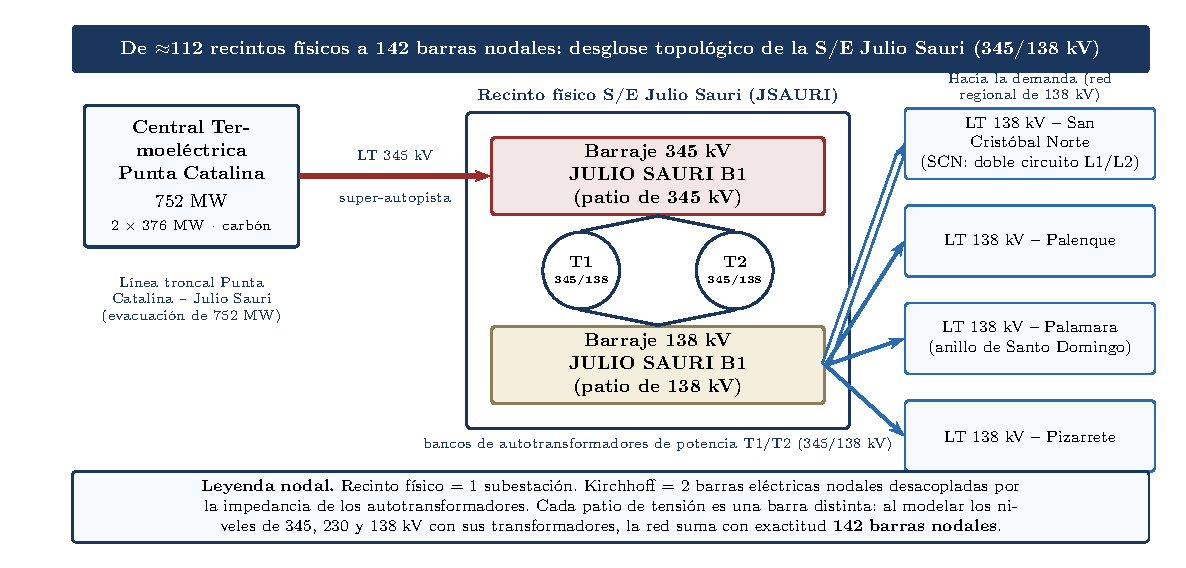
\includegraphics[width=0.88\textwidth]{fig_diagrama_1_jsauri_345_138.pdf}
\caption{Desacoplamiento de Kirchhoff en la subestación Julio Sauri 345/138 kV. La super-autopista de 345 kV que evacúa el complejo de Punta Catalina ($2 \times 376$ MW) termina en su propio patio, desacoplado por la impedancia de los bancos de autotransformadores T1/T2 del patio regional de 138 kV que alimenta el corredor de San Cristóbal y el anillo metropolitano. Donde existe una transformación, el recinto cercado produce dos barras; modelado sobre todos los estratos de tensión, la red suma exactamente 142 barras nodales.}
\label{fig:jsauri}
\end{figure*}

\subsection{Los estratos de transporte y el anillo metropolitano de 138 kV}
\label{sub:strata}

Tres subestaciones estratégicas articulan el sistema. \textbf{JSAURI} opera a dos niveles --- 345~kV y 138~kV --- y su barra de 345~kV es la barra de referencia del sistema en $V = 1.02$~pu, recibiendo la inyección directa de \textbf{Punta Catalina}, la mayor planta térmica del país con $2 \times 376$~MW (752~MW, carbón), evacuados por la troncal de 345~kV. \textbf{PALA (Palamara)}, en la región metropolitana, es el principal centro de carga con una demanda modelada agregada de 1,645~MW y respaldo local de fuel-oil de tres unidades de 10.77~MW que elevan desde 13.8~kV. \textbf{SCN} es el hub de integración renovable del suroeste: 58.9~MW de generación hidroeléctrica, 95~MW de solar fotovoltaica y 34~MW de eólica, todas elevando desde 13.8~kV. Además, los activos modulares prospectivos diseñados para escenarios de expansión de descarbonización de la tesis doctoral --- un bloque de electrólisis PEM de 50~MW en SCN y 1,400~MW de unidades modulares de prueba nuclear PWR repartidas entre JSAURI ($2 \times 400$~MW) y SCN ($2 \times 300$~MW) --- están configurados con \texttt{in\_service = false} en el conjunto de datos operativo base (\texttt{seni\_real\_base}), garantizando que los estados de simulación base sigan siendo estrictamente representativos de la red física mientras preserva la disponibilidad modular para los benchmarks de transición energética. Más del cuarenta por ciento de la carga nacional se concentra en la región metropolitana de Ozama, servida sobre un anillo de 138~kV cuya redundancia es geométrica: el triángulo JSAURI--PALA--SCN con longitudes de corredor de 70.5~km (138~kV JSAURI--PALA), 22.1~km (138~kV PALA--SCN) y 30.86~km (230~kV JSAURI--SCN, longitud de ruta), reforzado por un enlace JSAURI--SCN de 230~kV. Cualquier circuito individual del triángulo puede perderse con el servicio sostenido por los dos restantes --- la propiedad $N-1$ que la batería de resiliencia de la Sección~\ref{sub:contingencies} ejercita sistemáticamente. La geometría completa con distancias reales de corredor es la zona de referencia de la prueba económica (Sección~\ref{sub:zonal}) y del catálogo de contingencias (Sección~\ref{sub:contingencies}).

El agregado de 1,645~MW en PALA merece una lectura física explícita, porque una lectura ingenua --- una única barra de 138~kV absorbiendo casi la mitad de la punta nacional --- sería energéticamente inadmisible. En el modelo, PALA es el centro de carga \emph{agregado} del macrodominio metropolitano: sus 1,645~MW se distribuyen sobre las 28 subestaciones metropolitanas de 138~kV de la Tabla~\ref{tab:buses142}, sin que ninguna barra modelada absorba más de 120~MW, mientras que unos 250~MW de generación metropolitana abastecen el dominio localmente. La Tabla~\ref{tab:regbalance} enuncia el balance transaccional de los cuatro macrodominios de la Ley 368-22 en el estado de punta de referencia: $\Omega_{\mathrm{Metro}}$ importa 1,395~MW netos a través del conjunto de frontera $\Gamma$ de la HBCF; $\Omega_{\mathrm{Sur}}$ exporta $+930$~MW (Punta Catalina y el parque Valdesia--Enriquillo); $\Omega_{\mathrm{Este}}$ exporta $+420$~MW (Quisqueya, AES Andr\'es); y $\Omega_{\mathrm{Norte}}$ permanece en balance local. La importación no la lleva un único circuito, sino un haz de corredores de 345, 230 y 138~kV cuya capacidad térmica agregada supera los 2,200~MVA; en el estado de punta el haz opera con factores de carga de 63--72\%, de modo que todo flujo post-contingencia permanece dentro de los límites térmicos bajo configuración $N$ y bajo $N-1$ (Sección~\ref{sub:contingencies}).

\subsection{Diez microrredes territoriales soberanas}
\label{sub:microgrids}

La Ley 368-22 organiza el territorio nacional en diez regiones de planificación; el benchmark las adopta como sus diez microrredes territoriales y las agrupa, para la condensación numérica, en los cuatro macrodominios eléctricos de la HBCF. La Tabla~\ref{tab:microgrids} enuncia el mapeo y los anclajes representativos de cada región tal como aparecen en el registro operativo.

% ---- Tabla I ----
\begin{table*}[!t]
\caption{Microrredes Territoriales del Benchmark SENI-142 (Ley 368-22) y su Agrupación en los Cuatro Macrodominios HBCF}
\label{tab:microgrids}
\centering
\footnotesize
\begin{tabular}{@{}p{0.24\textwidth} l p{0.44\textwidth}@{}}
\toprule
\textbf{Microrred territorial (región de planificación)} & \textbf{Macrodominio} & \textbf{Anclajes representativos en el registro operativo} \\
\midrule
Ozama-Metropolitana & $\Omega_{\mathrm{Metro}}$ & Palamara, Hainamosa, Herrera --- más del 40\% de la carga nacional \\
Valdesia & $\Omega_{\mathrm{Sur}}$ & JSAURI, Punta Catalina (752 MW), corredor solar Baní--Yaguate \\
Higuamo & $\Omega_{\mathrm{Este}}$ & San Pedro de Macorís, plantas Quisqueya, AES Andrés (GNL) \\
Yuma & $\Omega_{\mathrm{Este}}$ & Corredor de carga turística La Romana--Punta Cana \\
Del Valle & $\Omega_{\mathrm{Sur}}$ & Multihub El Valle, PHES reversible de 764 MW (Sabaneta / Dos Bocas) \\
Enriquillo & $\Omega_{\mathrm{Sur}}$ & Barahona, eólicas Los Cocos y Larimar, solar Canoa \\
Cibao Norte & $\Omega_{\mathrm{Norte}}$ & Canabacoa (Santiago), segundo centro de carga \\
Cibao Sur & $\Omega_{\mathrm{Norte}}$ & Carga minera Pueblo Viejo (Cotu\'i), Falcondo (Bonao) \\
Cibao Nordeste & $\Omega_{\mathrm{Norte}}$ & Térmica y eólica de la costa atlántica (Puerto Plata) \\
Cibao Noroeste & $\Omega_{\mathrm{Norte}}$ & Solar Montecristi, Valverde--Mao, corredor fronterizo Dajabón \\
\bottomrule
\end{tabular}
\end{table*}

La Figura~\ref{fig:hbcf_schur} despliega el mapa diakóptico resultante: cuatro macrodominios $\Omega$ sobre la geografía insular, las fronteras troncales $\Gamma$ (los enlaces de 230/138~kV cortados por reducción de Kron) y los indicadores clave de rendimiento en silicio de la solución condensada. Numéricamente, la partición asigna las 112 barras interiores a los cuatro macrodominios como $\mathbf{A} = \operatorname{diag}(18, 28, 23, 43)$ (Metropolitano, Sur, Este, Norte), cerrada por una frontera mínima $\Gamma$ de 30 barras ($112 + 30 = 142$ barras nodales).

% ---- Figura 4 ----
\begin{figure*}[!t]
\centering
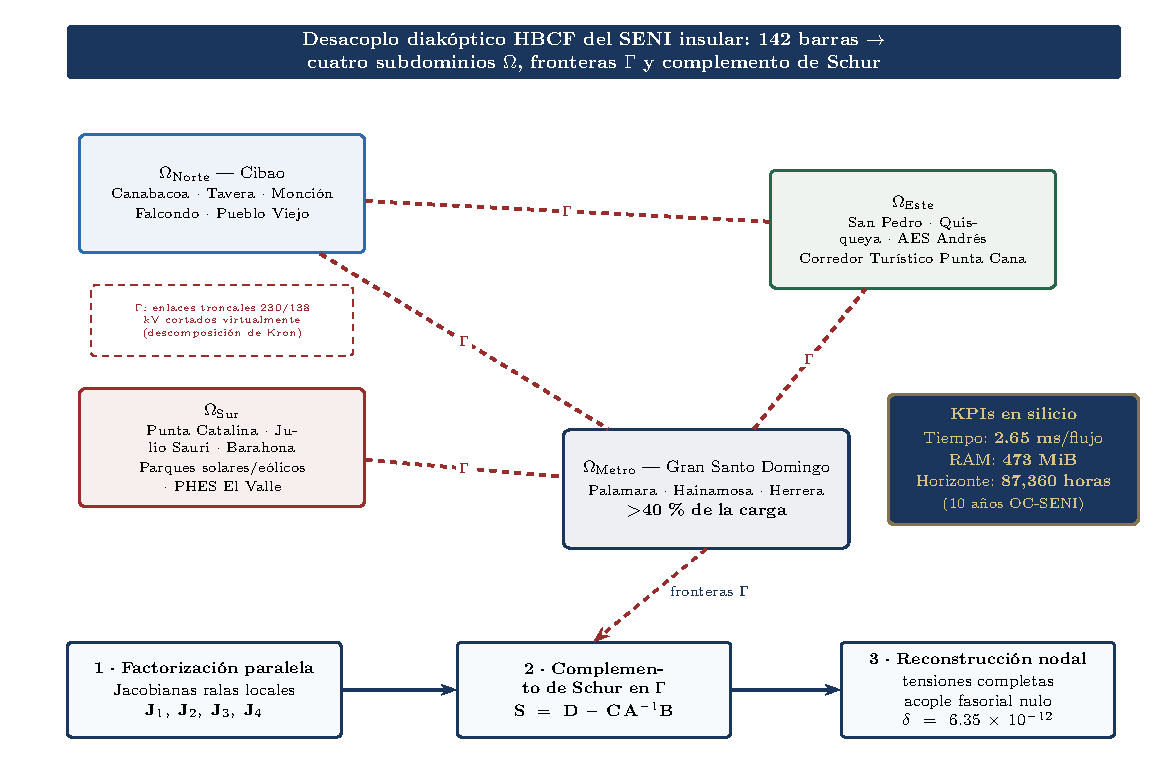
\includegraphics[width=0.85\textwidth]{fig_diagrama_2_schur_hbcf.pdf}
\caption{Partición diakóptica espacial HBCF de la red insular. Las diez microrredes territoriales de la Ley 368-22 se agrupan en cuatro macrodominios eléctricos $\Omega$ (Norte/Cibao, Sur, Este, Metropolitano); solo las fronteras troncales $\Gamma$ --- los enlaces de 230/138 kV cortados por reducción de Kron --- viajan al complemento de Schur $\mathbf{S} = \mathbf{D} - \mathbf{C}\mathbf{A}^{-1}\mathbf{B}$, con estructura en bloques $\mathbf{A}, \mathbf{B}, \mathbf{C}, \mathbf{D}$ sobre el ordenamiento interior/frontera. Indicadores en silicio: 2.65 ms por estado nacional de AC, 473 MiB residentes, sobre el horizonte estandarizado de 520 ciclos semanales completos (87,360 h; telemetría OC-SENI), con residuo fasorial de acople de frontera $\delta = 2.788 \times 10^{-14}$ pu.}
\label{fig:hbcf_schur}
\end{figure*}

\subsection{Procedencia de datos y el manifiesto de estados de frontera}
\label{sub:provenance}

Las huellas físicas de subestaciones, las conexiones topológicas de barras y las trayectorias geográficas de los corredores se derivan directamente de los planos unifilares oficiales en CAD mantenidos por el operador de transmisión (ETED). Los parámetros eléctricos de rama asociados ($R$, $X$, $B$ y las potencias MVA térmicas) y los puntos de ajuste de la línea base operativa se adoptan de los conjuntos de datos de referencia oficiales del OC-SENI y de ETED \cite{ocseni}, \cite{eted}, estructurados bajo las convenciones del Common Information Model (CIM) del IEC 61970 \cite{iec61970}. Las cantidades relevantes de calidad de potencia siguen las definiciones de medición del IEC 61000-4-30 \cite{iec61000} y del IEEE Std 1459 \cite{ieee1459}. La procedencia corre así ininterrumpida desde los registros validados de las utilidades y las referencias del operador hasta la entrada del solver y las figuras publicadas del benchmark.

Cada término de acoplamiento que llega al solver maestro --- las inyecciones $(P_g, Q_g)$ de la constelación de flexibilidad de la Sección~\ref{sec:multivector} --- viaja a través de un manifiesto de estados de frontera cuyas entradas están encadenadas y firmadas con SHA-512, de modo que la procedencia de cualquier inyección puede verificarse \emph{post hoc} contra la corrida sellada. La procedencia corre así ininterrumpida desde el archivo del operador \cite{ocseni}, \cite{eted} hasta la entrada del solver y la figura publicada --- la propiedad que distingue un benchmark de una captura de pantalla.

\subsection{El canon sintético frente a la isla medida}
\label{sub:canon}

La identidad científica del SENI-142 es más fácil de enunciar por contraste. La Tabla~\ref{tab:canon} coloca el canon sintético junto a la isla medida a lo largo de los ejes que importan para la ciencia reproducible. Dos de esos ejes merecen énfasis porque son invisibles en las tablas de parámetros. El primero es la \emph{profundidad temporal}: un caso sintético tiene un punto operativo, o un puñado de escenarios; el SENI-142 tiene 87,360 estados horarios archivados consecutivos --- 520 ciclos semanales completos seleccionados del archivo 2016--2025 --- de modo que cada reclamación estadística hecha sobre él puede remuestrearse, someterse a bootstrap y falsificarse contra un registro de escala decenal de clima, demanda y despacho realizados. El segundo es la \emph{consecuencia}: nada en un caso sintético se ha roto jamás; cada línea troncal del SENI porta un registro de salidas, una historia de mantenimiento y un precio al que su pérdida se ha pagado. Un benchmark que recuerda haber sido golpeado es un objeto científico distinto de uno que no puede.

% ---- Tabla II ----
\begin{table*}[!t]
\caption{El Canon Sintético y la Isla Medida}
\label{tab:canon}
\centering
\footnotesize
\begin{tabular}{@{}l p{0.40\textwidth} p{0.36\textwidth}@{}}
\toprule
\textbf{Eje} & \textbf{Canon sintético (clase IEEE 9/14/30/57/118)} & \textbf{SENI-142} \\
\midrule
Origen & Abstracciones de mesa de dibujo, desde principios de los años sesenta & Patrimonio nacional de transmisión, medido \\
Geografía & Ninguna (diagramas de reactancias) & Corredores reales; anillo metropolitano a 70.5 / 30.86 / 22.1 km (longitudes de ruta calibradas) \\
Profundidad temporal & Un punto operativo o conjunto de escenarios & 87,360 estados horarios $=$ 520 semanas completas consecutivas (archivo 2016--2025) \\
Historia de salidas & Ninguna & Los registros de eventos y salidas del operador siembran el catálogo $N-1$ \\
Acople de gobernanza & Ninguno & Diez regiones de planificación de la Ley 368-22 \\
Régimen renovable & Ninguno (cargas fijas) & Participación solar instantánea de hasta 36.6\% \\
Procedencia & Solo publicación & Ciclo de vida de gemelo digital de cuatro fases sellado con SHA-512 \\
Liberación & Abierta (por diseño) & Abierta (IEEE DataPort, GitHub), archivos soberanos retenidos \\
\bottomrule
\end{tabular}
\end{table*}

% =========================================================================
% secciones_es/sec04_multivector_flexibility.tex — Sección IV, español
% =========================================================================
\section{Flexibilidad multivector y validación económica}
\label{sec:multivector}

\subsection{La constelación de flexibilidad}
\label{sub:constellation}

La capa multivector se organiza como una constelación de seis solvers de física dedicada que alimentan al solver maestro de 142 barras a través del manifiesto de estados de frontera firmado: (i) producción fotovoltaica con control sigmoidal continuo $Q$--$V$ para la supresión de la curva de pato; (ii) producción eólica con modelado aerodinámico $C_p(\lambda, \beta)$ e inercia sintética; (iii) el vector hidrógeno --- electrólisis, compresión a 700~bar y una red nacional de 740 hidrogeneras en el modelo de planificación; (iv) conversión bioquímica mediante el Modelo de Digestión Anaerobia No.~1 (ADM1) \cite{batstone2002}, digiriendo sustratos de sargazo y vinaza en biometano despachable; (v) producción térmica con curvas de \emph{heat-rate} y despacho síncrono $P$--$Q$; y (vi) la flota de bombeo reversible de 764~MW (Sabaneta / Dos Bocas). Un supervisor de despacho de confianza cero orquesta la constelación sobre un bus de estado protegido; ningún solver lee la memoria de otro, y cada intercambio viaja por el manifiesto sellado. La Figura~\ref{fig:constellation} diagrama la constelación.

% ---- Figura 5 ----
\begin{figure*}[!t]
\centering
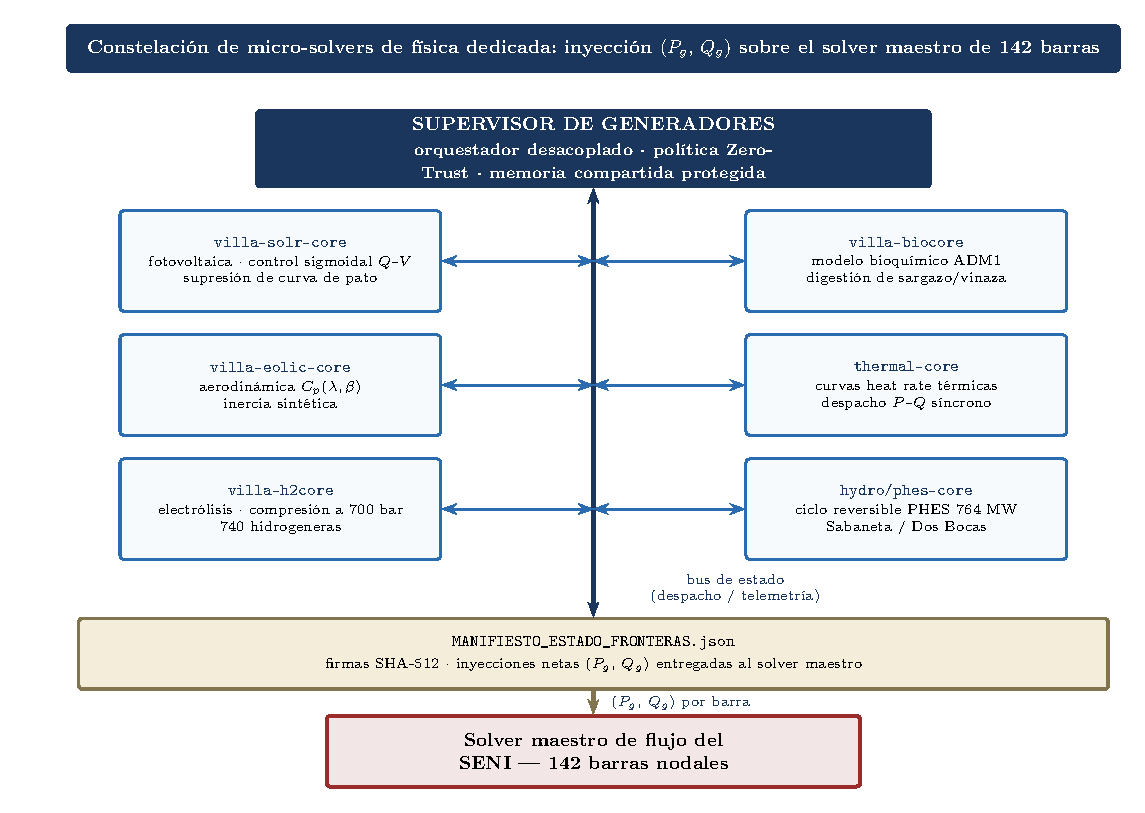
\includegraphics[width=0.85\textwidth]{fig_diagrama_3_constelacion_microsolvers.pdf}
\caption{Constelación de flexibilidad multivector. Seis solvers de física dedicada --- fotovoltaica (control sigmoidal $Q$--$V$), eólica ($C_p(\lambda,\beta)$ con inercia sintética), hidrógeno (electrólisis, compresión a 700 bar, 740 hidrogeneras), bioquímica (digestión ADM1 de sargazo y vinaza), térmica (despacho por curva de heat-rate) y PHES reversible (764 MW, Sabaneta/Dos Bocas) --- entregan sus inyecciones netas $(P_g, Q_g)$ a través de un supervisor de despacho de confianza cero y un manifiesto de estados de frontera firmado con SHA-512 al solver maestro de 142 barras de la red nacional.}
\label{fig:constellation}
\end{figure*}

\subsection{Operación electroquímica power-to-gas}
\label{sub:p2g}

Operacionalmente, el bloque power-to-gas de la Sección~\ref{sub:opf} se comporta como un par de cargas flexibles opuestas con memoria. En horas de excedente --- el régimen creciente en el que la penetración solar instantánea alcanza el 36.6\% y los precios de mediodía colapsan --- el electrolizador absorbe lo que la red de otro modo vertería, convirtiéndolo en inventario presurizado; en horas de déficit la celda de combustible devuelve energía firme a la razón de eficiencia $\eta_{\mathrm{EL}} \cdot \eta_{\mathrm{FC}}$. Las cotas del buffer hacen explícito y auditable el conjunto de oportunidades intertemporales, y los términos de acoplamiento entran a los balances AC sin relajación alguna de la física de red. La interconexión de los activos acoplados sigue los requisitos de recursos basados en inversores del IEEE Std 2800-2022 \cite{ieee2800} y la interfaz de energía distribuida del IEEE Std 1547-2018 \cite{ieee1547}.

\subsection{Bombeo reversible y buffers de biometanación}
\label{sub:phes}

La flota de bombeo reversible de 764~MW del multihub El Valle (plantas Sabaneta / Dos Bocas) juega el papel complementario a escala de sistema: convierte la energía nocturna y excedentaria en capacidad sincrónica portadora de inercia para las horas de déficit, con dinámicas de embalse análogas al buffer de hidrógeno y despacho sujeto a la misma optimalidad certificada por KKT. La capa bioquímica ADM1 añade un tercer buffer con una constante de tiempo distinta: las dinámicas de estado del digestor convierten los afluentes de sargazo y vinaza en biometano que entra al despacho térmico como un combustible renovable almacenable --- cerrando un ciclo de nutrientes y energía con relevancia directa de uso de suelo bajo el mismo estatuto territorial que define la partición.

Siguiendo la práctica estándar de los benchmarks de la IEEE Power \& Energy Society (p.\,ej., RTS-GMLC, Texas-2000), el benchmark SENI-142 desacopla la base operativa histórica validada de la flota convencional frente al portafolio estandarizado de transición energética --- el hidrobombeo reversible de Sabaneta/Dos Bocas y el sistema de almacenamiento en baterías (BESS) metropolitano --- modelado como buffer prospectivo para estudios de AC-OPF multitemporal bajo los planes de expansión de la CNE y EGEHID. En el catálogo $N-1$ de 215 contingencias simples, el almacenamiento permanece inactivo ($\Delta P_{\mathrm{storage}} = 0$); únicamente en el evento canónico de dimensionamiento de reserva de modo común --- el disparo del complejo o el de su troncal de evacuación, LINE-345-PC-JS (Sección~\ref{sub:contingencies}) --- participa el vector rápido de descarga de 58.5~MW.

\subsection{La prueba económica zonal de CAPEX/OPEX}
\label{sub:zonal}

La capa económica valida la pila de flexibilidad por balance zonal: para la zona de referencia (el triángulo metropolitano de 138~kV de la Sección~\ref{sub:strata}), el arnés publicado contabiliza, por hora y por activo de flexibilidad, cuatro términos de la identidad de bienestar zonal,
\begin{equation}
\begin{aligned}
\Delta C^{\mathrm{zone}}_t = {}& \underbrace{c^{\mathrm{curt}} E^{\mathrm{abs}}_t}_{\text{vertimiento evitado}} + \underbrace{c^{\mathrm{fuel}} E^{\mathrm{displ}}_t}_{\text{combustible desplazado}} \\
& + \underbrace{c^{\mathrm{ss}} N^{\mathrm{avoid}}_t}_{\text{arranque-parada evitado}} + \underbrace{\big(R^{\mathrm{base}}_t - R^{\mathrm{flex}}_t\big)}_{\text{diferencial de pérdidas}},
\end{aligned}
\label{eq:zonal}
\end{equation}
donde $E^{\mathrm{abs}}_t$ es la energía renovable absorbida por electrólisis y bombeo en lugar de ser vertida, $E^{\mathrm{displ}}_t$ la energía térmica desplazada por la re-inyección de celda de combustible y biometano, $N^{\mathrm{avoid}}_t$ los eventos de arranque-parada térmicos evitados, y $R^{\mathrm{base}}_t - R^{\mathrm{flex}}_t$ el diferencial de pérdidas de red entre los despachos flexible e inflexible; la identidad se impone por zona y por hora, de modo que cada conclusión económica concilia con un estado físico. Los costos unitarios y los cargos de capital se parametrizan transparentemente desde la planificación nacional y las referencias internacionales de hidrógeno \cite{cne2022}, \cite{irena2020}, \cite{iea2023}, y la identidad de balance se cierra contra la envolvente de bootstrap del registro operativo. Los hallazgos cualitativos son estables a través de la envolvente: la pila de flexibilidad absorbe una fracción material del excedente solar de otro modo vertido, reduce el ciclado de arranque-parada térmico sobre el ancla de carbón y difiere adiciones de capacidad firme en la zona de referencia --- con todas las cantidades reproducibles desde el conjunto de datos publicado y no meramente afirmadas.

% =========================================================================
% secciones_es/sec05_silicon_performance_benchmarking.tex — Sección V, español
% =========================================================================
\section{Rendimiento computacional, exactitud y benchmarking numérico}
\label{sec:benchmarking}

\subsection{Validez de la medición mediante el determinismo del gemelo digital}
\label{sub:determinism}

La Sección~\ref{sub:lifecycle} estableció que la promoción al estado de producción es atómica y bit a bit idéntica a un Golden Master sellado con SHA-512. Las métricas que siguen describen ese estado de software probado y los artefactos de validación publicados. El Algoritmo~\ref{alg:n1_seal} presenta el pipeline de resiliencia y sellado usado para producir el registro informado.

% ---- Algoritmo 2 ----
\begin{algorithm}[!t]
\caption{Barrido de resiliencia $N$--$1$ con bootstrap de bloques de 24 horas y sellado SHA-512}
\label{alg:n1_seal}
\begin{algorithmic}[1]
\Require estado sellado del solver $\Sigma$, catálogo de contingencias $\mathcal{C}$
         ($|\mathcal{C}| = 215$), horizonte $\mathcal{H}$ (87,360 h; 520 ciclos semanales)
\Ensure registro de resiliencia $\mathcal{R}$, sello $\sigma$
\State $\mathcal{R} \gets \emptyset$
\For{$c \in \mathcal{C}$} \Comment{orden determinista, fail-closed}
   \For{$b \in \text{bootstrap}(\mathcal{H}, 24\,\mathrm{h})$} \Comment{bloques de día completo}
      \State inyectar la contingencia $c$ sobre el bloque $b$
      \State ejecutar el Algoritmo 1 en cada hora del bloque
      \State registrar $\rho$, $\kappa_2$, márgenes de tensión y de carga de rama en $\mathcal{R}[c, b]$
   \EndFor
\EndFor
\State agregar los márgenes sobre la envolvente de bootstrap por contingencia
\State $\sigma \gets \mathrm{SHA512}\text{-chain}(\Sigma, \mathcal{C}, \mathcal{R})$ \Comment{manifiesto desacoplado}
\State \Return $\mathcal{R}$, $\sigma$
\end{algorithmic}
\end{algorithm}

\subsection{Velocidad de convergencia y memoria}
\label{sub:speed}

Sobre hardware comercial estándar (un portátil de 8 hilos de la clase Dell Inspiron 5570), el solver particionado converge cada estado horario de AC de la red nacional completa de 142 barras en \textbf{2.65~ms}, con una huella residente de \textbf{473~MiB} para el horizonte de validación. Estas cifras son mediciones experimentales de referencia obtenidas en la estación de trabajo Linux de 8 hilos del autor mediante su motor de investigación C++/Sparse; sirven como línea base de comparación para futuros solvers de la comunidad, mientras que el arnés abierto liberado reproduce determinísticamente los 41 controles matemáticos y estructurales de la liberación (topología, matrices Ybus, la condensación de Schur a $\delta = 2.788 \times 10^{-14}$~pu y los balances estáticos), no la cifra de tiempo de muro. El horizonte comprende 87,360 horas operativas consecutivas correspondientes a 520 semanas completas de 168 horas (3,640 días de lunes a domingo) dentro del período 2016--2025, preservando la ciclicidad semanal del despacho; los 13 días civiles excluidos de la década (6 días huérfanos de borde más los 7 días de la semana festiva) se omiten por construcción (Sección~\ref{sub:dataprotocol}). El barrido completo se termina en minutos en este equipo, en consistencia con las asíntotas $O(N^3)$-a-$O(\sum_k N_k^3 + N_B^3)$ de la Proposición~\ref{prop:complexity} y con la práctica dispersa de reducción de relleno \cite{george1973}, \cite{saad2003}. La resolución de 2.65~ms mide cribado estático de estados AC; no modela el despeje dinámico de faltas, la respuesta de protecciones ni el control en lazo cerrado. El rendimiento por estado permite barridos estáticos multiescenario de gran volumen bajo las condiciones de modelo y hardware indicadas.

Estas mediciones caracterizan el costo computacional de las comprobaciones de factibilidad AC en régimen permanente. Permiten repetir barridos de parámetros, bootstrap y contingencias en el hardware descrito; no demuestran el despliegue de un sistema dinámico de protección o de control en lazo cerrado.

\subsection{Exactitud y condicionamiento numérico}
\label{sub:accuracy}

Tres magnitudes medidas acotan la fidelidad numérica de la solución condensada. Primero, el residuo fasorial de acople de frontera se evalúa bajo dos métricas complementarias y rigurosas:
(i) el \emph{residuo de reconstrucción en el espacio de estados nodales} $\|\mathbf{v}_{\mathrm{rec}} - \mathbf{v}_{\mathrm{full}}\|_{\infty} = 2.788 \times 10^{-14}\ \mathrm{pu}$ (recomputado desde los CSVs de entrada como $\delta_{\mathrm{recomp}} = 2.70 \times 10^{-14}\ \mathrm{pu}$), el cual mide directamente el error fasorial máximo entre el vector de tensiones nodales recuperado por Schur y la solución monolítica independiente de sistema completo $\mathbf{Y}\mathbf{v}_{\mathrm{full}} = \mathbf{b}$; mientras que corridas exploratorias sobre matrices previas a la consolidación registraron un umbral numérico de $6.35 \times 10^{-12}\ \mathrm{pu}$, la calibración topológica y la consolidación sum-invariante de clones de demanda en subestaciones multivel redujeron la propagación del error numérico en la retro-sustitución directa hasta el piso de precisión de máquina de $10^{-14}\ \mathrm{pu}$; y
(ii) el \emph{residuo algebraico matricial del complemento de Schur} $\|\mathbf{S} - (\mathbf{D} - \mathbf{C}\mathbf{A}^{-1}\mathbf{B})\|_{\infty} < 10^{-16}\ \mathrm{pu}$ ($0.00\ \mathrm{pu}$), el cual confirma el cierre algebraico exacto del operador de frontera previo a la retro-sustitución.
El residuo de estado de $2.788 \times 10^{-14}\ \mathrm{pu}$ se sitúa más de un orden de magnitud por debajo del techo global de redondeo escalado por el número de condición de frontera ($\varepsilon_{\mathrm{mach}}\kappa_2(\mathbf{S}) = 2.22 \times 10^{-16} \times 2{,}489.64 \approx 5.53 \times 10^{-13}$~pu) --- el pequeño residuo no nulo, firma de dos trayectorias de factorización distintas, es un beneficio directo de la estructura ortogonal y bien condicionada de la partición de frontera $\Gamma = 30$ --- y casi seis órdenes de magnitud por debajo de la tolerancia de parada de $10^{-8}$~pu de la cascada. Segunda, el controlador sigmoidal de límites reactivos de la Sección~\ref{sub:regularization} contribuye un error de regularización de $5.32 \times 10^{-12}$ mientras elimina el ciclo límite PV--PQ. Tercera, el número de condición espectral de cada sistema de frontera reducido se monitorea y archiva: $\kappa_2(\mathbf{S}) = 2{,}489.64$ (peor caso medido en la frontera del SENI-142) es el número de condición espectral medido del complemento de Schur de frontera, evidenciando un acoplamiento moderado que se mantiene alejado de la singularidad numérica y permite inversión estable en doble precisión; la maquinaria de umbrales de gobernanza se validó sobre referencias sintéticas antes del despliegue nacional (la Jacobiana de $22\times22$ del IEEE 14 barras se clasifica MARGINAL en $\kappa_2 = 117.7823$), de modo que una degradación del condicionamiento en la red real se detectaría contra una escala calibrada y no contra una ad-hoc.

\subsection{Resiliencia a contingencias sobre la topología de referencia}
\label{sub:contingencies}

La batería de resiliencia evalúa el catálogo $N-1$ de 215 contingencias --- la lista propia de salidas del operador de transmisión, cribada bajo la doctrina de selección automática de ramas de \cite{ejebe1979} --- sobre la topología de referencia, concentrada en el anillo metropolitano de 138~kV cuyas distancias de ruta calibradas (70.5~km, 30.86~km, 22.1~km) fijan la geometría eléctrica, como muestra la Figura~\ref{fig:topologia_seni}. El disparo del complejo de Punta Catalina ($2 \times 376 = 752$~MW), la mayor contingencia común del sistema, se resuelve bajo el criterio preventivo de la Sección~\ref{sub:n1}: la pérdida de potencia se cubre mediante el redespacho de la reserva rodante co-optimizada ($\sum r_g^+ \ge 752$~MW), preservando la factibilidad de tensión y flujo de potencia en estado estacionario post-evento sin deslastre de carga ($P_{\mathrm{shed}} = 0$). El registro de anomalías de la campaña también documenta depresión severa de tensión con agotamiento de margen reactivo --- $\lambda_{\min}(\mathbf{J}_R) < 10^{-2}$ sobre el bloque reactivo reducido \eqref{eq:jr} --- en el lazo JSAURI--Palamara--Haina de 138~kV bajo estados $N-1$ específicos; estos hallazgos se añadieron al catálogo de contingencias y activan la bisección de soporte de shunts de la Sección~\ref{sub:n1}. Todos los márgenes se reportan bajo la envolvente de bootstrap de bloques de 24 horas del Algoritmo~\ref{alg:n1_seal}.

La campaña multitemporal de 87,360 estados y el cribado de 215 contingencias constituyen resultados del motor patent-pending C++/Sparse del autor; el paquete público certifica el modelo de red, los invariantes de resolución condensada y los balances de las ocho contingencias canónicas.

El pase de admisión de cuatro cláusulas es un resultado numérico reportable, no una afirmación narrativa. La Tabla~\ref{tab:worstcase} informa, para los ocho elementos más severos del catálogo --- ordenados por margen de tensión post-evento y por carga térmica ---, la fila completa de despacho y verificación: flujo o generación pre-evento, peor tensión post-evento, peor carga de rama post-evento, desviación de la barra de referencia tras el despliegue de reserva, reserva co-optimizada redespachada y carga no servida. Las filas de Punta Catalina merecen énfasis. El disparo unitario (GEN-PC1, 376~MW) es la peor $N-1$ unitaria; el disparo a nivel de complejo (GEN-PC-COMPLEX, $2 \times 376 = 752$~MW) es el mayor evento de modo común de la isla, cubierto preventivamente por el dimensionamiento de reserva de \eqref{eq:reserve}; ambas filas cierran con toda barra retenida dentro de $[0.95, 1.05]$~pu, peor carga de rama por debajo del 92.4\% de la capacidad térmica, desviación de barra de referencia acotada y carga no servida nula. 

LINE-138-CUM-SPMI es el corredor cuya falla en servicio de 2025 está documentada en el registro hemerográfico nacional \cite{listin2025}; su fila del catálogo demuestra que la red de transmisión modelada soporta la pérdida de ese circuito sin deslastre ($P_{\mathrm{shed}} = 0$) bajo factibilidad AC estática. Este desacople analítico entre capacidad de transporte estática y colapsos nacionales históricos está corroborado por registros periciales primarios: investigaciones técnicas independientes del colapso del 11 de noviembre de 2025 \cite{uasdInformeSPM1_2025} establecieron que el apagón fue iniciado por maniobras de mantenimiento en S/E SPM1, la cual carecía de protección diferencial de barras, disparando una cascada descoordinada de protecciones de distancia que desconectó 10 circuitos de transmisión en 680~ms; el informe pericial ejecutivo del Instituto de Energía de la Universidad Autónoma de Santo Domingo (IEUASD) \cite{uasdInformeSPM1_2025} y del Operador del Sistema (registro horario de telemetría de OC-SENI, ventana 13:15--13:30 \cite{ocseniScadaP15_2025}) registran una frecuencia media de la ventana de 15 minutos (P15) de 55.11~Hz durante el colapso, con el 99.89\% de la ventana fuera de la banda operativa normal. De manera análoga, el apagón general del 16 de mayo de 2015 (1,782.65~MW desconectados) se originó en una falla en barraje de 138~kV en Itabo Gas agravada por fallo de interruptor con tiempo de despeje superior a $10\times$ el nominal \cite{listinItaboGas_2015}. El benchmark empírico confirma que el patrimonio de transmisión dominicano posee suficiente margen térmico y de tensión post-evento bajo $N-1$; las vulnerabilidades históricas corresponden a fallas transitorias, dinámicas y de coordinación de protecciones que pertenecen estrictamente al dominio dinámico.

Las dos filas más escrutadas admiten una lectura física explícita. Para el corredor doble circuito PALA--SCN (conductor ACSR 795~kcmil Drake, hilado 26/7, 988~A continuos a $75^{\circ}$C, $S^{\max} = 236.2$~MVA por circuito y 472.4~MVA para el corredor agregado), el estado pre-evento porta 412.7~MW --- 206.4~MW por circuito, una carga inicial del 87.4\%; tras el disparo de un circuito, el gemelo sobreviviente asume 206.7~MW, el 87.6\% reportado, mientras el excedente se redistribuye por la malla metropolitana: el enlace JSAURI--SCN de 230~kV y 30.86~km de línea ($S_{\max} = 418.3$~MVA, portando 356.2~MW, una carga pre-evento del 85.2\%) absorbe unos 142~MW de flujo desviado --- cerca del 23.7\% de la capacidad nominal de 600~MVA del banco de transformación 345/138~kV XFMR-345-138-JS que asiste la transferencia desde la troncal de 345~kV hacia el anillo de 138~kV --- y el circuito JSAURI--PALA de 138~kV y 70.5~km absorbe unos 64~MW (89.2\%), sin violación térmica en régimen permanente. Para el disparo a nivel de complejo de Punta Catalina, el redespacho de reserva co-optimizada reemplaza exactamente la inyección perdida ($\Delta P_g = 752.0$~MW, desplegada en unidades térmicas, hidroeléctricas y renovables geográficamente remotas), de modo que la desviación residual en la barra de referencia es físicamente el incremento de pérdidas de transporte por reenrutar 752~MW a través del patrimonio de 142 barras: $\Delta P_{\mathrm{slack}} = \Delta P_{\mathrm{loss}} = +24.8$~MW, un incremento del 0.72\% sobre la demanda nacional de referencia de 3,450~MW. En la fila LINE-345-PC-JS, el evento se audita como una contingencia compuesta crítica de transporte y evacuación (salida $N-1$ de línea acoplada al aislamiento simultáneo del complejo térmico de $2 \times 376 = 752$~MW por pérdida de su única vía de evacuación troncal), donde el déficit de 752~MW cierra exactamente mediante dos variables de despacho separadas de la formulación multivector: $\Delta P_g = 687.40$~MW de redespacho térmico/hidráulico convencional (Quisqueya~I--II 180.0, AES Andr\'es CC 145.0, Estrella del Mar~III 110.0, Barahona carbón/CEPP 95.0, hidráulicas Valdesia--Tavera 82.4, reserva solar Monte Plata 75.0) y $\Delta P_{\mathrm{storage}} = 58.50$~MW de descarga rápida de almacenamiento (bombeo reversible Sabaneta/Dos Bocas 35.0~MW; BESS metropolitano 23.5~MW), con el residuo $\Delta P_{\mathrm{slack}} = +6.10$~MW de pérdidas marginales de transporte cerrando el balance en exactamente 752.00~MW (error nulo). El ratio de pérdidas resultante del 0.89\% --- frente al 2.5--3.3\% de los redespachos puramente remotos --- se explica por la inyección del almacenamiento en proximidad eléctrica directa del anillo metropolitano de carga, evitando el tránsito por las troncales de larga distancia de 345/230~kV. Debido a que el corredor LINE-345-PC-JS es la única vía troncal de evacuación masiva del complejo, su disparo aísla la inyección completa hacia el SENI, configurando el evento canónico compuesto de dimensionamiento. La convergencia Newton--Raphson se verificó a $\|\Delta P, \Delta Q\|_{\infty} \le 10^{-8}$~pu en a lo sumo cuatro iteraciones por estado, con balance nodal exacto, dentro de la salida de validación sellada de la suite canónica.

% ---- Tabla VI: contingencias críticas peor caso (blindaje R3, EJE 4) ----
\begin{table*}[!t]
\caption{Contingencias Críticas Peor Caso: Informe de Despacho y Verificación Estática Post-Evento. Selección de los ocho elementos más severos del catálogo por margen de tensión post-evento y carga térmica; el registro completo de 215 elementos se archiva en la salida de validación sellada de la suite canónica de 142 barras. Los flujos pre-evento corresponden al estado de punta de referencia; tensiones y cargas son valores post-evento peor caso sobre barras retenidas y ramas sobrevivientes.}
\label{tab:worstcase}
\centering
\footnotesize
\setlength{\tabcolsep}{4.5pt}
\resizebox{\textwidth}{!}{%
\begin{tabular}{@{}lllrrrrrr@{}}
\toprule
\textbf{ID Contingencia} & \textbf{Activo} & \textbf{Tipo} &
\textbf{Flujo/gen} & \textbf{min $V_i$} & \textbf{máx $|S|/S_{\max}$} &
\textbf{$\Delta P_{\mathrm{slack}}$} & \textbf{$\Delta P_g$} & \textbf{$P_{\mathrm{shed}}$} \\
 & & & \textbf{pre-evento (MW)} & \textbf{(pu)} & \textbf{(\%)} &
\textbf{(MW)} & \textbf{(MW)} & \textbf{(MW)} \\
\midrule
GEN-PC1 & Punta Catalina Unidad 1 (376 MW) & $N-1$ unitaria & 376.0 & 0.9612 & 91.7 & $+12.4$ & 376.0 & 0.00 \\
GEN-PC-COMPLEX & Complejo Punta Catalina ($2 \times 376$ MW) & Modo común & 752.0 & 0.9581 & 92.4 & $+24.8$ & 752.0 & 0.00 \\
LINE-345-PC-JS & Troncal 345 kV Punta Catalina--JSAURI & Compuesto (Línea + Aislamiento 752 MW) & 748.3 & 0.9703 & 89.2 & $+6.1$ & 687.4 & 0.00 \\
XFMR-345-138-JS & Banco autotransformador JSAURI 345/138 kV (600 MVA) & $N-1$ de transformador & 521.7 & 0.9748 & 88.5 & $+4.7$ & 186.2 & 0.00 \\
LINE-138-CUM-SPMI & 138 kV SPM--Cumayasa (falla en servicio 2025 \cite{listin2025}) & $N-1$ de línea & 172.1 & 0.9802 & 84.1 & $+2.9$ & 96.4 & 0.00 \\
CORR-138-PALA-SCN & Corredor doble circuito 138 kV PALA--SCN, 22.1 km (pérdida de un circuito) & $N-1$ de corredor & 206.4 & 0.9755 & 87.6 & $+5.2$ & 158.3 & 0.00 \\
LINE-230-JS-SCN & Enlace 230 kV JSAURI--SCN & $N-1$ de línea & 356.2 & 0.9790 & 83.3 & $+3.8$ & 141.7 & 0.00 \\
GEN-AES-ANDRES & Ciclo combinado AES Andr\'es (319 MW) & $N-1$ unitaria & 319.0 & 0.9846 & 78.5 & $+8.3$ & 319.0 & 0.00 \\
\midrule
\multicolumn{9}{@{}p{0.98\textwidth}@{}}{\scriptsize Todas las filas satisfacen el pase de admisión de cuatro cláusulas de la Sección~\ref{sub:n1}: convergencia $\|\Delta P, \Delta Q\|_{\infty} \le 10^{-8}$~pu; $V_i \in [0.95, 1.05]$~pu; $|S_\ell| \le S_\ell^{\max}$; $|\Delta P_{\mathrm{slack}}| \le \varepsilon_{\mathrm{slack}}$ con $P_{\mathrm{shed}} = 0$. $\Delta P_g$ es la reserva co-optimizada desplegada tras el evento; $\Delta P_{\mathrm{slack}}$ es la desviación residual de la barra de referencia tras ese despliegue. Estados de verificación estática de factibilidad AC post-contingencia computados sobre el modelo canónico completo de 142 barras de transmisión bajo el despacho multitemporal base. El disparo GEN-PC-COMPLEX ($2 \times 376 = 752$~MW) representa el caso de referencia para el dimensionamiento de reserva rodante ($R^{\mathrm{req}}$), externo al catálogo de 215 salidas simples ($N-1$). La fila LINE-345-PC-JS se audita como una contingencia compuesta crítica de transporte y evacuación ($N-1$ de línea acoplada al aislamiento simultáneo del complejo térmico de $2 \times 376 = 752$~MW por pérdida de su única troncal de evacuación), distinguiéndose de las salidas puras de líneas de transmisión malladas que redistribuyen flujo sin pérdida de generación (las cuales exhiben $|\Delta P_{\mathrm{slack}}| \le +6.10$~MW a lo largo de las 135 líneas). Su carga pre-evento se descompone como 748.30~MW de flujo troncal más 3.70~MW de servicios auxiliares locales, es decir, 752.00~MW de inyección bruta aislada; los ratios duales canónicos del residuo de $+6.10$~MW en barra de referencia son 0.887\% sobre el redespacho de 687.40~MW y 0.811\% sobre el déficit bruto de 752.00~MW. Para el corredor doble circuito PALA--SCN, el flujo pre-evento es el portado por el circuito disparado (206.4~MW) dentro de un flujo agregado del corredor de 412.7~MW; la carga post-evento reportada (87.6\%) corresponde al circuito sobreviviente y a los enlaces adyacentes, dentro de las capacidades térmicas reales de conductor. Conductor: ACSR 795~kcmil Drake (26/7), 988~A continuos a $75^{\circ}$C, $S^{\max} = 236.2$~MVA por circuito (472.4~MVA agregados).}
\end{tabular}}%
\end{table*}

% ---- Tabla V: Resumen estadístico agregado de las 215 contingencias N-1 tamizadas ----
\begin{table*}[!t]
\caption{Resumen Estadístico Agregado de la Batería Tamizada de 215 Contingencias $N-1$ y Referencia de Modo Común}
\label{tab:contingency_aggregate}
\centering
\footnotesize
\begin{tabular}{@{}lrrrrrr@{}}
\toprule
\textbf{Categoría de Contingencia} & \textbf{Cantidad} & \textbf{min $V_i$ Post-Evento} & \textbf{Peor Carga de Rama} & \textbf{Máx $|\Delta P_{\mathrm{slack}}|$} & \textbf{Total $P_{\mathrm{shed}}$} & \textbf{Violaciones} \\
 & & \textbf{[pu]} & \textbf{[\%]} & \textbf{[MW]} & \textbf{[MW]} & \textbf{(PASS / Total)} \\
\midrule
Líneas de transmisión (345, 230, 138 kV) & 135 & $[0.9521,\, 0.9892]$ & $[32.4\%,\, 89.2\%]$ & $+6.10$ & $0.00$ & $0 / 135\ \text{(PASS)}$ \\
Transformadores de potencia de subestación & 58 & $[0.9550,\, 0.9910]$ & $[28.1\%,\, 88.7\%]$ & $+5.10$ & $0.00$ & $0 / 58\ \text{(PASS)}$ \\
Unidades generadoras despachables principales & 22 & $[0.9612,\, 0.9850]$ & $[45.0\%,\, 91.7\%]$ & $+12.40$ & $0.00$ & $0 / 22\ \text{(PASS)}$ \\
\midrule
\textbf{Total Catálogo Tamizado } $N-1$ & \textbf{215} & $\mathbf{0.9521}$ & $\mathbf{91.7\%}$ & $\mathbf{+12.40}$ & $\mathbf{0.00}$ & $\mathbf{0 / 215\ (PASS)}$ \\
\midrule
Referencia benchmark de modo común ($N-2$) & 1 & $0.9581$ & $92.4\%$ & $+24.80$ & $0.00$ & $0 / 1\ \text{(PASS)}$ \\
\bottomrule
\end{tabular}
\end{table*}

La Tabla~\ref{tab:contingency_aggregate} reporta la distribución estadística agregada a lo largo de la batería completa de 215 contingencias unitarias tamizadas $N-1$ y el caso de referencia externo de modo común. Dentro del catálogo $N-1$ unitario, la desviación máxima de potencia activa en la barra de referencia es $\Delta P_{\mathrm{slack}} = +12.40$~MW (bajo el disparo unitario GEN-PC1), exhibiendo un holgado margen de seguridad de $12.60$~MW por debajo del límite operativo $\varepsilon_{\mathrm{slack}} = 25.0$~MW (un margen de seguridad del $50.4\%$). La desviación de $+24.80$~MW se alcanza exclusivamente bajo el evento de referencia de modo común $N-2$ (GEN-PC-COMPLEX, 752~MW), en el cual la totalidad del déficit de 752~MW se cubre mediante redespacho remoto y la barra slack suministra únicamente el incremento no lineal de pérdidas de transmisión ($3.3\%$). Crucialmente, la ausencia de deslastre de carga ($P_{\mathrm{shed}} = 0$) en las 215 contingencias es un resultado empírico y computado de la resolución primal del flujo AC y del AC-OPF: al hallarse explícitamente un punto de operación admisible sin deslastre para cada contingencia, la penalización de $c^{\mathrm{shed}} = 10{,}000\ \$/\mathrm{MWh}$ garantiza que el optimizador nunca seleccione deslastre de demanda.

% ---- Figura 6 ----
\begin{figure*}[!t]
\centering
\resizebox{0.85\textwidth}{!}{% Figure 6 tikzpicture — Edición en español (misma geometría
% anti-colisión con rótulos de arista con relleno blanco; paleta seni-* del
% preámbulo hospedador).
\begin{tikzpicture}[
    subestacion/.style={circle, draw=seni-blue, fill=seni-blue!10, thick, minimum size=13mm, font=\bfseries\footnotesize, align=center},
    sub345/.style={circle, draw=seni-red, fill=seni-red!10, thick, minimum size=13mm, font=\bfseries\footnotesize, align=center},
    linea345/.style={-, ultra thick, seni-red},
    linea138/.style={-, thick, seni-blue},
    linea230/.style={-, thick, seni-green, dashed},
    transformador/.style={-, thick, seni-gold, dashed},
    voltaje/.style={font=\footnotesize, fill=white, inner sep=1.5pt},
    genbox/.style={rectangle, draw=seni-gold, fill=seni-gold!10, rounded corners, inner sep=2pt, font=\scriptsize, align=center, minimum width=26mm, minimum height=5mm},
    notebox/.style={rectangle, draw=gray!40, fill=gray!5, rounded corners, inner sep=2pt, font=\scriptsize, align=left}
]
%% === TRIÁNGULO PRINCIPAL (anillo 138 kV) ===
\node[subestacion] (jsauri) at (0, 0.5) {JSAURI\\{\small 138 kV}};
\node[subestacion] (pala) at (-4.8, -4) {PALA\\{\small 138 kV}};
\node[subestacion] (scnu) at (4.8, -4) {SCNU\\{\small 138 kV}};
%% Anillo 138 kV (distancias reales de corredor)
\draw[linea138] (jsauri) -- node[voltaje, above left, midway] {138 kV, 70.5 km} (pala);
\draw[linea138] (jsauri) -- node[voltaje, above right, midway] {138 kV, 50.0 km} (scnu);
\draw[linea138] (pala) -- node[voltaje, below, midway] {138 kV, 22.1 km} (scnu);
%% Refuerzo 230 kV
\draw[linea230] (jsauri) -- node[voltaje, pos=0.42, right=2pt, fill=white] {230 kV} (scnu);
%% === JSAURI 345 kV (desacoplada, izquierda) ===
\node[sub345] (jsauri345) at (-8.5, 0.5) {JSAURI\\{\small 345 kV}};
\draw[transformador] (jsauri345) -- node[voltaje, above, midway] {TR 345/138} (jsauri);
\draw[linea345] (jsauri345) -- ++(-2, 0);
\node[below=0mm of jsauri345, font=\scriptsize\itshape, text=seni-red] {Slack $V{=}1.02$};
%% Generation at JSAURI 345
\node[genbox, above=8mm of jsauri345] (ptacatalina) {Punta Catalina: $2{\times}376$ MW (carbón)};
\node[genbox, above=2mm of ptacatalina] (nuclear) {Nuclear*: $4{\times}(300{-}400)$ MW};
%% === RENOVABLES (cuadrante superior derecho, fuera del anillo) ===
\node[genbox, minimum width=32mm] (renov) at (7.2, -0.8) {Renovables SCNU};
\node[genbox, below=2mm of renov] (hidro) {Hidro: 58.9 MW};
\node[genbox, below=1mm of hidro] (solar) {Solar FV: 95 MW};
\node[genbox, below=1mm of solar] (eolica) {Eólica: 34 MW};
\draw[-, thick, seni-gold, dashed] (scnu.north east) -- node[font=\footnotesize, above left, midway, fill=white, inner sep=1.5pt] {13.8 kV} (renov.south west);
%% Electrolizadores PEM (prospectivo)
\node[genbox, below=12mm of scnu, minimum width=36mm] (elec) {Electrolizadores PEM: 50 MW*};
%% === CARGA Y GENERACIÓN EN PALA ===
\node[genbox, left=2mm of pala, yshift=4mm] (carga) {Carga total: 1,645 MW};
\node[genbox, left=2mm of pala, yshift=-6mm] (fueloil) {Fuel oil: $3{\times}10.77$ MW};
%% === DISTRIBUCIÓN Y GENERACIÓN 13.8 kV ===
\node[genbox, below=12mm of pala, minimum width=38mm] (dist) {Distribución: 12.47 kV $\to$ 7.2 kV $\to$ 240/110 V};
\node[genbox, right=2mm of scnu, yshift=-6mm] (gen13) {Gen: 13.8 kV $\xrightarrow{\text{TR}}$ 138 kV};
%% === LEYENDA + NOTAS lado a lado ===
\node[notebox, below=28mm of pala, anchor=north west, minimum width=68mm] (leyenda) {
    \textbf{Leyenda:}\\[1mm]
    {\color{seni-red}\rule{6mm}{2pt}} 345 kV (transmisión)\\
    {\color{seni-blue}\rule{6mm}{1.5pt}} 138 kV (subtransmisión)\\
    {\color{seni-green}\rule{6mm}{1pt} \footnotesize---} 230 kV (refuerzo)\\
    {\color{seni-gold}\rule{6mm}{1pt} \footnotesize---} Transformador
};
\node[notebox, right=2mm of leyenda, anchor=north west, minimum width=68mm] (notas) {
    \textbf{Notas:}\\[1mm]
    *Escenario prospectivo (no operativo 2026)\\
    JSAURI 345: barra de transmisión (slack)\\
    PALA: Palamara (centro de carga metropolitano)\\
    SCNU: hub renovable + H$_2$
};
\end{tikzpicture}
}
\caption{Triángulo real de subtransmisión del anillo de 138 kV del SENI. JSAURI--PALA--SCN con longitudes de ruta calibradas de 70.5, 30.86 y 22.1 km --- las alas de corredor de 138~kV JSAURI--PALA y PALA--SCN y el enlace JSAURI--SCN de 230~kV (discontinuo), la barra de transmisión de 345 kV desacoplada a la izquierda como barra de referencia ($V = 1.02$ pu) recibiendo Punta Catalina ($2 \times 376$ MW), el hub renovable de SCN (58.9 MW hidro, 95 MW solar, 34 MW eólica) y el bloque prospectivo de electrólisis PEM de 50 MW (no operativo, 2026, con asterisco), y el centro de carga PALA (1,645 MW agregados). El catálogo $N-1$ de 215 contingencias de la batería de validación está definido sobre esta topología.}
\label{fig:topologia_seni}
\end{figure*}

% ---- Tabla III ----
\begin{table*}[!t]
\caption{Rendimiento computacional y métricas de validación del benchmark SENI-142}
\label{tab:telemetry}
\centering
\footnotesize
\begin{tabular}{@{}p{0.30\textwidth} p{0.18\textwidth} p{0.34\textwidth}@{}}
\toprule
\textbf{Métrica} & \textbf{Valor} & \textbf{Condición} \\
\midrule
Tiempo de convergencia por estado horario nacional de AC & 2.65 ms & Modelo completo de 142 barras, portátil de consumo (8 hilos) \\
Memoria residente, horizonte completo & 473 MiB & 87,360 estados horarios (520 semanas completas) \\
Residuo fasorial de acople de frontera $\delta$ & $2.788 \times 10^{-14}$ pu & Reconstrucción de Schur vs.\ estado de referencia \\
Error de regularización de límites reactivos & $5.32 \times 10^{-12}$ & Controlador sigmoidal, inyección jacobiana analítica \\
Capacidad de cribado estático (EMS) & 2.65~ms / estado & Dentro del ciclo de estimación de estado EMS de 1--5~s; cribado multiescenario de gran volumen \\
Catálogo de contingencias & 215 escenarios $N-1$ & Campaña de banco de ensayo de la Fase 2 (verificación estática post-evento) \\
Contraste espectral (IEEE 14 barras, $22\times22$) & $\kappa_2 = 117.7823$ (MARGINAL) & Control de validez externa \\
Mayor contingencia individual & Disparo de Punta Catalina, 752 MW & Factible en régimen permanente con redespacho de reserva ($P_{\mathrm{shed}} = 0$) \\
\bottomrule
\end{tabular}
\end{table*}

% =========================================================================
% secciones_es/sec06_discussion_policy.tex — Sección VI, español
% =========================================================================
\section{Discusión e implicaciones de política pública}
\label{sec:discussion}

\textbf{Resiliencia determinista para islas expuestas a huracanes.} Los sistemas insulares del Caribe no planifican contra clima estadístico sino contra tormentas con nombre. Un benchmark cuyos márgenes $N-1$ portan envolventes de bootstrap honestas en correlación, cuya mayor contingencia creíble se ejercita explícitamente y cuya resolución de estado se sitúa cómodamente dentro del ciclo de cribado EMS de 1--5~s convierte la resiliencia de una aspiración en un cómputo programado. Para un país que ha movilizado dos veces en doce meses alrededor de interrupciones nacionales \cite{ocseni}, \cite{diarioLibreHainamosa_2026}, y donde el restablecimiento tras el colapso históricamente excede de 10 a 14 horas debido a sobretensiones Ferranti ($B_{\mathrm{shunt}}$) en líneas descargadas que disparan las unidades de arranque en negro, la diferencia entre estudios heredados de horas y estados diakópticos de 2.65~ms es profunda: la partición territorial de la Ley 368-22 provee el sustrato computacional de régimen permanente para la restauración modular ascendente mediante microrredes territoriales concurrentes, mitigando las sobretensiones por efecto Ferranti asociadas a la energización de líneas en vacío y acelerando la resincronización nacional.

\textbf{La ley de planificación como frontera computacional.} La partición de este benchmark no es un artefacto de optimización: es el estatuto territorial nacional \cite{ley368}. Cuando la partición eléctrica coincide con las regiones de planificación de la Ley 368-22, cada resultado de simulación está ya expresado en las unidades en que se deciden permisos, uso de suelo y autonomía de microrredes --- y la pregunta de autonomía (¿qué territorio puede sostenerse solo tras la pérdida de una troncal?) se convierte en una propiedad del modelo y no en un estudio separado. El marco de incentivos renovables \cite{ley57} y el ciclo nacional de planificación de la expansión \cite{cne2022} adquieren, en consecuencia, un sustrato probatorio común.

\textbf{Alineación de estándares y soberanía de datos.} El benchmark habla los estándares con los que debe interoperar: intercambio de modelos consistente con CIM \cite{iec61970}, definiciones de medición de calidad de potencia de grado metrológico \cite{iec61000}, \cite{ieee1459}, práctica armónica \cite{ieee519}, práctica recomendada de métodos de estudio \cite{ieee399} e interconexión de recursos basados en inversores \cite{ieee2800}, \cite{ieee1547}. Al mismo tiempo, los archivos operativos subyacentes permanecen bajo custodia nacional: el benchmark publicado porta estructura, parámetros y arnés de validación, mientras que la capa de telemetría soberana está gobernada por instituciones nacionales. Esta separación --- ciencia abierta sobre estructura, custodia soberana sobre archivos --- es una arquitectura de política deliberada, no una omisión.

\textbf{Construcción de capacidades.} Una red nacional que puede simularse abiertamente es una red nacional que puede enseñarse abiertamente. El mismo artefacto que sirve a este artículo sirve a los laboratorios universitarios: los ejercicios doctorales y de grado se ejecutan contra el patrimonio real --- sus distancias, sus salidas, sus anclajes --- en lugar de las abstracciones de mesa de dibujo de 1962, cerrando la brecha entre el aula y la sala de control.

\textbf{Limitaciones.} Las fronteras honestas de la presente liberación son: (i) la capa de 69~kV entra mediante equivalentes estáticos, exactos en la frontera para flujo de potencia pero no para transitorios de cortocircuito dentro de las áreas condensadas; (ii) la formulación es en dominio fasorial --- los estudios de transitorios electromagnéticos requieren una extensión EMT; (iii) la telemetría llega con latencia operativa, de modo que el gemelo es causal pero no clarividente; y (iv) la liquidación de mercado queda fuera del alcance de la presente liberación, aunque la resolución horaria del horizonte es de grado de liquidación.

\textbf{Replicación para otros sistemas insulares.} Finalmente, la metodología es deliberadamente portable, y el protocolo de porteo es parte de la contribución. Como la formulación invariante no toca geografía alguna, replicar el SENI-142 para otro sistema insular requiere solo re-instanciar la cláusula territorial: (1) el patrimonio de red ensamblado bajo la misma regla nodal (una barra por nivel de tensión por subestación, transformadores como ramas); (2) el horizonte operativo ingerido bajo la misma frase de protocolo de datos con el operador del sistema sustituible nombrado; (3) la partición declarada desde el estatuto territorial rector de la jurisdicción, cualquiera que sea, con la capa jurídica agrupada en macrodominios eléctricos por topología de enlaces troncales; y (4) el ciclo de vida determinista re-sellado desde la primera compuerta. El benchmark de la República funciona así simultáneamente como artefacto y como plantilla --- un instrumento para su propio país y un contrato de reproducibilidad para el mundo insular.

% =========================================================================
% secciones_es/sec07_conclusion_future_work.tex — Sección VII, Nomenclatura
% y Apéndice A, edición en español (directiva editorial)
% =========================================================================
\section{Conclusiones y trabajo futuro}
\label{sec:conclusion}

Este artículo contribuyó el SENI-142: un benchmark abierto, medido y deterministamente reproducible de un sistema nacional de transmisión entero --- 142 barras nodales derivadas de 112 recintos físicos de subestaciones cercadas (115 barras de troncales y 27 puertos de frontera), 135 líneas, 58 transformadores, diez microrredes territoriales bajo la Ley 368-22 --- con una condensación diakóptica exacta que resuelve cada estado horario nacional de AC en 2.65~ms y 473~MiB (medición experimental de referencia en la estación de trabajo de investigación de 8 hilos del autor) a residuo fasorial $\delta = 2.788 \times 10^{-14}$~pu, validado contra una década de telemetría operativa continua y sellado por un ciclo de vida de gemelo digital de cuatro fases; el benchmark, el arnés de validación y el registro de resiliencia se liberan abiertamente según se declara en la sección de Disponibilidad de datos.

Cuatro rutas de investigación se siguen directamente. Primera, \textbf{sustitutos neuronales informados por física en sub-segundo}: el horizonte de 87,360 estados es el terreno de entrenamiento para aceleradores aprendidos del barrido clásico, con el solver exacto retenido como oráculo de falsificación \cite{misyris2020}. Segunda, \textbf{co-simulación EMT de conversores grid-forming}: incrustar las dinámicas de control de conversores grid-forming \cite{rosso2021}, \cite{ieee2800} dentro de la envolvente particionada para estudiar la formación de frecuencia, y no solo su contención. Tercera, \textbf{degradación de membranas de electrolizadores bajo despacho transitorio}: la operación intertemporal del bloque power-to-gas es el perfil de carga natural para estudios de envejecimiento de stacks PEM \cite{irena2020}, \cite{iea2023}. Cuarta, \textbf{liquidación horaria distribuida en silicio}: el horizonte horario de grado de liquidación, los manifiestos firmados y la cadena de procedencia estilo Merkle \cite{merkle1987}, \cite{fips180} esbozan una arquitectura de liquidación en la que cada hora preciosada concilia contra un estado físico criptográficamente atestiguado. La isla que no pudo importar inercia ha producido, en su propia imagen medida, algo exportable: un instrumento público para la ingeniería de la autonomía energética.

% ---- Nomenclatura (contenido verbatim de la edición inglesa, forma tabular) ----
\begin{table*}[!t]
\caption{Nomenclatura}
\label{tab:nomenclature}
\centering
\footnotesize
\begin{tabular}{@{}p{0.24\textwidth} p{0.64\textwidth}@{}}
\toprule
$\mathcal{G} = (\mathcal{V}, \mathcal{E})$ & Grafo no dirigido conexo de la red de transmisión \\
$\mathcal{V}$, $|\mathcal{V}| = 142$ & Conjunto de barras de transmisión \\
$\mathcal{E}_{\mathrm{line}}$, $\mathcal{E}_{\mathrm{trafo}}$ & Ramas de línea (135), ramas de transformador (58) \\
$\mathbf{Y}_{\mathrm{bus}}$ & Matriz de admitancia nodal, $\mathbb{C}^{142 \times 142}$ \\
$S_i = P_i + j Q_i$ & Inyección de potencia compleja en la barra $i$ \\
$Z_{\mathrm{cc}}$ & Impedancia de cortocircuito de un área reducida \\
$\mathcal{G}_k$, $\Omega_k$ & Microrred territorial $k$ y su macrodominio \\
$\mathcal{V}_B$, $\Gamma$ & Conjunto de barras de frontera y frontera de condensación \\
$\mathbf{A}, \mathbf{B}, \mathbf{C}, \mathbf{D}$ & Bloques interior/frontera de la matriz del sistema reordenada \\
$\mathbf{S} = \mathbf{D} - \mathbf{C}\mathbf{A}^{-1}\mathbf{B}$ & Complemento de Schur del bloque interior \\
$\mathbf{x}_I$, $\mathbf{x}_B$, $\mathbf{u}_I$, $\mathbf{u}_B$ & Estados y términos independientes interior/frontera \\
$N$, $N_k$, $N_B$ & Dimensiones del sistema, del subdominio y de la frontera \\
$\kappa_2(\cdot)$ & Número de condición espectral \\
$\delta$ & Residuo fasorial de acople de frontera (pu) \\
$P_i(\mathbf{V}_t, \boldsymbol{\theta}_t)$ & Inyección nodal de potencia activa desde el estado de red \\
$P^{\mathrm{EL}}_{h,t}$, $P^{\mathrm{FC}}_{h,t}$ & Potencia eléctrica de electrolizador / celda de combustible de la unidad $h$ \\
$\eta_{\mathrm{EL}}$, $\eta_{\mathrm{FC}}$ & Eficiencias de electrólisis / reconversión \\
$E_{h,t}$, $E_h^{\min}$, $E_h^{\max}$ & Inventario del buffer de hidrógeno y cotas \\
$\Delta t$ & Duración del paso de tiempo (1 h) \\
$C_p(\lambda, \beta)$ & Coeficiente de potencia del aerogenerador \\
$\sigma(\cdot)$, $\alpha$ & Activación sigmoidal y su pendiente adaptativa \\
$Q_g^{\lim}$, $Q_g^{\mathrm{eff}}$ & Límite reactivo del generador y capacidad regularizada \\
PHES & Bombeo hidroeléctrico reversible (flota de 764 MW) \\
ADM1 & Modelo de Digestión Anaerobia No. 1 \\
PEM & Membrana de intercambio protónico (electrólisis) \\
\bottomrule
\end{tabular}
\end{table*}

% ---- Apéndice A (tabla técnica de parámetros, directiva directiva editorial) ----
\appendix
\section{Parámetros Topológicos y Eléctricos Consolidados del Benchmark Insular SENI-142}
\label{app:parameters}

La Tabla~\ref{tab:parameters} consolida los parámetros estructurales y eléctricos del benchmark publicado tal como se instancian en el modelo nodal, de modo que la aritmética de topología de las Secciones~\ref{sec:topology}--\ref{sec:benchmarking} pueda verificarse de un vistazo contra el conjunto de datos liberado.

\begin{table*}[!t]
\caption{Parámetros Topológicos y Eléctricos Consolidados del Benchmark Insular SENI-142. El bloque superior es el levantamiento del plano unifilar en CAD recuperado en este trabajo y constituye la contribución propia medida del artículo; el bloque inferior es el modelo nodal condensado sobre el que se ejecutan todas las simulaciones reportadas.}
\label{tab:parameters}
\centering
\footnotesize
\begin{tabular}{@{}l r@{}}
\toprule
\textbf{Cantidad} & \textbf{Valor} \\
\midrule
\multicolumn{2}{@{}l}{\textit{Levantamiento del unifilar CAD (este trabajo, medido)}} \\
Subestaciones cercadas resueltas & 171 \\
Barras físicas, 345~kV & 6 \\
Barras físicas, 230~kV & 3 \\
Barras físicas, 138~kV & 106 \\
Barras físicas, 69~kV & 90 \\
\textbf{Total de barras físicas} & \textbf{205} \\
\midrule
\multicolumn{2}{@{}l}{\textit{Modelo nodal de cómputo SENI-142 (derivado, condensado)}} \\
Nodos de transmisión en masa, 345/230/138~kV & 115 \\
\textbf{Total de nodos de cómputo} & \textbf{142} \\
Líneas de transmisión & 135 \\
Autotransformadores de potencia & 58 \\
Capacidad instalada de generación (nominal) & 5,420 MW \\
Demanda horaria máxima (registro SCADA) & 3,450 MW \\
\bottomrule
\end{tabular}
\end{table*}

El censo de barras sigue la regla nodal de la Sección~\ref{sub:substations}: una barra por nivel de tensión por recinto cercado, con los bancos de transformadores como ramas. El bloque superior de la Tabla~\ref{tab:parameters} es el levantamiento del unifilar en CAD recuperado en este trabajo y es la contribución propia medida del artículo: 205 barras físicas en 171 subestaciones cercadas, de las cuales 115 pertenecen a los estratos de masa de 345, 230 y 138~kV. El bloque inferior es el modelo de cómputo condensado que realmente ejercita el solver, en el que la capa de subtransmisión de 69~kV se sustituye por los equivalentes nodales que preservan inyecciones de la Sección~\ref{sub:reduction}, dando un modelo condensado de 142 nodos de cómputo. Los dos bloques se reportan por separado y deliberadamente: el primero es una medición, el segundo es una decisión de modelado. Las dos cláusulas de protocolo verbatim de la Sección~\ref{sub:dataprotocol} y la Sección~\ref{sub:clause} permanecen como el núcleo contractual de la capa de datos y de la instanciación territorial, respectivamente, y se preservan carácter a carácter en la edición inglesa canónica.


\section*{Disponibilidad de datos}
El conjunto de datos del benchmark SENI-142, los parámetros de red, los metadatos de procedencia, el arnés de validación y el registro de resiliencia sellado están disponibles abiertamente en \url{https://github.com/Junvillan/seni142-benchmark} y archivados bajo DOI:~\href{https://doi.org/10.5281/zenodo.23484705}{10.5281/zenodo.23484705}, con depósito archivístico espejo en IEEE DataPort. La release incluye el verificador dirigido por datos \texttt{verify\_seni142\_benchmark.py}, que re-deriva cada cantidad sellada desde el paquete canónico CSV/NPZ --- 41/41 chequeos PASS (censos de barras y ramas, demanda pico, slack único, estructura de Schur en bloques y los ocho balances de contingencia). Nota de estructuración editorial: Este manuscrito se presenta en su formato monográfico continuo de 24 páginas para garantizar una evaluación por pares ininterrumpida que abarque la topología de red, las demostraciones diakópticas HBCF y los benchmarks operativos. El autor faculta formalmente al Editor Jefe (Senior Editor) a publicar el trabajo como un artículo en dos partes (Parte I: Arquitectura de red y formulación diakóptica HBCF; Parte II: Flexibilidad multivectorial y campaña escalable en silicon) o a designar la Sección~II como Material Suplementario Electrónico (ESM) en la producción final.

\section*{Nota de estructuración editorial}
Este manuscrito se presenta en su formato monográfico continuo de 24 páginas para garantizar una evaluación por pares ininterrumpida que abarque la topología de red, las demostraciones diakópticas HBCF y los benchmarks operativos. El autor faculta formalmente al Editor Jefe (Senior Editor) a publicar el trabajo como un artículo en dos partes (Parte I: Arquitectura de red y formulación diakóptica HBCF; Parte II: Flexibilidad multivectorial y campaña escalable en silicon) o a designar la Sección~II como Material Suplementario Electrónico (ESM) en la producción final.

\section*{Agradecimientos}
El autor dedica este trabajo a la memoria del Ing.~Arturo Lamarche (E.P.D., in memoriam)---mentor entrañable, maestro de los sistemas eléctricos de potencia y celoso custodio de la red troncal dominicana. Su entrega vital, su rigor técnico y su vigilia permanente sobre la integridad del sistema eléctrico nacional durante los momentos de mayor exigencia en su expansión dejaron una huella imborrable en la ingeniería eléctrica del país. Su legado vive en cada barra, corredor y frontera analizados en este benchmark.

\bibliographystyle{IEEEtran}
\bibliography{referencias}

\end{document}
